%%%%%%%%%%%%%%%%%%%%%%%%%
% Dokumentinformationen %
%%%%%%%%%%%%%%%%%%%%%%%%%
\newcommand{\titleinfo}{Robotik - Formelsammlung}
\newcommand{\authorname}{Luca Mazzoleni}

%Buch
%Industrieroboter - Methoden der Steuerung und Regelung
%3., neu bearbeiete Auflage
%Wolfgang Weber
%Isbn: 978-3-446-43355-7

%BuG-Fix
%Package pdf Error: Driver file ................ not found
%If you have a luatex driver fail uncomment these lines
%\RequirePackage{luatex85}
%\def\pgfsysdriver{pgfsys-pdftex.def}

% Genereller Header
\documentclass[11pt,twoside,a4paper,fleqn]{article}
% Dateiencoding
\usepackage[utf8]{inputenc}
\usepackage[T1]{fontenc}	%ä,ü...
% Seitenränder
\usepackage[left=1cm,right=1cm,top=0.5cm,bottom=0.2cm,includeheadfoot]{geometry}
\setlength{\headsep}{5pt} 
% Sprachpaket
\usepackage[english, ngerman]{babel} % Silbentrennung und Rechtschreibung Englisch und Deutsch

%%%%%%%%%%%%%%%%%%%%%%%
%% Wichtige Packages %%
%%%%%%%%%%%%%%%%%%%%%%%

\usepackage{amsmath}                % Allgemeine Matheumgebungen									
\usepackage{amssymb}                % Fonts: msam,msbm, eufm & Mathesymbole, Mengen (lädt automatisch amsfonts)									
\usepackage{array}                  % \newcolumntype, \firsthline, ,\lasthline, m{width}, b{width}									
\usepackage{caption}                % Bildunterschriften									
\usepackage{enumitem}               % basic environments: enumerate, itemize, description									
\usepackage{fancybox}               % \fbox: \shad­ow­box, \dou­ble­box, \oval­box, \Oval­box									
\usepackage{fancyhdr}               % Seiten schöner gestalten, insbesondere Kopf- und Fußzeile									
\usepackage{floatflt}               % Textumflossene Abbildungen \begin{floatingfigure}[r]{Breite} : r rechts, l links, p links auf geraden Seiten und rechts auf ungeraden Seiten									
\usepackage{graphicx}               % \includegraphics[keyvals]{imagefile}, [draft]graphicx zeigt nur Namen und Rahmen an, [final] hebt diese option auf => Bild wird angezeigt    									
\usepackage{hyperref}               % Erstellt Verweise innerhalb und nach außerhalb eines PDF Dokumentes.								
\usepackage{lastpage}               % Bspw. : Page 1 of 3 => \thepage\ of \pageref{LastPage}									
\usepackage{listings}               % Erlaubt es Programmcode in der gewünschten Sprache zu hinterlegen (C++, Matlab,..). Definition der Sprache mit \lstset{language=name}..									
\usepackage{longtable}              % Longtable erlaubt es Tabellen zu erstellen die bei der nächsten Seite weiterlaufen. (Bricht automatisch um)									
\usepackage{mathabx}                % Mathesymbole									
\usepackage{mathrsfs}               % \mathscr (Benötigt für Fourierreihen-Symbol)									
%\usepackage{mathtools}              % Extension package to amsmath									
\usepackage{multicol}               % multicols-Umgebung \begin{multicols}{3} erzeugt Abschnitt mit 3 Spalten									
\usepackage{multirow}               % Tabelle: ermöglicht es Felder mehrerer Zeilen in einem zusammenzufassen									
\usepackage{pdflscape}              % adds PDF support to the environment 'landscape'									
\usepackage{pxfonts}                % Symbole, griechisches Alphabet, Integrale...									
\usepackage{rotating}               % sideways, turn{degree}, rotate{degree}, sidewaysfigure, sidewaystable Umgebung									
\usepackage{subcaption}             % Bildunterschriften für Subfigures									
\usepackage{tabularx}               % tabularx-Umgebung: Hat feste Gesamtbreite, \begin{tabularx}{\textwidth}{c c c c c} X: Spalte mit variabler Breite, l, c, r, p{breite}, m{breite}									
\usepackage{textcomp}               % text symbols: baht, bullet, copyright, musical-note, onequarter, section, yen									
\usepackage{tikz}                   % Tikz Umgebung zur Grafikerzeugung									
\usepackage{titlesec}               % Überschriften zu Textabstände
\usepackage{trfsigns}               % Transformationszeichen \laplace, \Laplace..									
\usepackage{trsym}                  % Weitere Laplace Zeichen erlaubt auch vertikale Transformationszeichen									
\usepackage{verbatim}               % verbatim, verbatim*, comment Umgebung									
\usepackage{wrapfig}                % Textumflossene Bilder und Tabellen, \begin{wrapfigure}[Zeilen]{Position}[Ueberhang]{Breite}									
\usepackage{xcolor}                 % \pagecolor{color}, \textcolor{color}{text}, \colorbox{color}{text}, \fcolorbox{border-color}{fill-color}{text}									
\usepackage{titlesec}
% Zum Bilder einfach in Tabellen einfügen (valign=t)
\usepackage[export]{adjustbox}

%%%%%%%%%%%%%%%%%%%%
% Generelle Makros %
%%%%%%%%%%%%%%%%%%%%
\newcommand{\skript}[1]{$_{\textcolor{red}{\mbox{\small{Skript S.#1}}}}$}
\newcommand{\verweis}[2]{\small{(siehe auch \ref{#1}, #2 (S. \pageref{#1}))}}
\newcommand{\verweiskurz}[1]{(\small{siehe \ref{#1}\normalsize)}}
\newcommand{\subsubadd}[1]{\textcolor{black}{\mbox{#1}}}
\newcommand{\formelbuch}[1]{$_{\textcolor{red}{\mbox{\small{S#1}}}}$}

\newcommand{\robos}[1]{$_{\textcolor{red}{\mbox{\small{Ind.Rob S. #1}}}}$}
\newcommand{\robo}[2]{$_{\textcolor{red}{\mbox{\small{Ind.Rob S. #1 K. #2}}}}$}
\newcommand{\stoecker}[1]{$_{\textcolor{grey}{\mbox{\small{Stöcker #1}}}}$}
\newcommand{\sachs}[1]{$_{\textcolor{blue}{\mbox{\small{Sachs S. #1}}}}$}
\newcommand{\hartl}[1]{$_{\textcolor{green}{\mbox{\small{Hartl S. #1}}}}$}

\newcommand{\schaum}[1]{\tiny Schaum S. #1}

\newcommand{\skriptsection}[2]{\section{#1 {\tiny Skript S. #2}}}
\newcommand{\skriptsubsection}[2]{\subsection{#1 {\tiny Skript S. #2}}}
\newcommand{\skriptsubsubsection}[2]{\subsubsection{#1 {\tiny Skript S. #2}}}

\newcommand{\matlab}[1]{\footnotesize{(Matlab: \texttt{#1})}\normalsize{}}

% Syntax: \bmu{Pfad zum Bild}{Bildgrösse}{Beschriftung des Bildes}
\newcommand{\bl}[2]{
	\begin{figure}[h]
		\flushleft  % linksbuendig
		\includegraphics[width=#1]{#2} \\
	\end{figure}
}
\newcommand{\br}[2]{
	\begin{figure}[h]
		\flushright  % rechtsbuendig
		\includegraphics[width=#1]{#2} \\
	\end{figure}
}

\newcommand{\bild}[2]{
	\begin{figure}[h]
		\centering  % zentriert
		\includegraphics[width=#1]{#2} \\
	\end{figure}
}

\newcommand\tabbild[2][]{%
	\raisebox{0pt}[\dimexpr\totalheight+\dp\strutbox\relax][\dp\strutbox]{%
		\includegraphics[#1]{#2}%
	}%
}

\newcolumntype{P}[1]{>{\raggedright\arraybackslash}p{#1}} %Tabelle linksausgerichtet
\newcolumntype{L}[1]{>{\raggedleft\arraybackslash}p{#1}} %Tabelle rechtsausgerichtet
\newcolumntype{C}[1]{>{\centering\arraybackslash}p{#1}}


\setitemize{noitemsep,topsep=0pt,parsep=0pt,partopsep=0pt} %kompakte itemize
\setenumerate{noitemsep,topsep=0pt,parsep=0pt,partopsep=0pt} %kompakte enumerate

%%%%%%%%%%
% Farben %
%%%%%%%%%%
\definecolor{black}{rgb}{0,0,0}
\definecolor{red}{rgb}{1,0,0}
\definecolor{white}{rgb}{1,1,1}
\definecolor{grey}{rgb}{0.8,0.8,0.8}
\definecolor{green}{rgb}{0,.8,0.05}
\definecolor{brown}{rgb}{0.603,0,0}
\definecolor{mymauve}{rgb}{0.58,0,0.82}


%%%%%%%%%%%%%%%%%%%%%%%%%%%%
% Mathematische Operatoren %
%%%%%%%%%%%%%%%%%%%%%%%%%%%%
\DeclareMathOperator{\sinc}{sinc}
\DeclareMathOperator{\sgn}{sgn}
\DeclareMathOperator{\Real}{Re}
\DeclareMathOperator{\Imag}{Im}
%\DeclareMathOperator{\e}{e}
\DeclareMathOperator{\cov}{cov}
\DeclareMathOperator{\PolyGrad}{PolyGrad}

%Grösse Integral anpassen
\def\Int{\mbox{\Large$\displaystyle\int$\normalsize}}
\def\OInt{\mbox{\Large$\displaystyle\oint$\normalsize}}

%Makro für 'd' von Integral- und Differentialgleichungen 
\newcommand*{\diff}{\mathop{}\!\mathrm{d}}

%%%%%%%%%%%%%%%%%%%%%%%%%%%
% Fouriertransformationen %
%%%%%%%%%%%%%%%%%%%%%%%%%%%

% Fouriertransformationen
\unitlength1cm
\newcommand{\FT}
{
	\begin{picture}(1,0.5)
	\put(0.2,0.1){\circle{0.14}}\put(0.27,0.1){\line(1,0){0.5}}\put(0.77,0.1){\circle*{0.14}}
	\end{picture}
}


\newcommand{\IFT}
{
	\begin{picture}(1,0.5)
	\put(0.2,0.1){\circle*{0.14}}\put(0.27,0.1){\line(1,0){0.45}}\put(0.77,0.1){\circle{0.14}}
	\end{picture}
}


%%%%%%%%%%%%%%%%%%%%%%%%%%%%
% Allgemeine Einstellungen %
%%%%%%%%%%%%%%%%%%%%%%%%%%%%

%Pdf Info
\hypersetup{pdfauthor={\authorname},pdftitle={\titleinfo},colorlinks=false}
\author{\authorname}
\title{\titleinfo}

% Abstände Text zu Übertiteln / Einzug
\titlespacing{\section}{12pt}{1em}{0.5em}
\titlespacing{\subsection}{12pt}{1em}{0.5em}
\titlespacing{\subsubsection}{12pt}{1em}{0.5em}

%%%%%%%%%%%%%%%%%%%%%%%
% Kopf- und Fusszeile %
%%%%%%%%%%%%%%%%%%%%%%%
\pagestyle{fancy}
\fancyhf{}
%Linien oben und unten
\renewcommand{\headrulewidth}{0.5pt} 
\renewcommand{\footrulewidth}{0.5pt}

%Kopfzeile links bzw innen
\fancyhead[L]{\titleinfo{ }}
%Kopfzeile mitte
%\fancyhead[C]{}
%Kopfzeile rechts bzw. aussen
\fancyhead[R]{Seite \thepage { }von \pageref{LastPage}}

%Fusszeile links bzw. innen
\fancyfoot[L]{\footnotesize{\authorname}}
%Fusszeile mitte
%\fancyfoot[C]{\footnotesize{\authoremail}}
%Fusszeile rechts bzw. ausen
\fancyfoot[R]{\footnotesize{\today}}
% Einrücken verhindern versuchen
\setlength{\parindent}{0pt}

%%%%%%%%%%%%%%%%%%%%%%%%%%%%%%%%%%%%%%%
%% Makros & anderer Low-Level bastel %%
%%%%%%%%%%%%%%%%%%%%%%%%%%%%%%%%%%%%%%%
% Zeilenhöhe Tabellen:
\newcommand{\arraystretchOriginal}{1.5}
\renewcommand{\arraystretch}{\arraystretchOriginal}

\makeatletter
%% Makros für den Arraystretch (bei uns meist in Tabellen genutzt, welche Formeln enthalten)
% Default Value
\def\@ArrayStretchDefault{1} % Entspricht der Voreinstellung von Latex

% Setzt einen neuen Wert für den arraystretch
\newcommand{\setArrayStretch}[1]{\renewcommand{\arraystretch}{#1}}

% Setzt den arraystretch zurück auf den default wert
\newcommand{\resetArrayStretch}{\renewcommand{\arraystretch}{\@ArrayStretchDefault}}

% Makro zum setzten des Default arraystretch. Kann nur in der Präambel verwendet werden.
\newcommand{\setDefaultArrayStretch}[1]{%
    \AtBeginDocument{%
        \def\@ArrayStretchDefault{#1}
        \renewcommand{\arraystretch}{#1}
    }
}
\makeatother

%% Achtung Symbol \danger
\newcommand*{\TakeFourierOrnament}[1]{{%
        \fontencoding{U}\fontfamily{futs}\selectfont\char#1}}
\newcommand*{\danger}{\TakeFourierOrnament{66}}



\begin{document} 
\maketitle
\clearpage
\setcounter{tocdepth}{3}
\footnotesize
\tableofcontents
\thispagestyle{empty}
\normalsize
\clearpage
%%%%%%%%%%%%%%%%%%%%%%%%%%%%%%%%%%%%%%%%%%%%%%%%%%%%%%%%%%%%%%%%%%%%%%%%%%%%%%%%
\section{Roboterkomponenten}
\textbf{Die Asimov’schen Gesetze}\newline
\begin{enumerate}
    \item Ein Roboter darf kein menschliches Wesen verletzen oder durch Untätigkeit zulassen, dass einem menschlichen Wesen Schaden zugefügt wird.
    \item Ein Roboter muss den ihm von einem Menschen gegebenen Befehlen gehorchen – es sei denn, ein solcher Befehl würde mit Regel eins kollidieren.
    \item Ein Roboter muss seine Existenz beschützen, solange dieser Schutz nicht mit Regel eins oder zwei kollidiert.
\end{enumerate}
\begin{minipage}{0.5\linewidth}
\subsection{Genauigkeit}
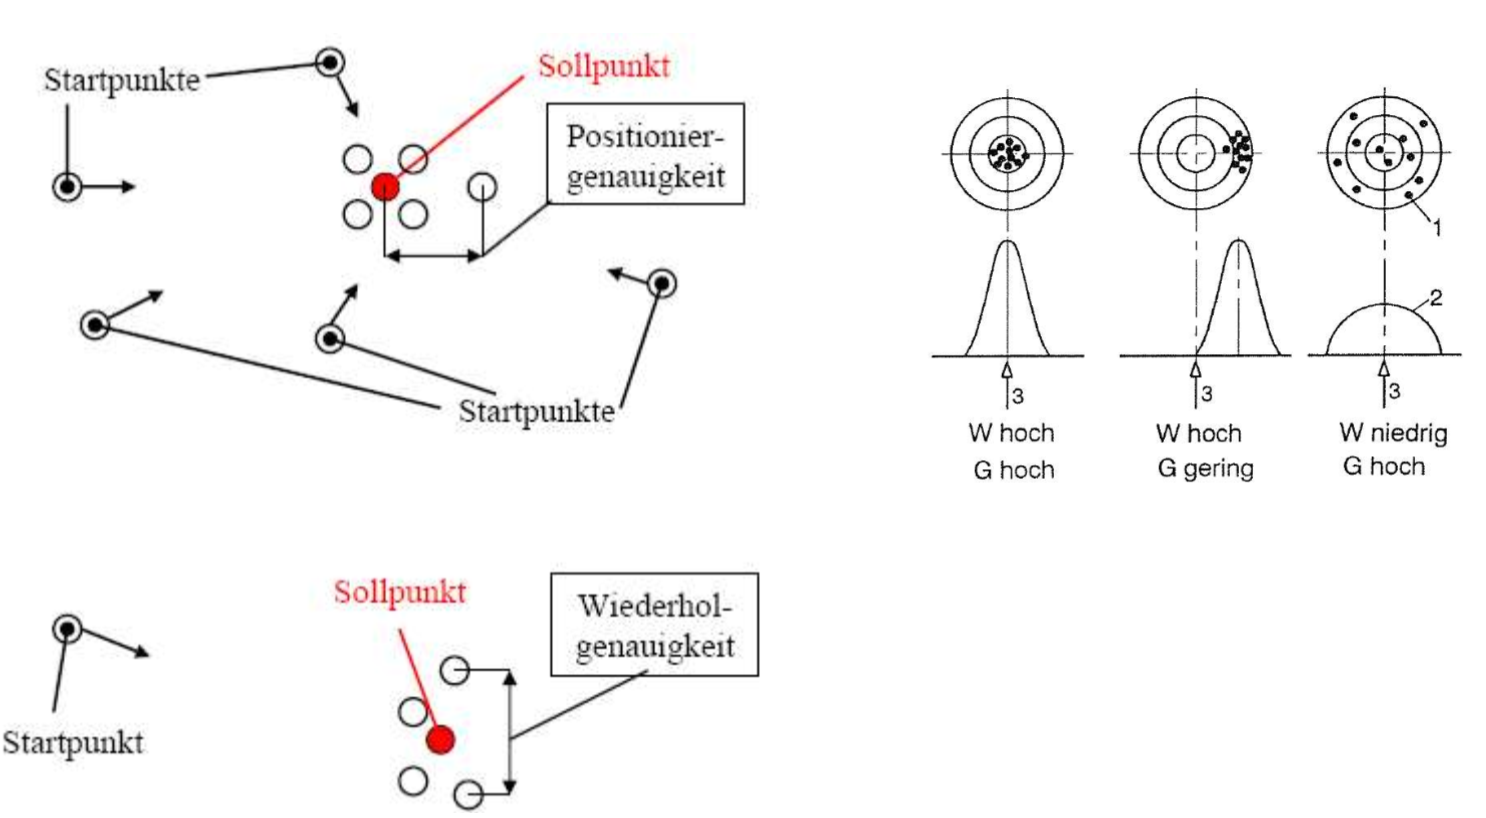
\includegraphics[width=\linewidth]{./bilder/genauigkeit.png}
\end{minipage}
\begin{minipage}{0.5\linewidth}
\subsection{Anforderungen}
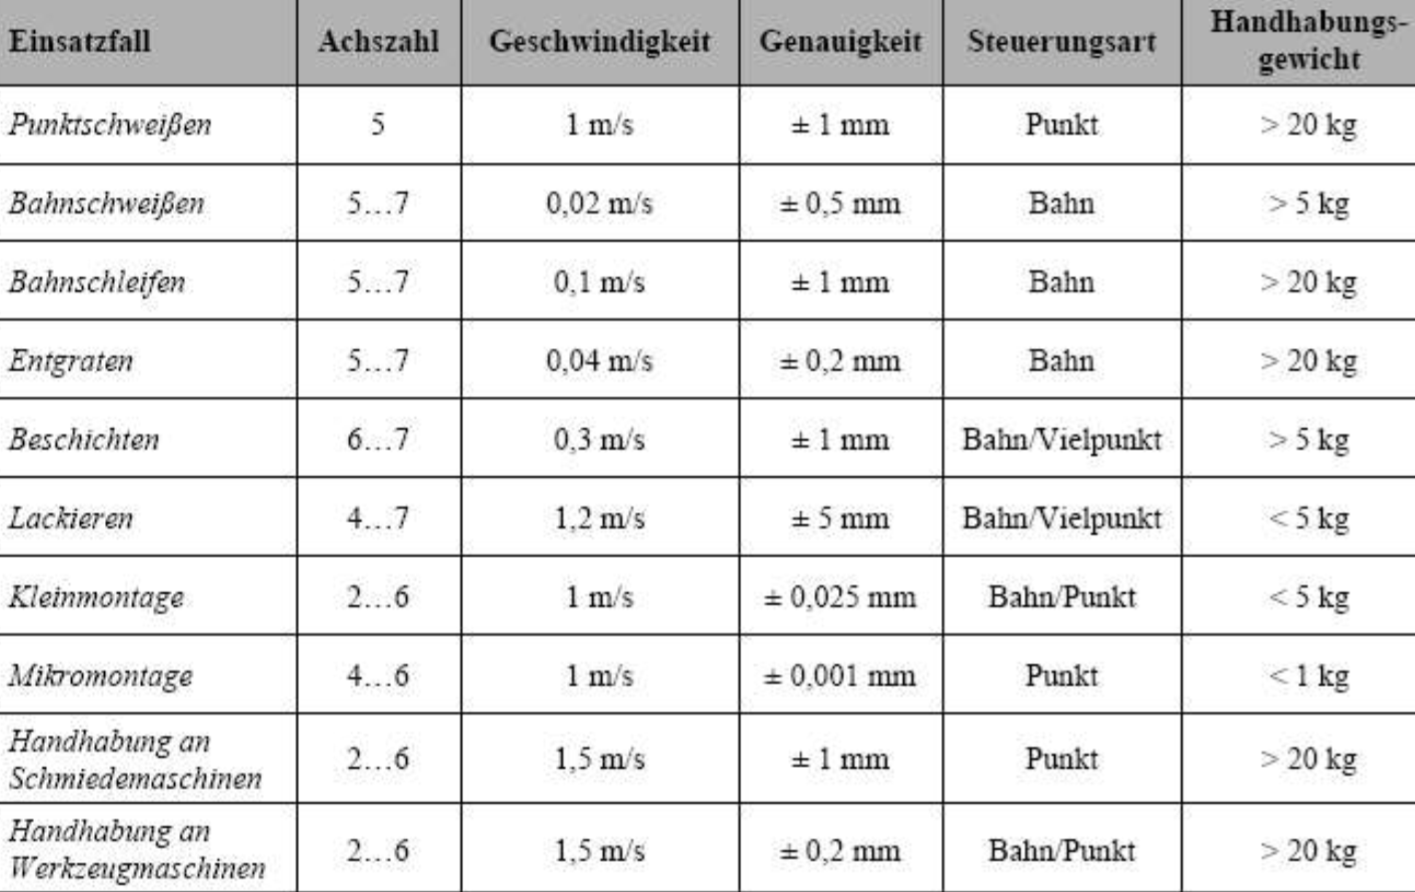
\includegraphics[width=\linewidth]{./bilder/anforderung.png}
\textbf{lösung übung 1 einfügen}
\end{minipage}

\begin{minipage}{0.5\linewidth}
    \subsection{Anlage}
    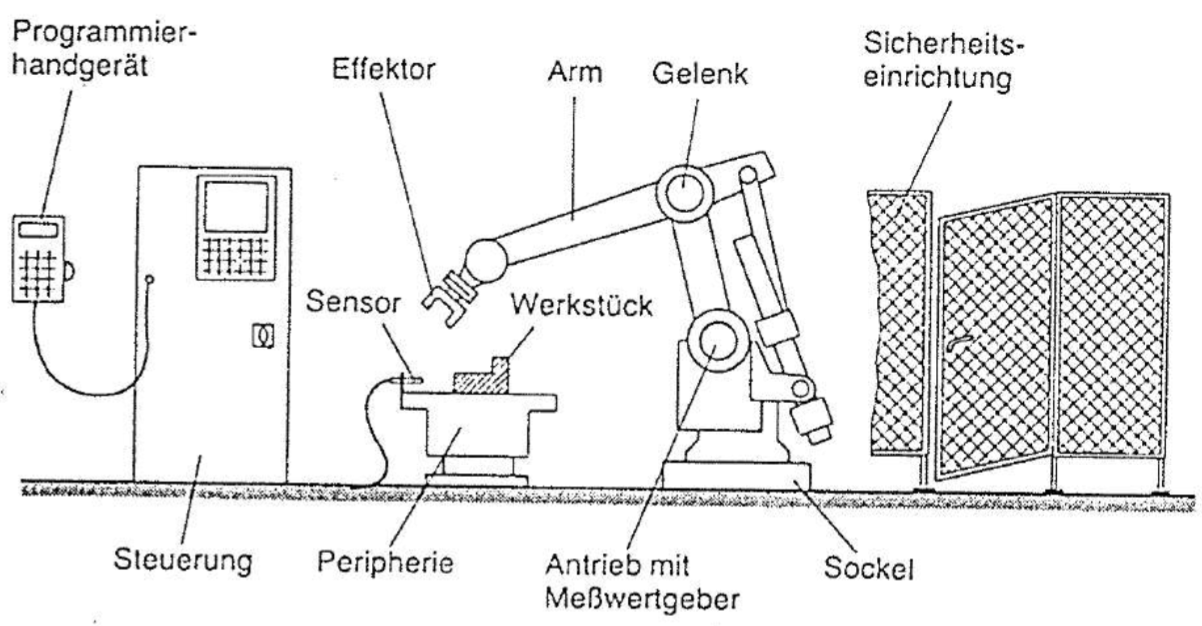
\includegraphics[width=\linewidth]{./bilder/anlage.png}
\end{minipage}
\begin{minipage}{0.5\linewidth}
    \subsection{Komponent}
    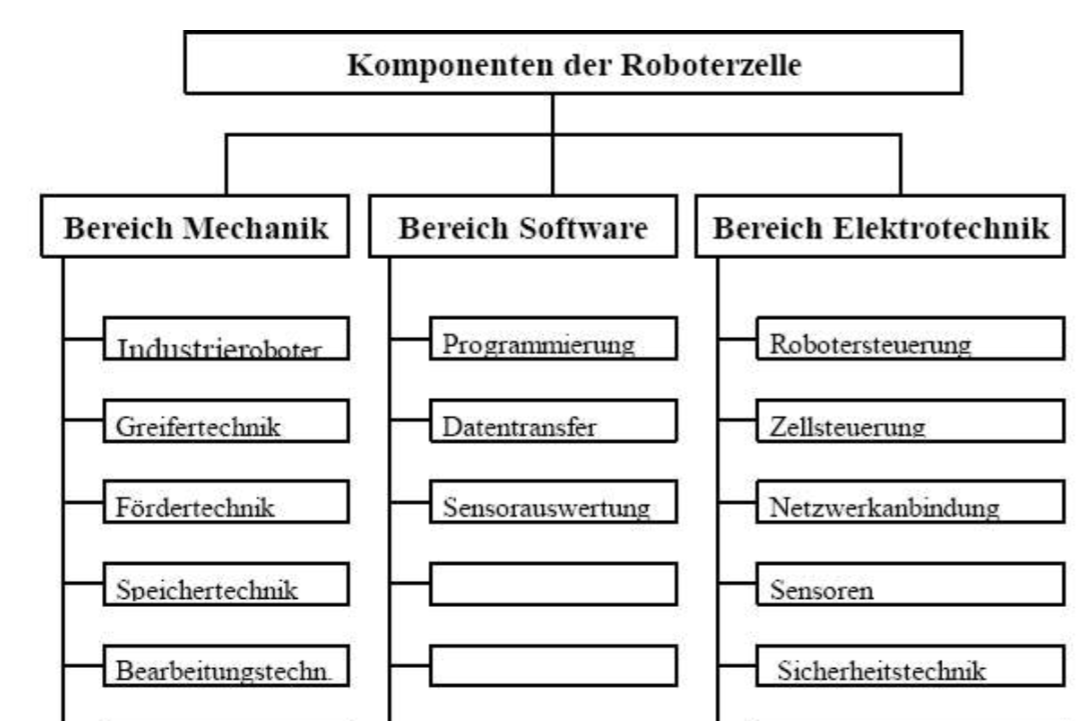
\includegraphics[width=\linewidth]{./bilder/komponent.png}
\end{minipage}
\subsection{Kinematik}
\begin{minipage}{0.5\linewidth}
\subsubsection{Seriell}
\begin{itemize}
    \item Das erste Armglied ist fest mit dem Boden/Sockel verbunden.
    \item Am letzten Armglied ist ein Effektor befestigt.
    \item An jedem Armgield befindet sich nur ein Gelenk, welches das nächste Armglied verbindet.  
\end{itemize}
\end{minipage}
\begin{minipage}{0.5\linewidth}
\subsubsection{Parallel}
\begin{itemize}
    \item mindestens einen geschlossenen kinematische Kette.
    \item entsteht, wenn ein Armteil auf zwei verschiedenen Wegen mit dem Sockel vebrunden ist.
\end{itemize}
\end{minipage}
\clearpage
\section{Mathematische Grundlagen der Robotik}

\subsection{TI-Nspire CX CAS Befehle}
Die Bibliothk findet sich im Repo \href{LMazzole/tinspire}{https://github.com/LMazzole/tinspire}\newline
\begin{tabular}{p{5cm}p{10cm}}

\texttt{$[ x_{11} , x_{12} ; x_{21},x_{22}]$} &  $ \begin{bmatrix}
            	x_{11} & x_{12}\\
            	x_{21} & x_{22}\\
            \end{bmatrix} $ \\
\texttt{ $[ \ldots]^{-1} $} & Inverse Matrix\\
\texttt{ $[ \ldots] $ (2ND CATALOG) \small{T} } & Transponierte Matrix
$[\ldots]^{T}$\\

\end{tabular} \\
	
%
%	\subsection{Matritzenrechnen}
%		\subsubsection{Vektoren im Raum}
%			$\vec{p}_{AB}=
%			\begin{matrix}
%            	x_B-x_A\\
%            	y_B-y_A\\
%            	z_B-z_A\\
%            \end{matrix}$\\
%			
%			Transponierung: $a^T\cdot b= \left(a_1 \vspace{0.2cm} a_2\vspace{0.2cm}  \ldots a_n \right) 
%			\cdot $
%	
%		\subsubsection{Matrizen Multiplikation \small{(A muss gleich viele Spalten
%		haben wie B Zeilen hat)}}
%		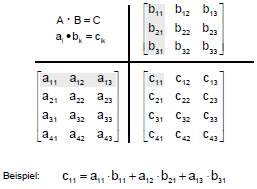
\includegraphics[width=7cm]{./bilder/matrizenmultiplikation.png}
%    	
%	
%	
%	
%\subsection{Übersicht}
%	\begin{tabular}{l l}
%    	Transponierte Matrix: & $A^T=[a_{ik}^T]=[a_{ki}]$ vertauschen der Zeilen
%    	mit Spalten\\
%    	Einheitsmatrix:& $I_n= 
%			    	\begin{bmatrix} 
%			        	1&0 & 0\\
%			        	0&1&0\\
%			        	0&0&1                               
%			        \end{bmatrix}$		    
%    \end{tabular}
%
\subsection{Determinante}
\begin{minipage}{9cm}
    
    	\textbf{2x2 Matrix}    
    $$ \det \begin{bmatrix} a_{11} & a_{12} \\
                            a_{21} & a_{22} \end{bmatrix} =
                            a_{11} a_{22} - a_{12} a_{21}  $$
\end{minipage}
\begin{minipage}{0.45\linewidth}
    	\textbf{3x3 Matrix}\newline
    $ \det \begin{bmatrix} a_{11} & a_{12} & a_{13} \\
    a_{21} & a_{22}& a_{23} \\
    a_{31} & a_{32} & a_{33} \end{bmatrix}
    $=\begin{minipage}{0.7\linewidth}
        $a_{11} a_{22} a_{33}
        + a_{12} a_{23} a_{31}
        + a_{13} a_{21} a_{32}$ \newline$
        - a_{13} a_{22} a_{31}
        - a_{12} a_{21} a_{33}
        - a_{11} a_{23} a_{32}  $
    \end{minipage} 
\end{minipage}	

%	
% 	\textbf{Dreiecksmatrix} - Alle Elemente entweder ober- oder unterhalt der Hauptdiagonale $= 0$
% 	$$\det A =a_{11}\cdot a_{22}\dotsb a_{nn} \quad  \quad \text{Die Det. ist das Produkt
% 	der Hauptdiagonal-Einträge. Gilt somit auch für Diagonalmatritzen.} $$
%% 	
%	\textbf{Null $(|A| = 0)$} - Wenn $A$ eine (n,n)-Matrix ist, so wird $|A| = 0$ unter einer der
%	folgenden Bedingungen:
%	\begin{itemize}
%    	\item Zwei Zeilen/Spalten sind linear abhängig (gleich oder ein Vielfaches der anderen).
%    	\item Alle Elemente einer Zeile/Spalte sind Null. \\
%  	\end{itemize} 
%	\clearpage
% 	\textbf{Allgemein:}
% 	$$A\epsilon M_n: \det A =    
% 	\begin{vmatrix}
%     	a_{11} & a_{12}& \ldots & a_{1n}\\
%     	a_{21}& &\ldots & \\
%     	\ldots \\
%     	a_{n1} & & \ldots & a_{nn}    			
%     \end{vmatrix}=
% 	(-1)^{1+1}a_{11}D_{11} + (-1)^{1+2}a_{12}D_{12}+ \ldots +
% 	(-1)^{1+n}a_{1n}D_{1n}$$
% 	
% 	\subsubsection{Unterdeterminante}
% 	$$D_{11}=
% 	\begin{vmatrix}
%     	a_{22} & \ldots & a_{2n}\\
%     	\ldots\\
%     	a_{n2}& \ldots & a_{nn}
%     \end{vmatrix} 	\\
% 	D_{12}=
% 	\begin{vmatrix}
%     	a_{21} & a_{23}& \ldots & a_{2n}\\
%     	\ldots\\
%     	a_{n1}& a_{n3}&\ldots & a_{nn}
%     \end{vmatrix}$$\\
% 	$D_{ij}$ die (n-1)$ \times $(n-1)-Untermatrix von D ist, die durch Streichen der
% 	i-ten Zeile und j-ten Spalte entsteht.\\
% 	Diese Methode ist zu empfehlen, wenn die Matrix in einer Zeile oder Spalte
% 	bis auf eine Stelle nur Nullen aufweisst.
% 	Dies lässt sich meist mit dem Gausverfahren bewerkstelligen.
% 	
% \subsection{Gaussverfahren}
% 	Durch Addition und Subtraktion einzelner Zeilen (auch von Vielfachen einer
% 	Zeile) werden einzelne Stellen auf Null gebracht. zB:\\
% 	$\begin{bmatrix}
%     	a_{11} & a_{12}& \ldots & a_{1n}\\
%     	a_{21}& &\ldots & \\
%     	\ldots \\
%     	a_{n1} & & \ldots & a_{nn}    			
%     \end{bmatrix}=
% 	\begin{bmatrix}
%     	a_{11} & a_{12}& \ldots & a_{1n}\\
%     	k a_{21}-n a_{11}& ka_{22}-n a_{12}&\ldots & k a_{2n} - n a_{1n}\\
%     	\ldots \\
%     	a_{n1} & & \ldots & a_{nn}    			
%     \end{bmatrix}$ \\
% 	Die n * erste Zeile wurde von der k * zweiten Zeile abgezogen ($a_{2.}= 
% 	k a_{2.}- n a_{1.}$) 
	
\subsection{Inverse Matrix}
Existiert nur wenn Matrix regulär: $\det A \neq 0$\newline
\begin{minipage}{9cm}
	\textbf{2x2 Matrix}
	$$ A^{-1} = \begin{bmatrix} a & b \\ c & d \\ \end{bmatrix}^{-1} = \frac{1}{ad
	- bc} \begin{bmatrix} d & -b \\ -c & a \\ \end{bmatrix} $$
\end{minipage}
\begin{minipage}{11cm}
	\textbf{3x3 Matrix}\newline
  $  A^{-1} = \begin{bmatrix} a & b & c\\ d & e & f \\ g & h & i \\ \end{bmatrix}^{-1} =
  \frac{1}{\det(A)} \begin{bmatrix} ei - fh & ch - bi & bf - ce \\ fg - di & ai
  - cg & cd - af \\ dh - eg & bg - ah & ae - bd \end{bmatrix} $
\end{minipage}\\

% \textbf{Diagonalmatrix} (Alle Elemente ausserhalb der Hauptdiagonale $= 0$, Elemente auf
% Hauptdiagonale sind Eigenwerte $\lambda_i$): \\ 
% Alle Elemete elementweise invertieren - Kehrwert. $\quad \Rightarrow \quad $\textit{Gilt nur wenn
% alle Elemente auf der Hauptdiagonale $\neq 0$ sind.}\\
% 
% \textbf{Allgemein:}\\
% 	$A^{-1}= \begin{bmatrix}
%     	a_{11} & a_{12}& \ldots & a_{1n}\\
%     	a_{21}& &\ldots & \\
%     	\ldots \\
%     	a_{n1} & & \ldots & a_{nn}    			
%     \end{bmatrix}^{-1}$
% 	\begin{enumerate}
% 		\item $A^T$ bestimmen (Zeilen und Spalten vertauschen) $A^{T}= \begin{bmatrix}
%     	a_{11} & a_{21}& \ldots & a_{n1}\\
%     	a_{12}& &\ldots & \\
%     	\ldots \\
%     	a_{1n} & & \ldots & a_{nn}    			
%     \end{bmatrix}$	
% 		\item Bei $A^T$ jedes Element $a_{ij}$ durch Unterdet. $D_{ij}$ mit
% 		richtigem Vorzeichen ersetzen $A^*=	\begin{bmatrix}
% 			(-1)^{1+1}D_{11} &  \ldots	& (-1)^{1+n} D_{1n}\\
% 			\ldots\\
% 			(-1)^{n+1} D_{n1}& \ldots  & (-1)^{n+n} D_{nn}
% 		\end{bmatrix}$
% 		\item $A^{-1} = \frac{A^*}{\det A}$ 
%     \end{enumerate}
%  
%  \subsection{Diagonalisierung}
%  	\begin{enumerate}
%        \item Eigenwerte $\lambda$ auschrechnen: $\det (A - I_n \lambda)=0$
%        \item Eigenvektoren $\vec{v}$ bilden: $(A- \lambda I_n)\vec{v}=0$
%        \item Transformationsmatrix: $T= [\vec{v_1} \ldots \vec{v_n}]$
%        \item $T^{-1}$ berechnen (Achtung ist A symmetrisch, dh. $A^T=A$ und
%        oder alle EV senktrecht zueinander, dann $T^{-1}=T^T$)
%        \item $D=\begin{bmatrix}
%                 	\lambda_1 &0 &0\\
%                 	0& \lambda_2 &0\\
%                 	0& 0& \lambda_3
%                 \end{bmatrix}$
% 		\item $A^n = T D^n T^{-1}$
% 
%      \end{enumerate}
\subsection{Basis Rotationsmatrizen}
Der Winkel ist Positiv bei einer Rotation im Gegenuhrzeigersinn $ \circlearrowleft $\newline
	\begin{minipage}{0.33\linewidth}
		Rotation um x-Achse mit Winkel $\gamma$ \\
   		$R_x(\gamma)=\begin{bmatrix}
                		1 &0 &0\\
                		0 &cos(\gamma) &-sin(\gamma)\\
                		0 &sin(\gamma) &cos(\gamma)
                	 \end{bmatrix}$
    \end{minipage}
	\begin{minipage}{0.33\linewidth}
    	Rotation um y-Achse mit Winkel $\beta$\\
   		$R_y(\beta)=\begin{bmatrix}
                		cos(\beta) &0 &sin(\beta)\\
                		0 &1 &0\\
                		-sin(\beta) &0 &cos(\beta)
                	 \end{bmatrix}$
    \end{minipage}
	\begin{minipage}{0.33\linewidth}
    	Rotation um z-Achse mit Winkel $\alpha$ \\
   		$R_z(\alpha)=\begin{bmatrix}
                		cos(\alpha) &-sin(\alpha) &0\\
                		sin(\alpha) &cos(\alpha) &0\\
                		0 &0 &1
                	 \end{bmatrix}$
    \end{minipage}
\subsection{Aufeinanderfolgende Rotationen}
3 Koordinatensysteme \{A\}, \{B\}, \{C\} mit gleichem Ursprung\\ \\
\begin{minipage}{6cm}
    \textbf{Körperfestkoordinatensystem}\\
    "`An der Achse"'\\
    ${}^B\mathrm{p}={}^B_C\mathrm{R}\cdot{}^C\mathrm{p}$\\
    ${}^A\mathrm{p}={}^A_B\mathrm{R}\cdot{}^B\mathrm{p}$\\
    ${}^A\mathrm{p}={}^A_C\mathrm{R}\cdot{}^C\mathrm{p}$\\ \\
    ${}^A_C\mathrm{R}=\overrightarrow{{}^A_B\mathrm{R} \cdot {}^B_C\mathrm{R}}$\\
\end{minipage}
\begin{minipage}{6cm}
    \textbf{Raumfestkoordinatensystem}\\ 
    "`An der Welt oder Basis"'\\
    ${}^B\mathrm{p}={}^B_A\mathrm{R}{}^B_C\mathrm{R}{}^A_C\mathrm{R}\cdot{}^C\mathrm{p}$\\
    ${}^A\mathrm{p}={}^A_B\mathrm{R}\cdot{}^B\mathrm{p}$\\
    ${}^A\mathrm{p}={}^A_C\mathrm{R}\cdot{}^C\mathrm{p}$\\ \\
    ${}^A_C\mathrm{R}=\overleftarrow{{}^B_C\mathrm{R} \cdot {}^A_B\mathrm{R}}$\\
\end{minipage}   

\subsubsection{Punkte in verschiedenen Koordinatensystemen \robo{36}{2.1.6}}
\begin{tabular}{ll}
    \textbf{Translation}&${}^A\mathrm{P} = {}^A\mathrm{P}_{OB}+{}^B\mathrm{P} $ \\
    \textbf{Rotation} & ${}^A\mathrm{P} = {}^A_B\mathrm{R}\cdot {}^B\mathrm{P} $\\
    \textbf{Rotation + Translation}&$ {}^A\mathrm{P} = {}^A\mathrm{P}_{OB} +{}^A_B\mathrm{R}\cdot {}^B\mathrm{P} $\\
\end{tabular}
\clearpage


\subsection{Konvention Arctan2 \robo{42}{2.1.8}}
	\begin{minipage}{10cm}
    	$\theta=\arctan2(y,x)\Longrightarrow\left\{
    	\begin{array}{l}
            \text{1:\space\space}\theta=\arctan(\frac{y}{x})\\
			\text{2:\space\space}\theta=\pi+\arctan(\frac{y}{x})\\
			\text{3:\space\space}\theta=-\pi+\arctan(\frac{y}{x})\\
			\text{4:\space\space}\theta=-\arctan(\frac{y}{x})\\
		\end{array}\right.$
    \end{minipage}
	\begin{minipage}{10cm}
    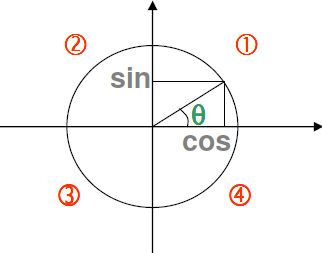
\includegraphics[width=4cm]{./bilder/einheitskreis.png}
    \end{minipage}

	\begin{minipage}{5cm}
    	\vspace{9mm}
    	$\theta=arctan2(\overbrace{y}^{sin(\theta)},\overbrace{x}^{cos(\theta)}) \Leftrightarrow$
    \end{minipage}
	\begin{minipage}[t]{0.8cm}
    	\textcircled{1}\\
    	\textcircled{2}\\
    	\textcircled{3}\\
    	\textcircled{4}
    \end{minipage}
	\begin{minipage}[t]{3.5cm}
    	$\theta= arctan(\frac{y}{x})$\\
    	$\theta= \pi + arctan(\frac{y}{x})$\\
    	$\theta= -\pi + arctan(\frac{y}{x})$\\
    	$\theta= -arctan(\frac{y}{x})$\\
    \end{minipage}
	\begin{minipage}[t]{2.5cm}
    	\hspace{2mm} $0 \leq \theta \leq \frac{\pi}{2}$\\
    	\hspace*{1.5mm} $\frac{\pi}{2} \leq \theta \leq \pi$\\
    	$-\pi \leq \theta \leq -\frac{\pi}{2}$\\
    	$-\frac{\pi}{2} \leq \theta \leq 0$
    \end{minipage}
	\begin{minipage}[t]{2.5cm}
    	für $+y$, $+x$\\
    	für $+y$, $-x$\\
    	für $-y$, $-x$\\
    	für $-y$, $+x$
    \end{minipage}
	\begin{minipage}[t]{4cm}
     	\begin{tabular}[t]{|l}
    	$\theta = \frac{\pi}{2}$ für $x=0$, $y>0$\\
    	$\theta = - \frac{\pi}{2}$ für $x=0$, $y<0$\\
    	$\theta = 0$ für $x=0$, $y=0$\\
    	\end{tabular}
    \end{minipage}

Ti Nspire CX CAS: \texttt{$ lm\backslash arctan2(Y,X)$}
\clearpage

\subsection{Rücktransformation auf Winkel}
	\begin{minipage}{9.5cm}
    \subsubsection{Z-Y-X Euler Winkel \robo{42}{2.1.8}}
    \begin{tabular}{|p{2.5cm}|p{6cm}|}
        \hline
        \multicolumn{2}{|l|}{Körperfest Koordinatensystem}\\
        \hline
        Vorgehen&
        \vspace{-0.3cm}
        \begin{enumerate}
            \item Drehen um Z mit Winkel $\alpha$
            \item Drehung um Y' mit Winkel $\beta$
            \item Drehung um X'' mit Winkel $\gamma$\vspace{-0.5cm}
        \end{enumerate}\\
        \hline
        Rotationsmat.:
        & ${^A_B}R(\overrightarrow{\alpha,\beta,\gamma}) = 
        \begin{bmatrix} 
        r_{11} & r_{12} & r_{13} \\
        r_{21} & r_{22} & r_{23} \\
        r_{31} & r_{32} & r_{33}                              
        \end{bmatrix}$ \\
        \hline
        \multicolumn{2}{|l|}{{\footnotesize 
                $ \overrightarrow{R_Z(\alpha)\cdot R_{Y'}(\beta) \cdot R_{X''}(\gamma)}$= $\begin{bmatrix} 
                c\alpha c\beta & c\alpha s\beta s\gamma - s\alpha c\gamma & c\alpha s\beta c\gamma + s\alpha s\gamma \\
                c\alpha c\beta & s\alpha s\beta s\gamma + c\alpha c\gamma & s\alpha s\beta c\gamma - c\alpha s\gamma \\
                -s\beta & c\beta s\gamma & c\beta c\gamma                            
                \end{bmatrix}$
        }}\\\hline 
        \multicolumn{2}{|l|}{\textbf{Rücktransformation}}\\
        \hline
			Ansatz:
& $cos(\beta) = \sqrt{r^2_{11} + r^2_{21}}$ \\
& $sin(\beta) = -r_{31}$\\
\hline
Winkel:
& $\beta=arctan2(-r_{31},\sqrt{r^2_{11}+r^2_{21}})$\\
$cos(\beta) \neq 0 $ &$\alpha=arctan2(\frac{r_{21}}{cos\beta},\frac{r_{11}}{cos\beta})$\\
& $\gamma=arctan2(\frac{r_{32}}{cos\beta},\frac{r_{33}}{cos\beta})$\\
\hline
$\beta=\frac{\pi}{2}$:
& $\alpha=0,\gamma=arctan2(r_{12},r_{22})$\\
$\beta=-\frac{\pi}{2}$:
& $\alpha=0,\gamma=-arctan2(r_{12},r_{22})$\\
\hline
        
    \end{tabular}
    
    
    
\end{minipage}
\begin{minipage}{9.5cm}
    \subsubsection{X-Y-Z Roll-Nick-Gier Winkel}
   	\begin{tabular}{|p{2.5cm}|p{6cm}|}
    \hline
   
      	\multicolumn{2}{|l|}{Raumfestes Koordinatensystem}\\        	
    \hline
    Vorgehen&
    \vspace{-0.3cm}
    \begin{enumerate}
        \item Drehung um $X_A$ mit Winkel $\gamma$
        \item Drehung um $Y_A$ mit Winkel $\beta$
        \item Drehung um $Z_A$ mit Winkel $\alpha$\vspace{-0.5cm}
    \end{enumerate}\\ \hline
   		Rotationsmat.:
   		& ${^A_B}R(\overleftarrow{\alpha,\beta,\gamma}) = 
   			\begin{bmatrix} 
		    	r_{11} & r_{12} & r_{13} \\
       r_{21} & r_{22} & r_{23} \\
       r_{31} & r_{32} & r_{33}                              
   \end{bmatrix}$ \\
            \hline               
          \multicolumn{2}{|l|}{{\footnotesize 
              $ \overleftarrow{R_Z(\alpha)\cdot R_Y(\beta) \cdot R_X(\gamma)}$= $\begin{bmatrix} 
                c\alpha c\beta & c\alpha s\beta s\gamma - s\alpha c\gamma & c\alpha s\beta c\gamma + s\alpha s\gamma \\
                c\alpha c\beta & s\alpha s\beta s\gamma + c\alpha c\gamma & s\alpha s\beta c\gamma - c\alpha s\gamma \\
                -s\beta & c\beta s\gamma & c\beta c\gamma                            
            \end{bmatrix}$
        }}\\
	\hline     
       	\multicolumn{2}{|l|}{\textbf{Rücktransformation}}\\ \hline 
        \multicolumn{2}{|l|}{Gleich wie Z-Y-X} \\ \hline    
    \end{tabular}
   	\vspace{4.4cm}
\end{minipage}
    
\begin{minipage}{9.5cm}
    \vspace{0.5cm}
    \subsubsection{Z-Y-Z Euler Winkel \robo{39}{2.1.8}}
   	\begin{tabular}{|p{2.5cm}|p{6cm}|}
    \hline
       	\multicolumn{2}{|l|}{Körperfestes Koordinatensystem}\\  	
    \hline
    Vorgehen&
    \vspace{-0.3cm}
    \begin{enumerate}
        \item Drehen um Z mit Winkel $\alpha$
        \item Drehung um Y' mit Winkel $\beta$
        \item Drehung um Z'' mit Winkel $\gamma$\vspace{-0.5cm}
    \end{enumerate}\\
    \hline
       	Rotationsmat.:
   		& ${^A_B}R(\overrightarrow{\alpha,\beta,\gamma}) = 
   			\begin{bmatrix} 
		    	r_{11} & r_{12} & r_{13} \\
       r_{21} & r_{22} & r_{23} \\
       r_{31} & r_{32} & r_{33}                              
   \end{bmatrix}$ \\
	\hline
        \multicolumn{2}{|l|}{{\scriptsize 
        $ \overrightarrow{R_Z(\alpha)\cdot R_{Y'}(\beta) \cdot R_{Z''}(\gamma)}$= $\begin{bmatrix} 
           c\alpha c\beta c\gamma - s \alpha s \gamma &-c\alpha c\beta s\gamma-s\alpha c\gamma &c\alpha s\beta \\
           s\alpha c\beta c\gamma + c \alpha s \gamma& -s\alpha c\beta s\gamma+c\alpha c\gamma & s\alpha s\beta\\
           -s\beta c\gamma& s\beta s\gamma& c\beta
        \end{bmatrix}$
    }}\\\hline 
		Ansatz:
		& $sin(\beta) = \sqrt{r^2_{31} + r^2_{32}}$ \\
		& $cos(\beta) = r_{33}$\\
	\hline
		Winkel:
		& $\beta=arctan2(\sqrt{r^2_{31}+r^2_{32}},r_{33})$\\
		$ sin(\beta) \neq 0 $& $\alpha=arctan2(\frac{r_{23}}{sin\beta},\frac{r_{13}}{sin\beta})$\\
		& $\gamma=arctan2(\frac{r_{32}}{sin\beta},-\frac{r_{31}}{sin\beta})$\\
	\hline
		$\beta=0$:
		& $\alpha=0,\gamma=arctan2(-r_{12},r_{11})$\\
		$\beta=\pi$:
		& $\alpha=0,\gamma=arctan2(r_{12},-r_{11})$\\
	\hline
    \end{tabular} 	
\end{minipage}
	
\clearpage


 \subsection{Transformations Matrix}
 \subsubsection{Aufbau}
 \begin{minipage}{10cm}
     Transformationsmatrix: T = $ 
     \begin{bmatrix} 
     r_{11} & r_{12} & r_{13} & x_{ab} \\
     r_{21} & r_{22} & r_{23} & y_{ab} \\
     r_{21} & r_{22} & r_{23} & z_{ab} \\
     0 & 0 & 0 & x                              
     \end{bmatrix}$
     
     x = 1 bei Ortsvektor \hspace{1cm} x = 0 bei Feiem Vektor
     
 \end{minipage}
 \begin{minipage}{0.33\linewidth}
     \textbf{Translation}\newline
     $Trans(a,b,c)=\begin{bmatrix}
     1 & 0 & 0 & a \\ 
     0 & 1 & 0 & b \\ 
     0 & 0 & 1 & c \\ 
     0 & 0 & 0 &  1
     \end{bmatrix}$
 \end{minipage}
 
 
 \begin{minipage}{0.33\linewidth}
     \textbf{Rotation um x-Achse mit Winkel $ \gamma$}\newline
     $ Rot_x(\gamma)=\begin{bmatrix}
     1 & 0 & 0 & 0 \\ 
     0 & cos(\gamma) & -sin(\gamma) & 0 \\ 
     0 & sin(\gamma) & cos(\gamma) & 0 \\ 
     0 & 0 & 0 & 1
     \end{bmatrix}$
 \end{minipage}    
 \begin{minipage}{0.33\linewidth}
     \textbf{Rotation um y-Achse mit Winkel $ \beta$}\newline
     $ Rot_y(\beta)=\begin{bmatrix}
     cos(\beta)& 0  & sin(\beta)  & 0  \\ 
     0 & 1 & 0 & 0  \\ 
     -sin(\beta)&  0 & cos(\beta) & 0 \\ 
     0 & 0 & 0  & 1
     \end{bmatrix}$
 \end{minipage}
 \begin{minipage}{0.33\linewidth}
     \textbf{Rotation um z-Achse mit Winkel $\alpha$}\newline
     $Rot_z(\alpha)=\begin{bmatrix}
     cos(\alpha)& -sin(\alpha) & 0 & 0 \\ 
     sin(\alpha)&  cos(\alpha)& 0 & 0 \\ 
     0 & 0 & 1 & 0 \\ 
     0 & 0 & 0 & 1
     \end{bmatrix} $
 \end{minipage} 
 
 \subsubsection{Multiplikation \robo{36}{2.1.6}}
 Transformations Matrix über mehrere Koordinatensysteme:\\
 
 ${}^0_n\mathrm{T}={}^0_1\mathrm{T}\cdot{}^1_2\mathrm{T}\cdot{}$\ldots$\cdot{}^{n-1}_n\mathrm{T}$;
 \space\space\space\space ${}^A_B\mathrm{T} \Rightarrow$
 Transformationsmatrix von Koordinatensystem A nach B
 
 \subsubsection{Punkte in verschiedenen Koordinatensystemen \robo{36}{2.1.6}}
 ${}^B\mathrm{P}={}^B_A\mathrm{T}\cdot{}^A\mathrm{P}$ \\ \\
 ${}^A\mathrm{P}={}^A_B\mathrm{T}\cdot{}^B\mathrm{P}=({}^B_A\mathrm{T})^{-1}\cdot{}^B\mathrm{P}$
 
 \subsubsection{Distanz eines Vektors}
 Distanz$\begin{bmatrix}
 x\\
 y\\
 z\\
 1
 \end{bmatrix}\rightarrow$d=$\sqrt{x^2+y^2+z^2}$
\clearpage
\section{Koordinaten Transformation \robo{37}{3}}
\begin{minipage}{0.5\linewidth}
    \subsection{Transformation}
    \begin{minipage}{0.39\linewidth}
        \textbf{Gelenkkoord.}\newline
        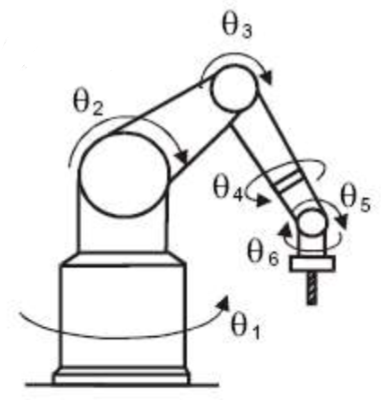
\includegraphics[height=3cm]{./bilder/koordtrans1}
    \end{minipage}
    \begin{minipage}{0.19\linewidth}  
          
        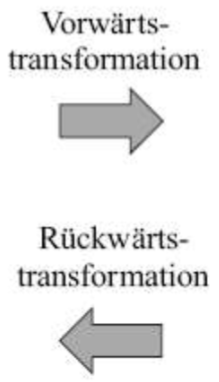
\includegraphics[height=3cm]{bilder/koordtrans2}
    \end{minipage}
    \begin{minipage}{0.39\linewidth}
        \textbf{Globale kart. Koord.}\newline
        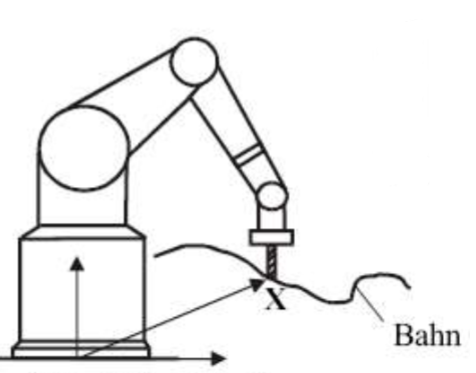
\includegraphics[height=3cm]{./bilder/koordtrans3}
    \end{minipage}
\end{minipage}
\begin{minipage}{0.5\linewidth}
\subsection{Koordinatensysteme}
\begin{tabular}{|c|c|}
    \hline
    Auf Greifer (TCP) & Auf Werkstück\\
    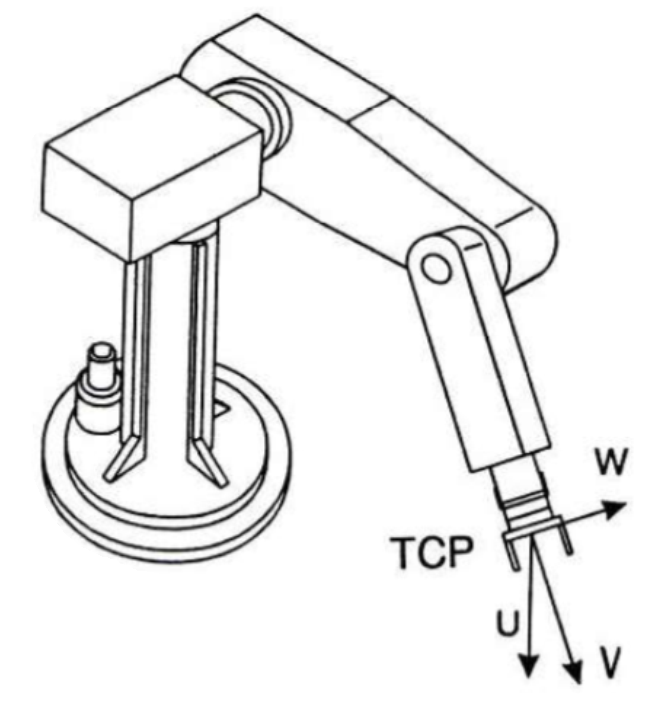
\includegraphics[height=3cm]{./bilder/koordsys1a} & 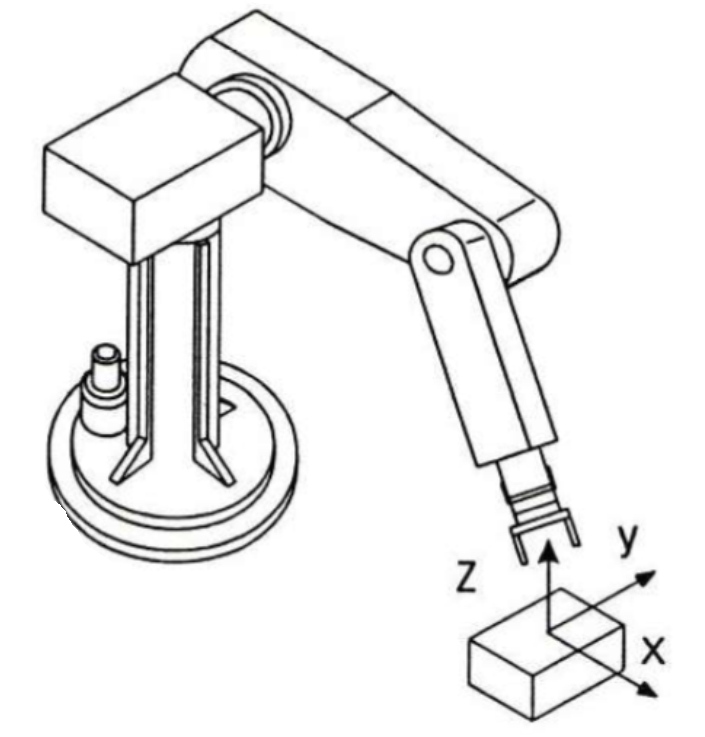
\includegraphics[height=3cm]{./bilder/koordsys1b}\\
    \hline
    Auf Drehaschse 1-6 & Auf Fusspunkt (Raumfest)\\
        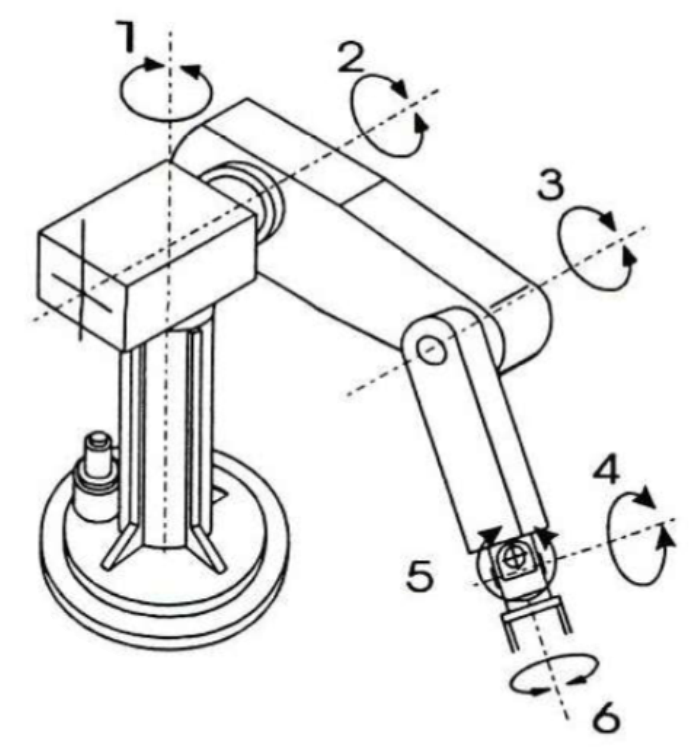
\includegraphics[height=3cm]{./bilder/koordsys1c} & 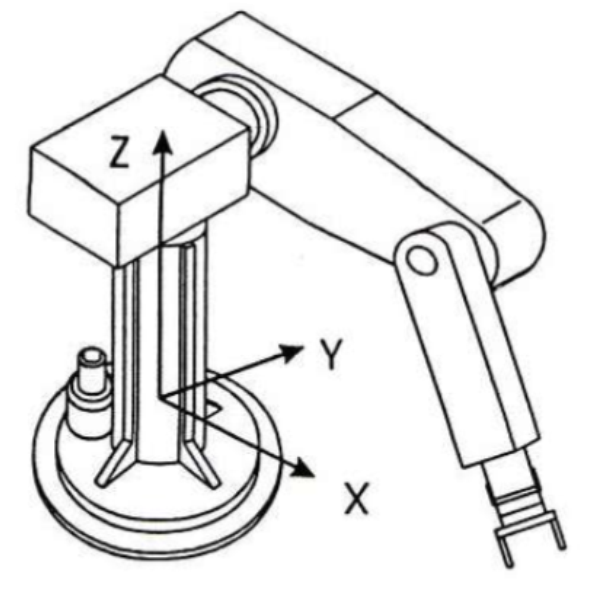
\includegraphics[height=3cm]{./bilder/koordsys1d}\\
    \hline
\end{tabular}
\end{minipage}
\begin{multicols}{2}
    \begin{minipage}{\linewidth}
        \subsubsection{Gelenkkoordinaten}
        \vspace{-1cm}
        \[ q=\begin{bmatrix}
        q_1\\
        q_2\\
        \vdots\\
        q_n
        \end{bmatrix} \]
        \begin{tabular}{ll}
            $q_i = \theta_i$ & Winkel für Drehgelenke\\
            $q_i = d_i$& Verschiebung für Schubgelenke\\
        \end{tabular}
    \end{minipage}

    \begin{minipage}{\linewidth}
        \subsubsection{Kartesische Koordinaten}
        \vspace{-1cm}
        \[ X= \begin{bmatrix}
            {}^0 P_{T_x}\\
            {}^0 P_{T_y}\\
            {}^0 P_{T_z}\\
            \alpha\\
            \beta\\
            \gamma
            \end{bmatrix}           
    \begin{array}{@{\kern-\nulldelimiterspace}l@{}}
          \left.\begin{array}{@{}c@{}}
              \vphantom{\vdots}\\
              \vphantom{\vdots}\\
              \vphantom{\vdots}
          \end{array}\right\}
          \parbox{20em}{Position des Ursprungs von \{T\} in \{O\}\\
          $\rightarrow$Beschreibt die Lage des TCP }\\
          \left.\begin{array}{@{}c@{}}
              \vphantom{\vdots}\\
              \vphantom{\vdots}\\
              \vphantom{\vdots}
          \end{array}\right\}\parbox{20em}{z.B. Euler Winkel\\
              $\rightarrow$Beschreibt die Orientierung des Greifers }\\
      \end{array}
        \]
    \end{minipage}
\end{multicols}
\subsubsection{Vorwärtstransformation \robo{58}{3.1}}
\subsubsection{Rückwärtstransformation \robo{58}{3.2}}
\clearpage
\subsection{Denavit-Hartenberg \robo{46}{2.2}}
\begin{minipage}{19cm}
    \textbf{Ablauf:}
    \begin{enumerate}{\setlength{\itemsep}{0cm}\setlength{\parsep}{0cm} \setlength{\topsep}{0cm}}
        \item Gelenke nummerieren in aufsteigender Reihenfolge, inkl. Effektor. Starten in der Basis mit Nummer null.
        \item Jeden Achskörper mit Koordinatensystem belegen.
        \item Die $z_i$-Koordinatenachse muss mit der i+1 Gelenkachse zusammenfallen.
        \item Die $x_i$-Achse liegt entlang der Normalen zwischen der $z_{i-1}$ und $z_i$-Achse und zeigt vom Gelenk i zum Gelenk i+1.
        \item $y_i$-Achsen vervollständigen mit der Rechten-Hand-Regel. (x:Daumen, y:Zeigfinger, z:Mittelfinger)
        \item Festlegen der DH-Parameter (siehe DH-Parameter) und eintragen in DH-Tabelle.
        \item DH-Matrizen berechnen und miteinander mulitplizieren.
    \end{enumerate}
    \vspace{0.2cm}
\end{minipage}\\

\begin{minipage}{19cm}
    \textbf{Anmerkung Koordinatensysteme:}
    \begin{itemize}\itemsep0pt
        \item $z_i$-Achse muss grundsätzlich mit Bewegungsachse des zugehörigen Achskörper zusammenfallen.
        Bei Rotationsgelenken gilt die Rechte-Handregel für Drehungen. 
        \item Ursprung des Koordinatensystems im Schnittpunkt der Bewegungsachsen.
    \end{itemize}
    \vspace{0.2cm}
\end{minipage}\\

\begin{minipage}{19cm}
    \textbf{DH-Parameter:}\\ \\
    \begin{tabular}{l l}
        Linklänge $a_i$ (Fixwert): 				& Für $z_{i-1}$ und $z_i$ Achse wird die gem. Normale mit Länge $a_i$ in $x_i$-Richtung gemessen.\\
        Linkdrehung $\alpha_{i}$ (Fixwert):		& Drehwinkel um $x_i$-Achse bis $z_{i-1}$- und $z_i$-Achse in gleiche Richtung zeigen.\\
        Link Offset $d_i$ (Variable):			& Abstand von $x_{i-1}$- und $x_i$-Achse entlang der $z_{i-1}$-Achse.\\
        Gelenkwinkel $\theta_{i}$ (Variable):	& Drehwinkel um $z_{i-1}$-Achse bis $x_{i-1}$- und $x_i$-Achse in gleiche Richtung zeigen.\\
    \end{tabular}
    \vspace{0.5cm}
\end{minipage}\\
\begin{minipage}{19cm}
    \textbf{DH-Tabelle:}\\ \\
    \begin{minipage}{10cm}
        \renewcommand{\arraystretch}{1.1}
        \begin{tabular}{| c | c | c | c | c |}
            \hline
            \textbf{Gelenk Nr.}
            & \textbf{Linklänge $a_i$}
            & \textbf{Linkdrehung $\alpha_{i}$}
            & \textbf{Link Offset $d_i$} 
            & \textbf{Gelenkwinkel $\theta_{i}$}\\
            \hline
            i =1
            &&&& \\
            \hline
            i+1
            &&&& \\
            \hline
            \ldots
            &&&&\\
            \hline
        \end{tabular}
        \renewcommand{\arraystretch}{1}
        \vspace{0.5cm}
    \end{minipage}
\end{minipage}\\
\begin{minipage}{19cm}
    \textbf{DH-Matrizen: \robo{52}{2.2.3}}\\ \\
    $ ^{i-1}_{i}T =
    \begin{bmatrix}
    cos(\theta_i) & -sin(\theta_i) cos(\alpha_i) &  sin(\theta_i) sin(\alpha_i) & a_i cos(\theta_i)\\
    sin(\theta_i) &  cos(\theta_i) cos(\alpha_i) & -cos(\theta_i) sin(\alpha_i) & a_i sin(\theta_i)\\
    0			  &  sin(\alpha_i)				 &  cos(\alpha_i)				& d_i\\
    0			  &  0							 &  0							& 1\\
    \end{bmatrix}
    \qquad
    ^{0}_{n}T = \prod\limits_{i=1}^{n} \quad ^{i-1}_{i}T(\theta_{i}) = ^{0}_{1}T \cdot ^{1}_{2}T \cdot \ldots \cdot ^{n-1}_{n}T $
\end{minipage}\\

\begin{minipage}{3cm}
    \textbf{Beispiel:}
    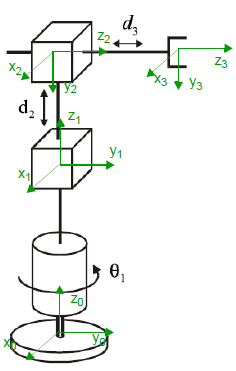
\includegraphics[width=4cm]{./bilder/denavitgrafik} \\
\end{minipage}
\begin{minipage}{6cm}
    $\alpha_{i} \Longrightarrow $ Linkdrehung  \\
    $ a_{i} \Longrightarrow $ Linklänge [Achsenabstand] \\
    $ d_{i} \Longrightarrow $ Offset \\
    $ \Theta_{i} \Longrightarrow $ Gelenkwinkel \\ 
\end{minipage}
\begin{minipage}{8cm}
    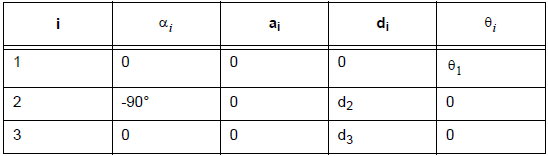
\includegraphics[width=9cm]{./bilder/denavittabelle} \\
    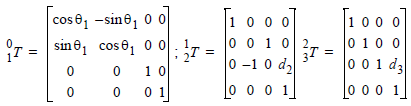
\includegraphics[width=9cm]{./bilder/denavitmatrix} \\
\end{minipage} \\
\clearpage

\section{Kinematik}
\subsection{Jacobi Matrix}

Die Jacobi-Matrix eines Roboterarms beschreibt die Abbildung von
Gelenkgeschwindigkeiten auf die Lineargeschwindigkeit des TCP
und die zeitlichen Änderungen der Orientierung des End-Effektors
bezogen auf ein Referenzkoordinatensystemk z.B. auf das
Basiskoordinatensystem O auf. \\
In der Positionsbeschreibung werden alle Parameter die einen Einfluss 
auf den Greifer haben aufgestellt und dann für die Jakobi-Matrix nach diesen Partiell abgeleitet.

\subsubsection{Vorwärtskinematik}
\begin{tabular}{lll}
    \textbf{Geg}&Gelenkkoordinaten und Geschwindigkeiten&$q,\; \dot{q}$\\
    &Vektor der Gelenkkoordinaten&$ q = \left[ q_1\; q_2 \;  \cdots \;  q_n\right]^T$\\
    &Vektor der Gelenkgeschwindigkeit&$ \dot{q} = \left[\dot{q}_1\; \dot{q}_2\; \cdots\;  \dot{q}_n \right]^T$\\
    \textbf{Ges}&Geschwindigkeit des Endeffektors:&$\dot{X}$\\
    &Vektor&$\dot{X} = [\dot{x}\; \dot{y}\; \dot{z}\;
    \dot{\gamma}\; \dot{\beta}\; \dot{\alpha}]^{T}$\\
\end{tabular}

\textbf{Lösung}: Jacobi-Matrix $ \Longrightarrow \dot{X}=J(q)\cdot \dot{q}$ \\ \\
\begin{minipage}{6cm}
\textbf{Jacobi-Matrix:} \\
$ \dot{X} = 
\underbrace{
\begin{bmatrix} 
\frac{\partial f_1}{\partial q_1} & \frac{\partial f_1}{\partial q_2} & \cdots & \frac{\partial f_1}{\partial q_{n}} \\
\frac{\partial f_2}{\partial q_1} & \frac{\partial f_2}{\partial q_2} & \cdots & \frac{\partial f_2}{\partial q_{n}} \\ 
\vdots & \vdots \\
\frac{\partial f_m}{\partial q_1} & \frac{\partial f_m}{\partial q_2} & \cdots & \frac{\partial f_m}{\partial q_{n}} \\
\end{bmatrix} }_{\text{Jacobi Matrix J(q)}}
\begin{bmatrix} 
\dot{q_1}\\
\dot{q_2}\\
\vdots \\
\dot{q_n}\\
\end{bmatrix} 
$
\end{minipage}
\begin{minipage}{12cm}
\begin{minipage}[b]{6cm}
    \textbf{Analytische Jacobi-Matrix:}\newline
    \[ \dot{y}=\begin{pmatrix}
    \dot{p}\\
    \omega
    \end{pmatrix}=
    \begin{bmatrix}
    J_p(\theta)\\
    J_\omega(\theta)
    \end{bmatrix} 
    \cdot \dot{\theta}\]     
\end{minipage}
\begin{minipage}{5cm}
\begin{tabular}{ll}
    $ J_p(\theta)$& translatorische J-Submatrix\\
    $ J_\omega(\theta)$& rotatorische J-Submatrix \\
    $ \dot{p}$& Endeffektor-geschwindigkeit\\
    $  \omega$& Endeffektor-winkelgeschwindigkeit\\
\end{tabular}
\end{minipage}

Für die Jacobi Matrizen
empfehlen sich
Kurzschreibweisen:\newline
$ c_{12}=cos(\theta_{1} + \theta_{2}) $ \qquad
$ s_{12}=sin(\theta_{1} + \theta_{2}) $

\end{minipage}\\ \\


\begin{minipage}{12cm}
    \paragraph{Beispiel 1:} Zweiachsiger Planarroboter: \\	
    $
    \begin{bmatrix} 
    p_x \\
    p_y \\                             
    \end{bmatrix}
    =
    \begin{bmatrix} 
    l_1\cdot cos(\theta_1) + l_2 \cdot cos(\theta_1 + \theta_2)\\
    l_1\cdot sin(\theta_1) + l_2 \cdot sin(\theta_1 + \theta_2)\\                     
    \end{bmatrix}
    =
    \begin{bmatrix} 
    f_1(\theta_1,\theta_2)\\
    f_2(\theta_1,\theta_2) \\                             
    \end{bmatrix}
    $ \\
    \vspace{-0.5cm}
    \begin{align*}
    J(q)&=
    \begin{bmatrix} 
    \frac{\partial f_1}{\partial \theta_1}  &   \frac{\partial f_1}{\partial \theta_2}\\
    \frac{\partial f_2}{\partial \theta_1} & \frac{\partial f_2}{\partial \theta_2}\\          
    \end{bmatrix}\hspace{-2cm}
    &=&
    \begin{bmatrix} 
    -l_1\cdot s_1 - l_2\cdot s_{12}& -l_2 \cdot s_{12} \\
    l_1\cdot c_1 + l_2 \cdot c_{12} & l_2 \cdot c_{12}\\                     
    \end{bmatrix}\\                    
    \dot{X}
    &=
    \begin{bmatrix} 
    \dot{p}_x \\
    \dot{p}_y \\                             
    \end{bmatrix}
    &=&
    J(q) \cdot         
    \begin{bmatrix} 
    \dot{\theta}_1 \\
    \dot{\theta}_2 \\                             
    \end{bmatrix}\\
    \end{align*}
    
    \vspace{-0.8cm}\textbf{\qquad Bemerkung: Orientierung wurde nicht berücksichtigt.}       
\end{minipage}        
\begin{minipage}{8cm}
    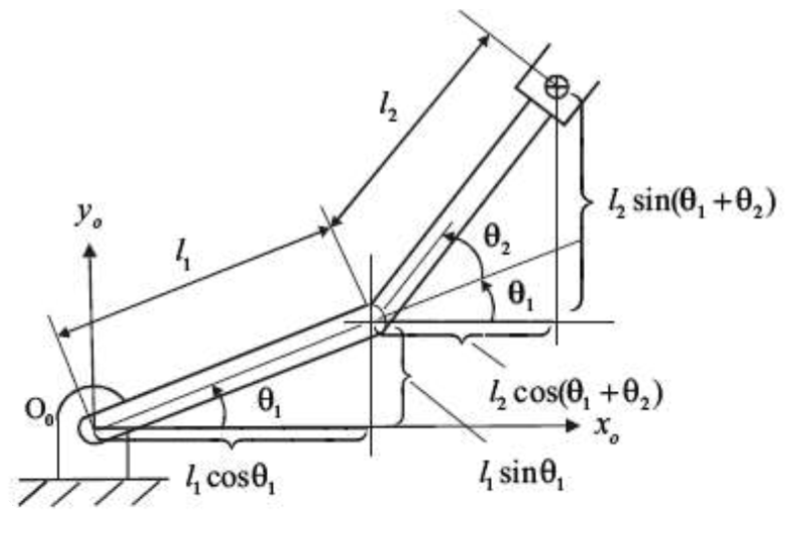
\includegraphics[width=7cm]{./bilder/jacobi-bsp1.png}
\end{minipage}

\begin{minipage}{14cm}
    \vspace{0.5cm}	
    \paragraph{Beispiel 2: }Dreiachsiger Planarroboter: \\
    $
    \begin{bmatrix} 
    x_E \\
    Y_E \\                             
    \end{bmatrix}
    =
    \begin{bmatrix} 
    l_1\cdot cos(\theta_1) + l_2 \cdot cos(\theta_1 + \theta_2) + l_3\cdot cos(\theta_1 + \theta_2 + \theta_3)\\
    l_1\cdot sin(\theta_1) + l_2 \cdot sin(\theta_1 + \theta_2) + l_3\cdot sin(\theta_1 + \theta_2 + \theta_3)\\                     
    \end{bmatrix} \newline
    \null \qquad \gamma = \theta_1 + \theta_2 + \theta_3
    $ \\ \\
    $ J = 
    \begin{bmatrix} 
    \frac{\partial{x_{e}}}{\partial{\theta_{1}}} & 
    \frac{\partial{x_{e}}}{\partial{d_{2}}} & 
    \frac{\partial{x_{e}}}{\partial{\theta_{3}}} \\
    \frac{\partial{y_{e}}}{\partial{\theta_{1}}} & 
    \frac{\partial{y_{e}}}{\partial{d_{2}}} & 
    \frac{\partial{y_{e}}}{\partial{\theta_{3}}} \\
    \frac{\partial{\Phi_{e}}}{\partial{\theta_{1}}} & 
    \frac{\partial{\Phi_{e}}}{\partial{d_{2}}} & 
    \frac{\partial{\Phi_{e}}}{\partial{\theta_{3}}} \\ 
    \end{bmatrix}
    =
    \begin{bmatrix} 
    -l_1 \cdot s_1 -l_2 \cdot s_{12} -l_3\cdot s_{123} & -l_2\cdot s_{12} -l_3\cdot s_{123} & -l_3\cdot s_{123}\\
    l_1\cdot c_1 +l_2\cdot c_{12} +l_3\cdot c_{123} & l_2\cdot c_{12} + l_3\cdot c_{123} & l_3\cdot c_{123}\\
    1 & 1 & 1\\
    \end{bmatrix}
    \\
    \dot{X}
    =
    \begin{bmatrix} 
    \dot{p}_x \\
    \dot{p}_y \\                             
    \end{bmatrix}
    =
    J(q) \cdot         
    \begin{bmatrix} 
    \dot{\theta}_1 \\
    \dot{\theta}_2 \\                             
    \end{bmatrix}$
\end{minipage}
\begin{minipage}{7cm}
    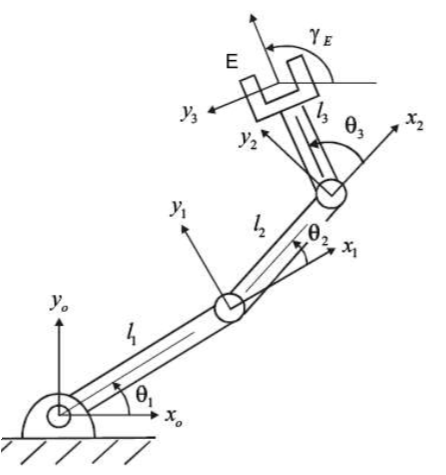
\includegraphics[width=5cm]{./bilder/jacobi-bsp2.png}
\end{minipage}

\clearpage
\subsubsection{Rückwertskinematik}
\begin{tabular}{lll}
    \textbf{Geg}&Geschwindigkeiten des Endeffektors&$\dot{X}$\\
    \textbf{Ges}&Geschwindigkeit der Gelenke&$\dot{q}$\\
\end{tabular}\newline
\textbf{Lösung}: inverse Jacobi-Matrix $ \Longrightarrow \dot{q}=J(q)^{-1}\cdot \dot{x}$ \\
\null\qquad\qquad Nur möglich, wenn J invertierbar ist. (Det $\neq$ 0)

%\paragraph{Beispiel 3: }zweiachsiger Planarroboter: \\
%$J^{-1}=\frac{1}{det(J)}\cdot
%\begin{bmatrix}
%    l_2\cdot c_{12} & l_2 \cdot s_{12}\\
%    -l_1\cdot c_1 - l_2\cdot c_{12} & -l1\cdot s_1 -l_2\cdot s_{12}
%\end{bmatrix}
%$
\subsubsection{Singularität}
Die Jacobi-Matrix kann in singulären Stellungen
nicht invertiert werden (d.h. die Determinante von J ist 0) und der Roboter
kann in bestimmten Richtungen keine Bewegungen
vornehmen. \\
In der Nähe von Singularitäten könnnen die Achsengeschwindigkeiten extrem ansteigen.
%Mehr: Skript-Kinematik (S.11 ff) \& UB5 Bahnplanung (Aufg. 2))
\begin{multicols}{2}
\paragraph{Beispiel 3.1} Singularitätsbestimmung eines zweiachsigen Planarroboters\newline
\null\hspace{0.5cm}\begin{tabular}{ll}
    \textbf{Gegeben:}& Jacobi-Matrix\\
    \textbf{Gesucht:}& Singularität\\
    \textbf{Vorgehen:} & det(J)= 0 setzen\\
\end{tabular}
\paragraph{Beispiel 3.2} Geschwindigeit in singulärer Stellung\newline
\null\hspace{0.5cm}\begin{tabular}{ll}
    \textbf{Gegeben:}& Jacobi-Matrix\\
    \textbf{Gesucht:}& Geschwindigeit\\
    \textbf{Formel:} & $ \dot{\theta}= J^{-1}\cdot \dot{x}$\\
    \textbf{Vorgehen:} & det(J) $\rightarrow$ 0 \\
\end{tabular}
\end{multicols}
\subsection{Roboterstatik}
Momente, welche an den Achsgelenken wirken:\newline
$\tau_{n}={}^0J^T_n \cdot {}^0F_n$  \\
Externe Momente / Kräfte, welche am n-ten Glied wirken:\newline
${}^0F_n = \begin{bmatrix} {}^0F_{x,n} & {}^0F_{y,n} & {}^0F_{z,n} & {}^0M_{x,n}
& {}^0M_{y,n} & {}^0M_{z,n}
\end{bmatrix}^{T} $ \newline
\paragraph{Beispiel 4} Kräfte eines zweichasigen Planarroboter\newline
Der Roboter soll mit dem globalen Kraftvektor ${}^0F$ gegen einen foxen Körper drücken.\newline
\null\hspace{0.5cm}\begin{tabular}{ll}
    \textbf{Gegeben:}& Jacobi-Matrix\\
    \textbf{Gesucht:}& erforderliches Antriebsmoment $\tau_1$ und $\tau_2$\\
    \textbf{Vorgehen:} & $\tau_{n}={}^0J^T_n \cdot {}^0F_n$  \\
\end{tabular}$\null \qquad\qquad
\begin{bmatrix}
\tau_{1} \\ \tau_{2} \\ \tau_{3}
\end{bmatrix}          
=  J \cdot
\begin{bmatrix}
F_{x} \\ F_{y} \\ F_{z}
\end{bmatrix}
$
\clearpage


\clearpage
\section{Dynamik \robo{124}{6}}
\vspace{-0.5cm}
\begin{center} 
     \[ \texttt{Gelenkekräfte/Momente } Q
     \mathrel{\mathop{\rightleftarrows}^{\mathrm{Direkte Dynamik}}_{\mathrm{Inverse Dynamik}}}
      \texttt{Bewegung des Arbeitsgliedes } \ddot{q},\; \dot{q},\; q\]   
\end{center}

\begin{minipage}{\linewidth}
    \small 
    \begin{tabular}{p{3cm} p{2.7cm} p{3.2cm} p{3.2cm}}
        \hline
        \textbf{physikalische Grösse} & \textbf{generalisierten Beschreibung} &
        \textbf{Bezeichnung bei einem Schubgelenk}&
        \textbf{Bezeichnung bei einem Drehgelenk}\\ \hline
        generalisierte Koordinate & q &\textit{d} in [m]& $\theta$ in [rad]\\
        Masse, Trägheitsmoment & M & \textit{m} in [kg] & $J_L$ in [$kgm^2$]\\
        antreibende Kraft bzw. Moment & $\tau$ & \textit{F} in [N]& $M_{Gel}$ in [Nm]\\
        Verschiedene Kräfte/ Drehmomente & $b(q,\dot{q})$ & $\hat{F}_D \cdot \dot{d}+ m \cdot g \cdot \sin\beta $& $F_D \cdot \dot{\theta} + m \cdot g \cdot l_s \cdot \cos \theta$\\ 
        \hline  
    \end{tabular}
    \hspace{0.5cm}\begin{minipage}{4cm}
        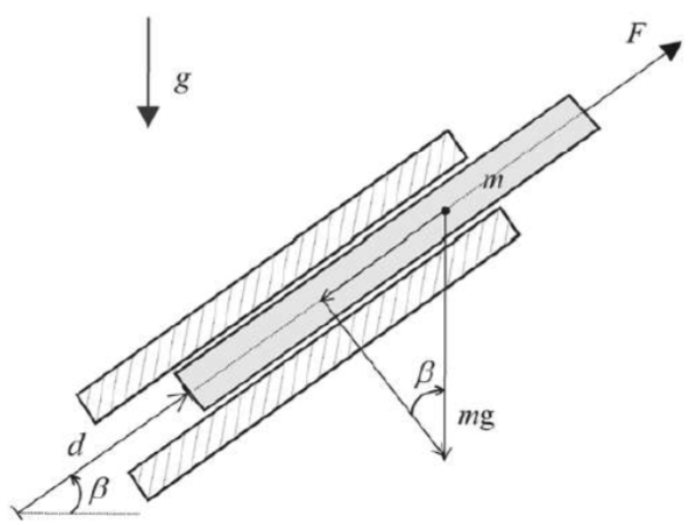
\includegraphics[width=0.9\linewidth]{./bilder/DynSchubgelenk}\newline
        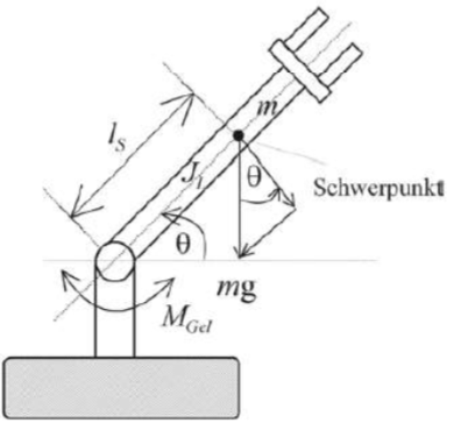
\includegraphics[width=0.8\linewidth]{./bilder/DynDrehgelenk}
    \end{minipage}
\end{minipage}
\begin{tabular}{p{4cm}p{6cm}p{7.5cm}}
    \textbf{Dynamische Gleichung} \newline Roboter mit n Achsen&
    $Q = M(q)\cdot \ddot{q} + V(q,\dot{q})+ G(q)  $ \newline
    $\tau \;= M(q) \cdot \ddot{q} + b(q,\dot{q}) \;+ z $&
    \multirow{2}{7.5cm}{\small{ 
        Q: verallgemeinerte Kräfte (n\texttimes 1)\newline
        M: konfigurationsabhängige Massenmatrix (n\texttimes n)\newline
        V: Vektor nichtlinearer Term, der durch die Zentripetal- und die Coriolis-Beschleunigung entsteht (n\texttimes 1)\newline
        G: Vektor, der die Gravitationsterme enthält (n \texttimes 1)
    }}\\
    \textbf{1 DOF Manipulator}& $ \tau = ml^2\cdot \ddot{q}+mgl \cdot \cos(q) + c \cdot sgn(\dot{q} + v \cdot \dot{q}) $&\\
    \textbf{Bewegungsgelichung}\newline
    \robo{144}{6.2.6}&
    $\ddot{q}=M^{-1}(q)[\tau -b(q,\dot{q})]$&
    \\
\end{tabular}

\subsection{Dynamik nach Lagrange}
\begin{tabular}{p{4cm}p{6cm}p{7.5cm}}
    \hline
    \textbf{Kinematische Energie eins Robotergiled i}&
    \[ \hspace{-0.5cm} E_{Kin, \; i} = \frac{1}{2} \cdot v_{Si}^T \cdot m_i \cdot v_{Si}+ \frac{1}{2} \cdot\omega_i^T  \cdot{}^0l_i  \cdot\omega_i \]
    \[ \hspace{-0.5cm} {}^0\dot{x}_{Si}=\begin{bmatrix}
    V_{Si}\\
    \omega_i
    \end{bmatrix}= {}^0 J_i \cdot \dot{q} \qquad{}^0J_i = \begin{bmatrix}
    J_{Ti}\\
    J_{Ri}
    \end{bmatrix} \]
&
   \small{
    $v_{Si}$: Geschwindigkeit des Schwerpunktes S vom Roboterglied i \newline
    $m_i$: Masse von Roboterglied i\newline
    ${}^0l_i$: Trägheitsmatrix von Roboterglied i (bezogen auf Schwerpunkt von i und ausgedrückt im Basiskordinatensystem \{0\}) \newline
    ${}^0J_i$: auf Roboterglied i bezogenen Jacobi-Matrix
    }\\\hline

    \textbf{Kinematische Energie aller Roboterglieder n}&
        \[ \hspace{-0.5cm} E_{Kin} = \frac{1}{2}\sum_{i=1}^{n}( v_{Si}^T \cdot m_i \cdot v_{Si}+ \cdot\omega_i^T  \cdot{}^0l_i  \cdot\omega_i )\]&\\ \hline
\end{tabular}
%\clearpage

\begin{minipage}{0.5\linewidth}
    \textbf{Kinetische Energie}\\
    \[ E_{Kin}= \frac{1}{2} \cdot \dot{q}^T \cdot M\cdot \dot{q}  \]
    mit der Roboterträgheitsmatrix:\newline
    \[ M = \sum_{i=1}^{n} ( J_{Ti}^T \cdot m_i \cdot J_{Ti} + J_{Ri}^T \cdot {}^0l_i \cdot J_{Ri}) \]
    \[ \hspace{-0.3cm}E_{Kin}= \frac{1}{2} \cdot \dot{q}^T \cdot \left[ \sum_{i=1}^{n} ( J_{Ti}^T \cdot m_i \cdot J_{Ti} + J_{Ri}^T \cdot {}^0l_i \cdot J_{Ri}) \right]\cdot \dot{q} \]
\end{minipage}
\begin{minipage}{0.5\linewidth}
    \textbf{Potentielle Energie}\\
    \[ E_{Pot}=-\sum_{i=1}^{n} m_i \cdot g^T \cdot r_{Si} \]
    g: Vektor der Gravitationsbeschleunigung\newline
    $r_{Si}$: Vektor der von der Referenzposition auf den Massenschwerpunkt von Glied i weist
    \vspace{1.8cm}
\end{minipage}
\clearpage

\begin{minipage}{\linewidth}
    \begin{minipage}{0.5\linewidth}
        \subsubsection{Lagrange Gleichung}
        \vspace{-0.5cm}
        \[ L=E_{Kin}-E_{Pot} \]
        \[ L= \frac{1}{2}\cdot \dot{q}^T \cdot M \cdot \dot{q} -(- \sum_{i=1}^{n}(m_i \cdot g^T \cdot r_{Si})) \]
    \end{minipage}
    \begin{minipage}{0.5\linewidth}
        \[ Q_j = \frac{\diff}{\diff t} \left(\frac{\partial L}{\partial \dot{q}_j} - \frac{\partial L}{\partial q_j}\right) \quad \texttt{mit}\quad j=1,2,\dots, n\]
        $Q_j$= verallgemeinerte Kräfte\newline
        $q_j$= verallgemeinerte Koordinaten
    \end{minipage}
\end{minipage}


\begin{minipage}{0.75\linewidth}
    \subsubsection{Bewegungsgleichung \robo{144}{6.2.6}}
    \vspace{-0.5cm}
    \[\hspace{-0.5cm}\begin{pmatrix}
        \tau_1\\
        \tau_2
    \end{pmatrix}=
    \underbrace{
    \begin{bmatrix}
    b_{11}&b_{12}\\
    b_{21}&b_{22}
    \end{bmatrix}}_{\texttt{Beschleunigung}}
    \begin{pmatrix}
    \ddot{\theta}_1\\
    \ddot{\theta}_2
    \end{pmatrix}+
    \underbrace{
    \begin{bmatrix}
    0 &h_{1,22}\\
    h_{2,11}&0\\
    \end{bmatrix}}_{\texttt{Zentrifugal}}
    \begin{pmatrix}
    \dot{\theta}_1^2\\
    \dot{\theta}_2^2
    \end{pmatrix}+
    \underbrace{
    \begin{bmatrix}
    h_{1,12} & 0\\
    0&0\\
    \end{bmatrix}}_{\texttt{Coriolis}}
    \begin{pmatrix}
    \dot{\theta}_1 \dot{\theta}_2\\
    \dot{\theta}_2 \dot{\theta}_1
    \end{pmatrix} +
    \underbrace{
    \begin{pmatrix}
    g_1\\
    g_2\\
    \end{pmatrix}}_{\texttt{Gravitation}}
    \]
\end{minipage}
\begin{minipage}{0.25\linewidth}
    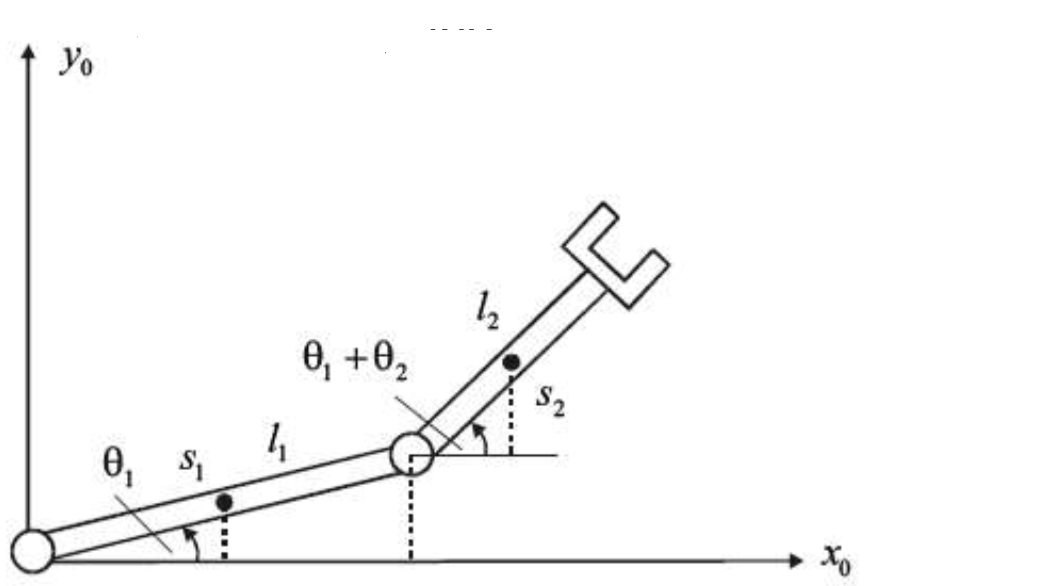
\includegraphics[width=\linewidth]{./bilder/PlanarRoboterBewegungsgleichung}
\end{minipage}

\begin{minipage}{0.7\linewidth}
    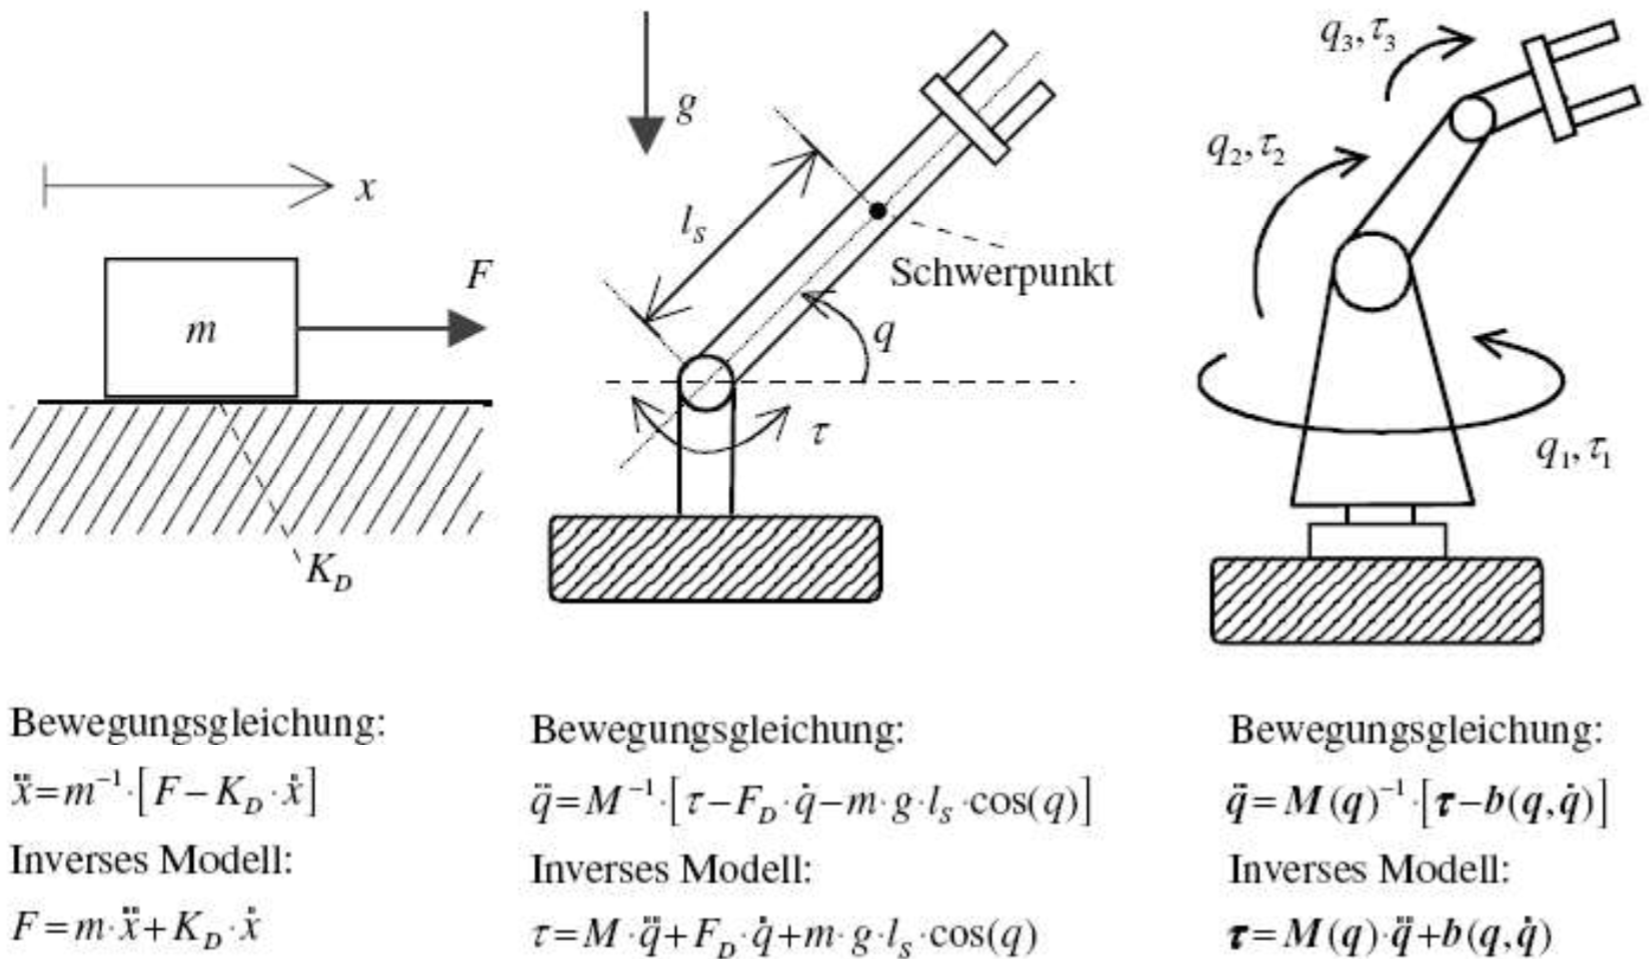
\includegraphics[width=\linewidth]{./bilder/DynMod}
\end{minipage}\\
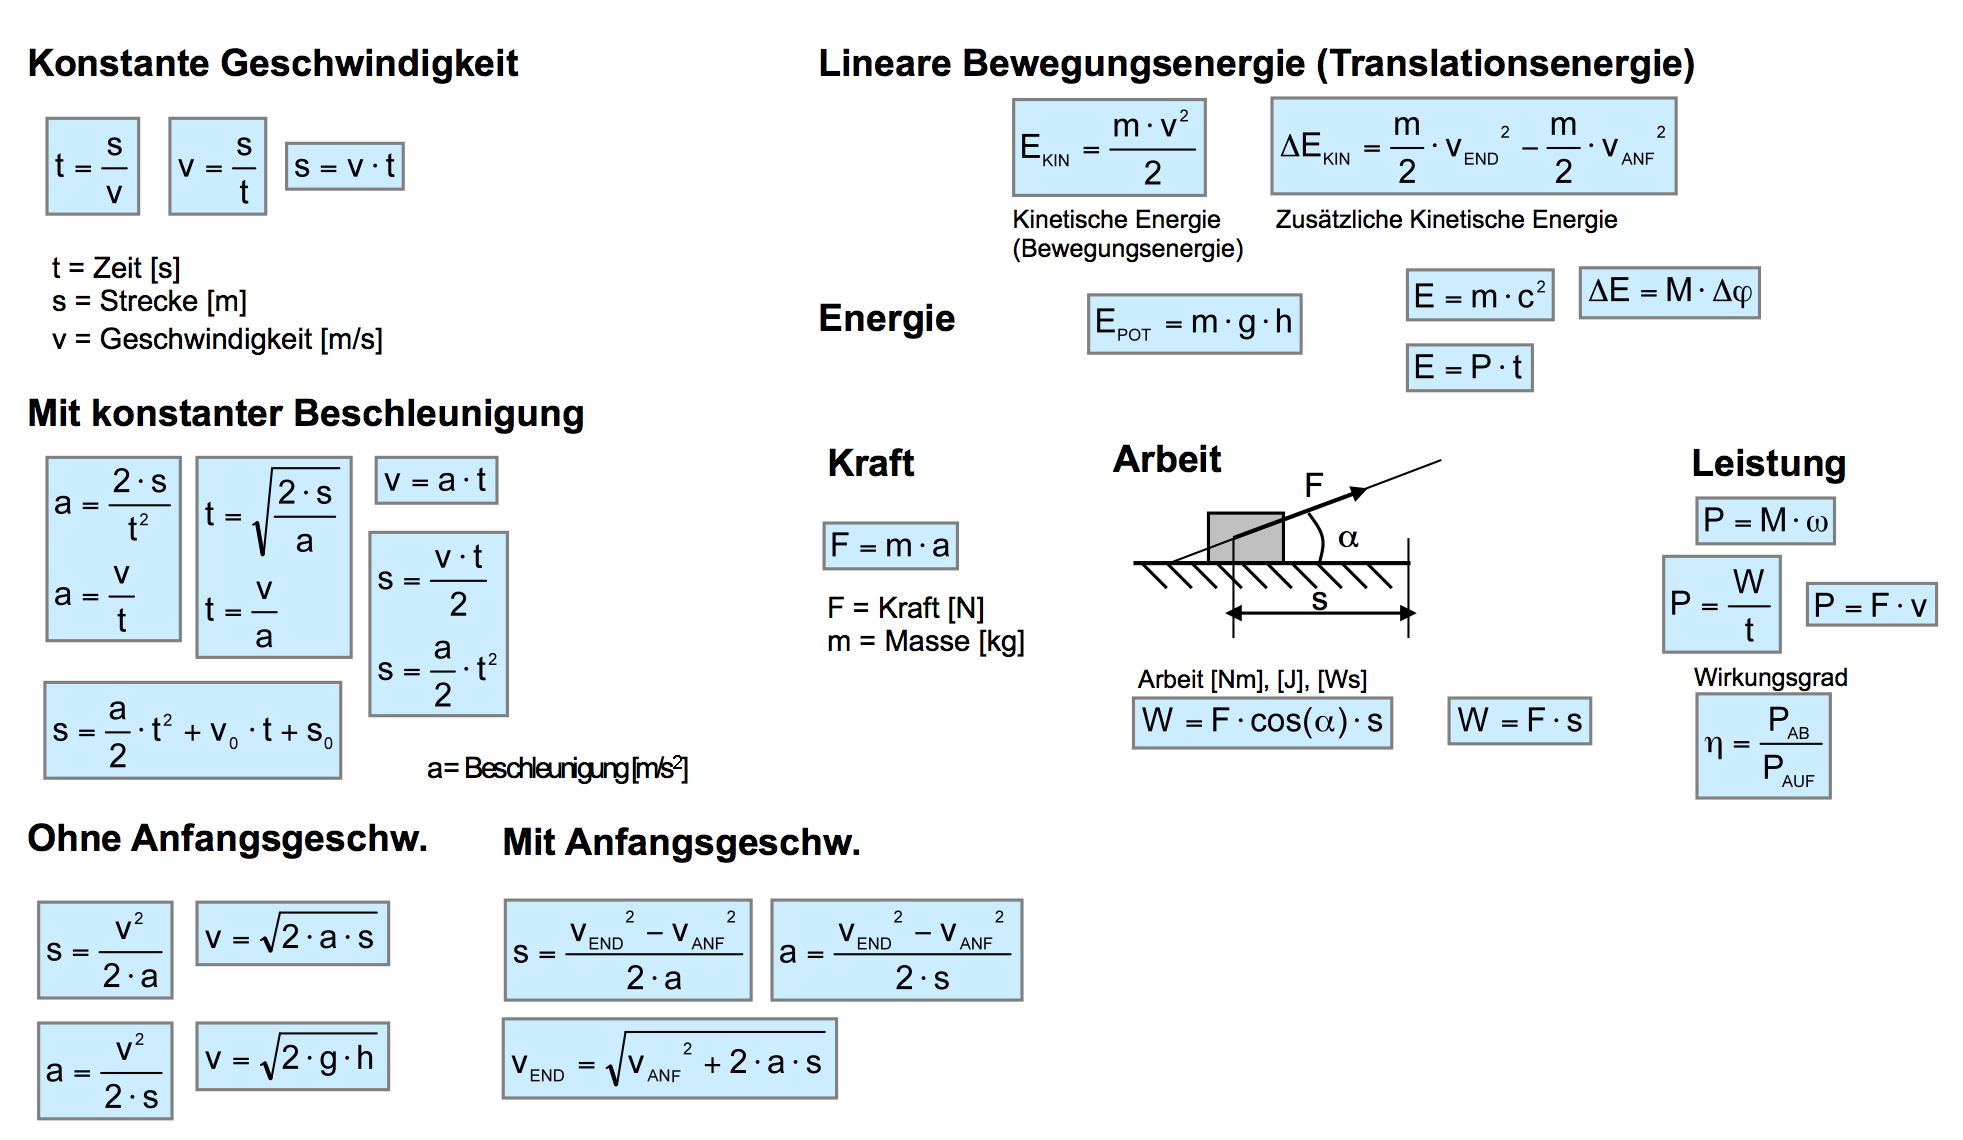
\includegraphics[width=17cm]{./bilder/kinematik}



\clearpage
\section{Bahnplanung}
\subsection{Bewegungsarten}
\begin{minipage}{0.5\linewidth}
    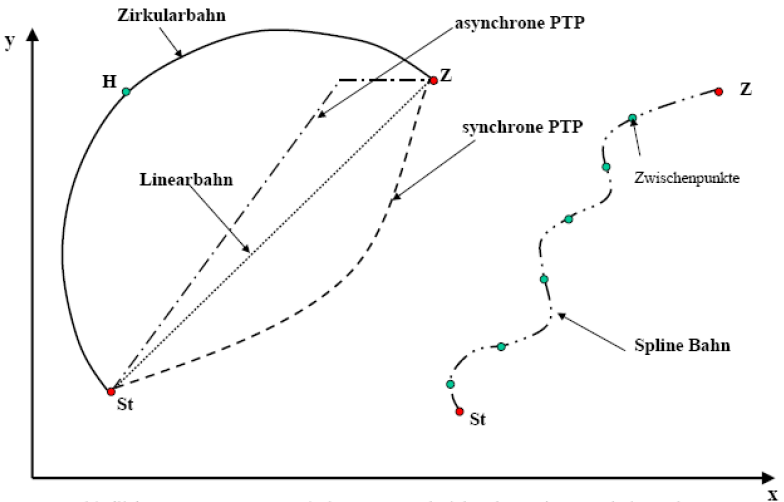
\includegraphics[width=\linewidth]{./bilder/bewegungsarten.png}
\end{minipage}
\begin{minipage}{0.5\linewidth}
    \includegraphics[width=\linewidth]{./bilder/Bewegunggreifer.png}
\end{minipage}

\begin{minipage}{0.5\linewidth}
    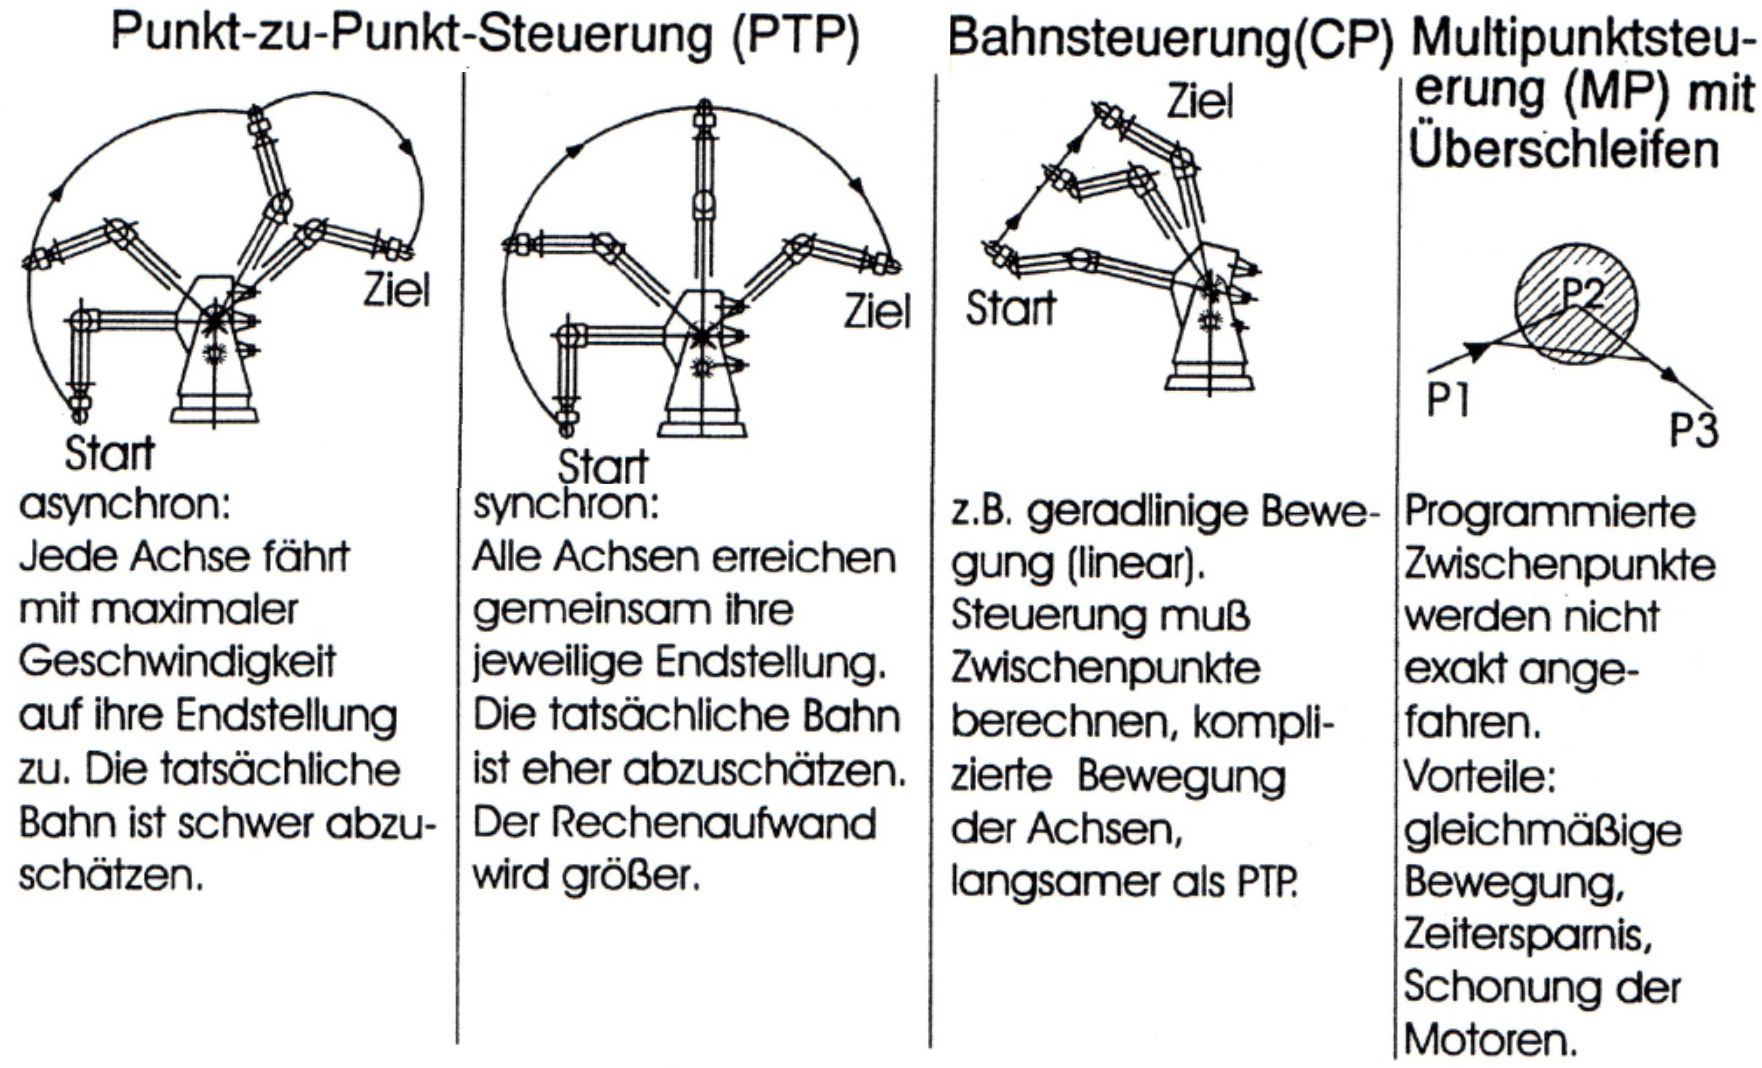
\includegraphics[width=\linewidth]{./bilder/bewegungsarten2.png}
\end{minipage}
\begin{minipage}{0.5\linewidth}
    \begin{itemize}
        \item  \textbf{asynchronen PTP}
        \begin{itemize}
            \item  Jede Achse verfährt vollständig unabhängig von anderen Achsen.
        \end{itemize}
        \item  \textbf{synchronen PTP}
        \begin{itemize}
            \item  Wird durch die Achse mit der grössten Bahndauer bestimmt.
            \item Die Geschwindigkeit der anderen Achsen wird reduziert,so dass alle gleichzeitig ihren Endpunkt erreichen.
        \end{itemize}
        \item  \textbf{vollsynchronen PTP}
        \begin{itemize}
            \item  Nicht nur die Bahnzeiten für die Gelenke synchronisiert.
            \item Auch Beschleunigungs und Brmezeiten synchron.
        \end{itemize}
    \end{itemize}
\end{minipage}
\vspace{-1cm}
\subsubsection{Singularität}
\begin{minipage}{0.5\linewidth}
    \textbf{Singuläre Konfiguration}
    \begin{itemize}
        \item Mehrere Achsen liegen in einer Linie
        \item Die Drehung einer Achse kann durch Gegendrehung einer anderen Achse kompensiert werden.
        \item Ein Freiheitsgrad geht verloren, da für eine Drehachse zwei Gelenke verwendet werden.
    \end{itemize}
\end{minipage}
\begin{minipage}{0.5\linewidth}
    \textbf{Grenzsingularität}\newline
    \begin{itemize}
        \item Der Roboter ist ganz ausgestreckt oder an einer Position am Rande seines Arbeitsraum
        \begin{itemize}
            \item Es gibt Richtungen in die er sich nicht mehr bewegen kann
        \end{itemize}
    \end{itemize}
\end{minipage}

\subsection{Bahnüberschleifen}
Vorteile:
\begin{itemize}
    \item[+] Zeitgewinn
    \item[+] Vermeidung von ruckartigen Bewegungen
    \item[+] Hindernisumfahrung durch Definition von Zwischenpunkten 
\end{itemize}

\begin{minipage}{0.345\linewidth}
    \textbf{PTP}\newline
    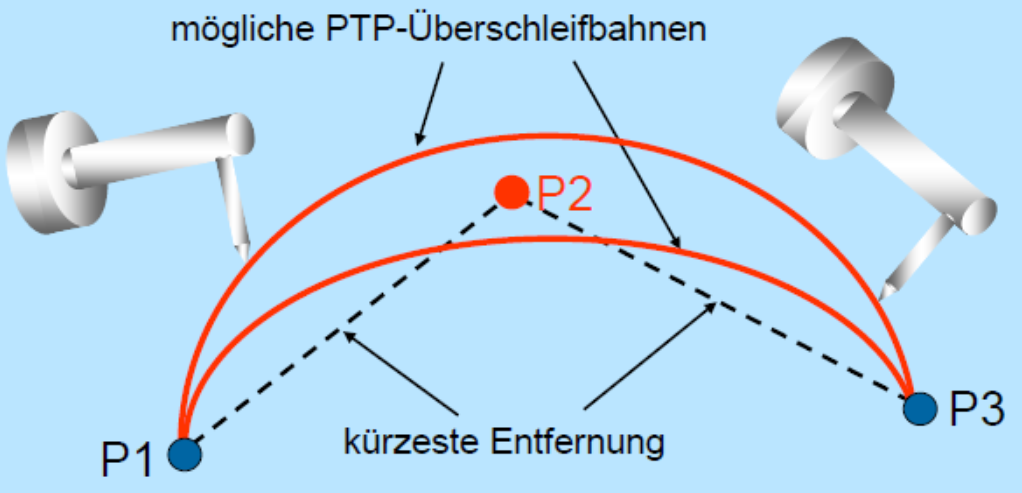
\includegraphics[width=\linewidth]{./bilder/UeberschleifenPTP.png}
\end{minipage}
\begin{minipage}{0.32\linewidth}
    \textbf{Linear}\newline
    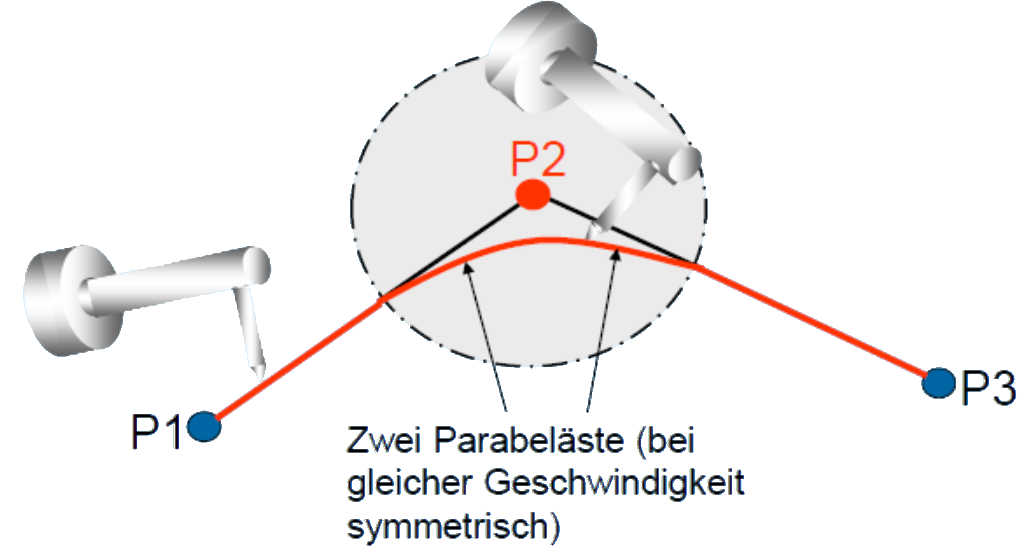
\includegraphics[width=\linewidth]{./bilder/UeberschleifenLin.png}
\end{minipage}
\begin{minipage}{0.32\linewidth}
    \textbf{Zirkular}\newline
    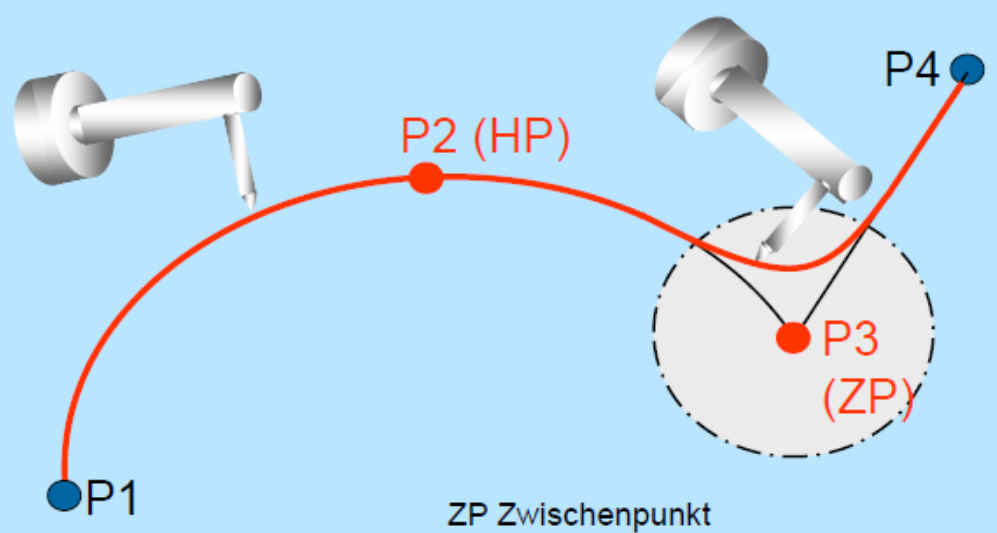
\includegraphics[width=\linewidth]{./bilder/UeberschleifenCirc.png}
\end{minipage}

\subsection{Bahnerzeugungn in Gelenkkoordinaten}
\begin{multicols}{2}
    \begin{itemize}
        \item[+] Minimale Bewegung bei jedem Gelenk.
        \item[+] Max. Geschwindigkeit und max. Momente bekannt.
    \end{itemize}

    \begin{itemize}
        \item[-] Bahngeometrie in kart. Raum unbekannt.
        \item[-] Kollisionsvermeidung schwierig.
    \end{itemize}
\end{multicols}

\subsubsection{Kubisches Polynome}
\begin{tabular}{ll}
\multicolumn{2}{l}{\textbf{Bedingungen}}\\
$ \theta(0)=\theta_0 $& $ \theta(t_f) = \theta_f$\\ 
$ \dot{\theta}(0)=0 $& $ \dot{\theta}(t_f) = 0$\\
\multicolumn{2}{l}{\textbf{Gleichung}}\\
\multicolumn{2}{l}{$ \theta(t)=a_0 + a_1t + a_2t^2+a_3t^3$}\\
\multicolumn{2}{l}{\textbf{Koeffizienten}}\\
$a_0= \theta_0$&$a_1=0 $\\
$a_2 = \frac{3}{t_f^2}(\theta_f - \theta_0) $&$a_3=-\frac{2}{t_f^3}(\theta_f-\theta_0) $\\
\end{tabular}
\paragraph{Bsp.}
Ein Roboter mit einer Rotationsachse ($\theta$) soll sich von $\theta$= -5\textdegree bis zu $\theta$= 80\textdegree in 4 Sekunden bewegen.\newline
Gesucht: Koeff des kubischen Polynoms, max Geschwindigkeit und max Beschleunigung der Achsen.
Stellen sie die Position Grafisch dar.

\begin{tabular}{ll}
    Kubisches Polynom & $\theta(t)=a_0 + a_1t + a_2t^2+a_3t^3$\\
                        & $a_0 = -5$\textdegree$,\; a_1=0,\; a_2=15.93,\; a_3=-2.656 $\\
    Geschwindigkeit     & $\dot{\theta}=a_1+2a_2\cdot t+3a_3 \cdot t^2 $\\
                        & $ \qquad 31.86 \cdot t - 7.968 \cdot t^2$\\
    Beschleunigung      & $ \ddot{\theta}=2a_2 + 6a_3 \cdot t$\\
                        & $ \qquad 31.86 - 15.936 \cdot t$\\
    $\rightarrow \ddot{\theta}=0 $ & t = $\frac{31.86}{15.936}=2s$\\
    max. Geschw.        & $ \dot{\theta}_{max}= 31.86\cdot 2s - 7.968\cdot 4s = 31.848$\textdegree$ /s$\\
    max. Besch.         &$ \ddot{\theta}_{max} \rightarrow t=0 $ \\  
                        &$ \ddot{\theta}_{max} \rightarrow t=t_f $ \\              
\end{tabular}


\subsubsection{Rampenprofil}
\begin{minipage}{0.5\linewidth}
    {\small 
    $\ddot{\theta}$ gegeben\newline
    \begin{align*}
        \ddot{\theta}\cdot t_b &= \frac{\theta_h-\theta_b}{t_h - t_b}\\
        \theta_b &=\theta_0 + \frac{1}{2}\ddot{\theta}\cdot t_b^2\\
        t_b &= \frac{t}{2}- \frac{\sqrt{t^2\cdot \ddot{\theta}^2-4\ddot{\theta}\cdot(\theta_f)- \theta_0}}{2\ddot{\theta}}\\
        t_h &= \frac{1}{2}t_f\\
        \theta_h &=\frac{1}{2}(\theta_f -\theta_0)
    \end{align*}
    \begin{tabular}{ll}
        $t_b$ & Länge des Übergangs\\
        $t_f$ & Dauer der Bewegung\\
        $t_h$ & \\
        $\theta_b$& Ende des Übergangs\\
        $\theta_h$& \\
        $\ddot{\theta}$& Beschleunigung während des Übergangs\\
    \end{tabular}}
\end{minipage}
\begin{minipage}{0.5\linewidth}
    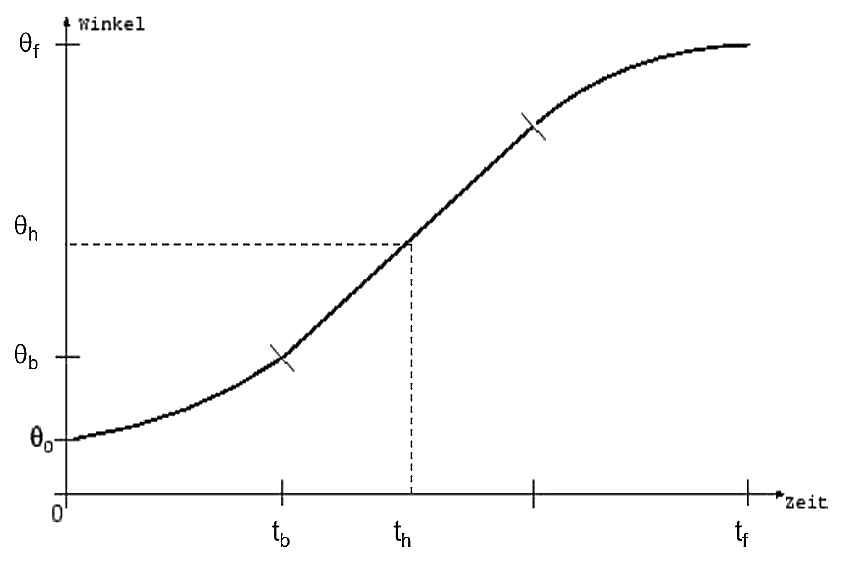
\includegraphics[width=\linewidth]{./bilder/RampenprofilInterpol}
\end{minipage}
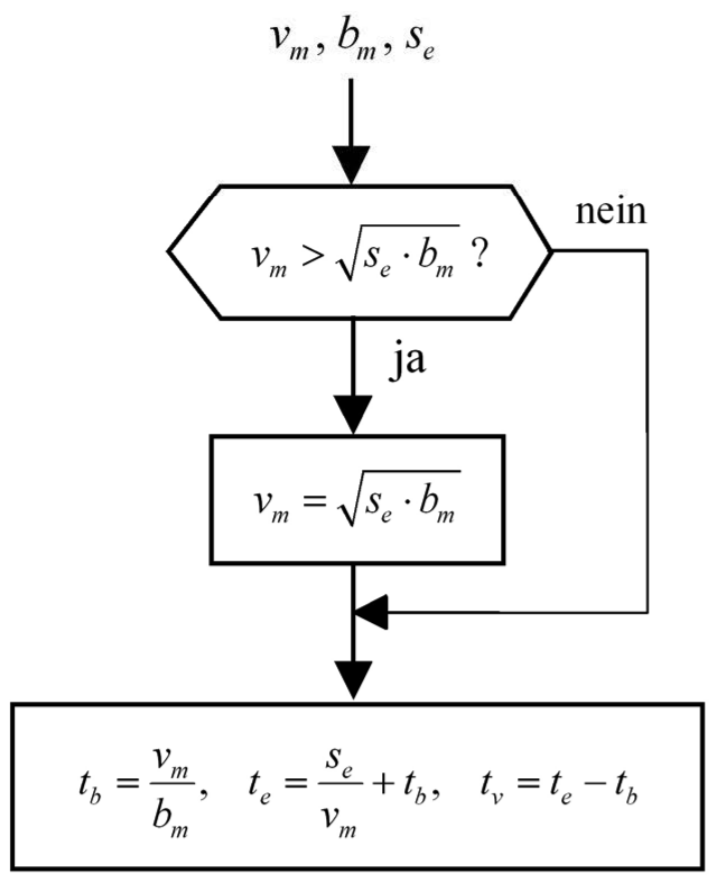
\includegraphics[width=0.3\linewidth]{./bilder/RampenVorgehn}

\subsection{Bahnerzeugungn in karteschien Koordinaten}
\begin{multicols}{2}
    \begin{itemize}
        \item[+] Bahn genau definiert
    \end{itemize}
    
    \begin{itemize}
        \item[-] Berechnung der inv. Koordtrans für jeden Punkt notwendig.
        \item[-] Geometrische Probleme
        \begin{itemize}
            \item Unerreichbare Zwischenpunkte
            \item Hohe v in der näche von Singularitäten
            \item Start/Ziel gehören zu verschiedenen Zweige der kin. Lösung
        \end{itemize}
        \item[-] Schwierig, die Motorenbegrenzung zu berücksichtigen.
    \end{itemize}
\end{multicols}
\clearpage
\section{Roboterregelung}
\clearpage
\section{Kollaborative Robotik}
Menschen und Roboter teilen sich den selben Arbeitsraum.
Die Wiederholgenauigkeit und Ausdauern von Robotern sollen mit den individuellen Fähigkeiten von Menschen kombiniert werden.\newline
\begin{minipage}{0.49\linewidth}
\begin{itemize}
    \item Sicherheit
    \begin{itemize}
        \item Ohne Schutzeinrichtung
        \begin{itemize}
            \item weniger platz
            \item mobil
        \end{itemize}
        \item Kraft-Drehmomentsensorik
        \item Reduzierte Geschwindigkeit   
    \end{itemize}
    \item Eigenschaften
    \begin{itemize}
        \item[+] Platzsparend
        \item[+] bezahlbar
        \item[+] felxibel
        \item[+] Kraftempfindlichkeit
        \item[-] Langsam
    \end{itemize}
    \item Applikation
    \begin{itemize}
        \item Qualtitätskontrolle
        \item Montage (3te-Hand)
        \item Handling
    \end{itemize}
\end{itemize}
\end{minipage}
\begin{minipage}{0.5\linewidth}
    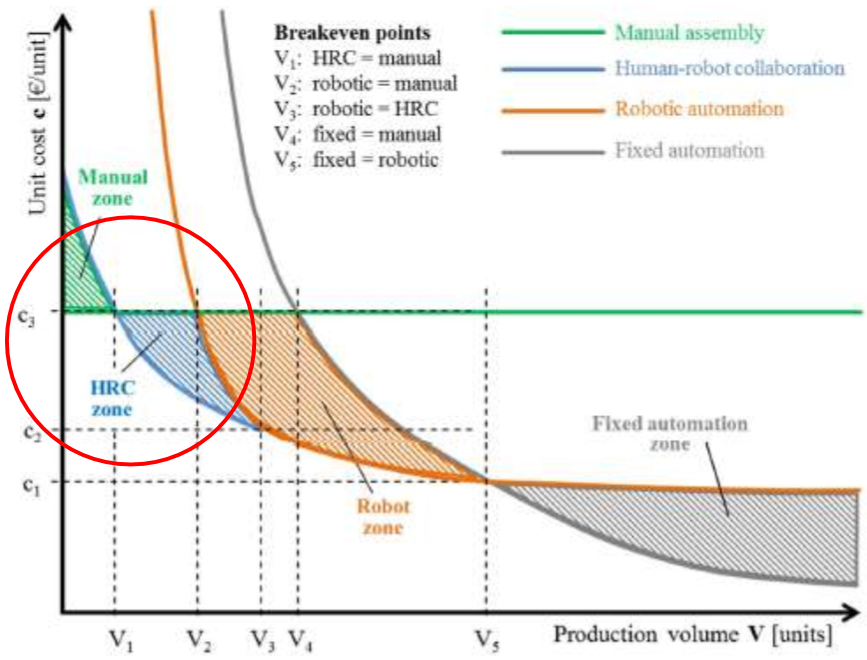
\includegraphics[width=\linewidth]{./bilder/wirtschaft}
\end{minipage}
\subsection{MRK-Schutzarten}
\begin{minipage}{\linewidth}
    \subsubsection{Sicherer Halt}
    \begin{minipage}{0.7\linewidth}
    \textbf{Methode 1}\newline
    \begin{tabular}{p{2.2cm} p{10cm}}
        \textbf{Prinzip}&
        Roboterbewegung wird angehalten bevor eine Person den Kollaborationsraum betritt
        \\
        \textbf{Betriebsweise}&
        Wenn die Sicherheitsüberwachung aktiv und die Roboterbewegungn angehalten ist,
        ist es dem Bedienpersonal erlaubt, den Kollaborationsraum zu betretten.
        Das Robotersystem startet erst wider nach dme Verlassen des Personals aus dem Kollaborationsbereich.
        \\
        \textbf{Anwendungs -bereich}&
        Be- und Entladen \newline
        Kontrollieren der Werkstücke
        \\
    \end{tabular}
    \end{minipage}
    \begin{minipage}{0.3\linewidth}
    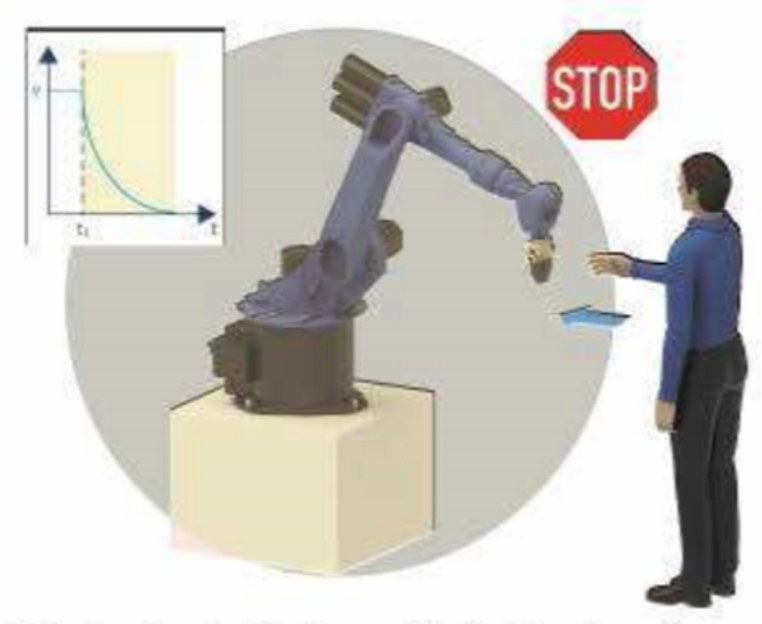
\includegraphics[width=\linewidth]{./bilder/SchutzMRKm1}
    \end{minipage}
\end{minipage}

\begin{minipage}{\linewidth}
    \subsubsection{Handführung}
    \begin{minipage}{0.7\linewidth}
    \textbf{Methode 2}\newline
    \begin{tabular}{p{2.2cm} p{10cm}}
        \textbf{Prinzip}&
        Roboterbewegung wird vom Mitarbeiter aktiv mit geeigneter Ausrüstung gesteuert.
        \\
        \textbf{Betriebsweise}&
        Bevor die Bedienperson den Kollaborationsraum betreten darf, führt das Robotersystem einen überwachten Halt aus.
        Die Aufgabe wird durch manuelle Betätigung der Führungseinrichtung, die sich am Endeffektor des Roboters oder dessen nähe befindet, ausgeführt.
        \\
        \textbf{Anwendungs- bereich}&
        Handgeführte Montagen, Lackieren\newline
        Roboter als Montage-Tool\newline
        Produktion mit kleiner Stückzahl
        \\
    \end{tabular}
    \end{minipage}
    \begin{minipage}{0.3\linewidth}
    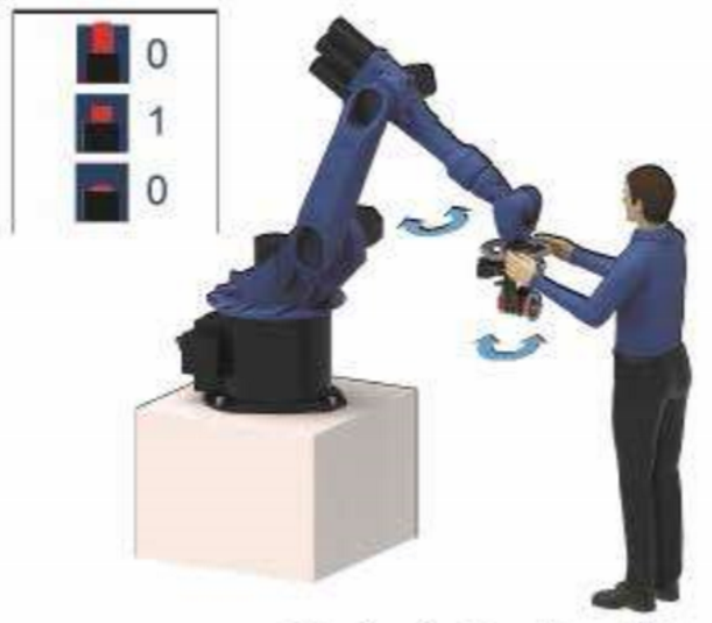
\includegraphics[width=\linewidth]{./bilder/SchutzMRKm2}
    \end{minipage}
\end{minipage}
\clearpage

\begin{minipage}{\linewidth}
    \subsubsection{Geschwindigkeits und Abstandsüberwachung}
    \begin{minipage}{0.7\linewidth}
    \textbf{Methode 3}\newline
    \begin{tabular}{p{2.2cm} p{10cm}}
        \textbf{Prinzip}&
        Kontakt zwischen Mitarbeiter und in Bewegung befindenden Roboter wird vom Roboter vermieden.
        \\
        \textbf{Betriebsweise}&
        Roboter und Bedienperson dürfen sich Gleichzeitig im Kollaborationsraum aufhalten. Es gilt ein Sicherheitsabstand. Wenn das Robotersystem seine Geschwindigkeit herabsetzt, verringert sich auch der Sicherheitsabstand.
        \\
        \textbf{Anwendungs- bereich}&
        Gemeinsame Montage und Handhabung
        \\
    \end{tabular}
    \end{minipage}
    \begin{minipage}{0.3\linewidth}
    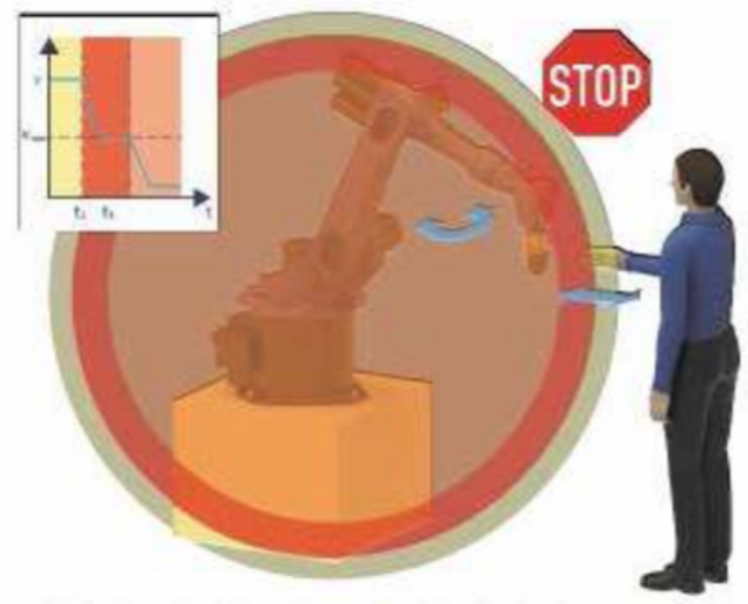
\includegraphics[width=\linewidth]{./bilder/SchutzMRKm3}
    \end{minipage}
\end{minipage}
\begin{minipage}{\linewidth}
    \subsubsection{Leistung und Kraftbegrenzung}
    \begin{minipage}{0.7\linewidth}
    \textbf{Methode 4}\newline
    \begin{tabular}{p{2.2cm} p{10cm}}
        \textbf{Prinzip}&
        Kontaktkräfte zwischen Mitarbeiter unf Roboter(inkl. Bauteil) werden technisch auf ein ungefährliches Mass begrenzt.
        \\
        \textbf{Betriebsweise}&
        Physischer Kontakt zwischen Robotersystem kann auftreten. Jedoch ist die maximale Kraft unterhalb der Belastungsgrenze welche bei der Risikobeurteilung bestimmt wurde.
        \\
        \textbf{Anwendungs- bereich}&
        Kontakt erforderlich(small part assembly)\newline
        Anwendungen, die häufig den Kontakt des Bedienpersonals erfordern
        \\
    \end{tabular}
    \end{minipage}
    \begin{minipage}{0.3\linewidth}
    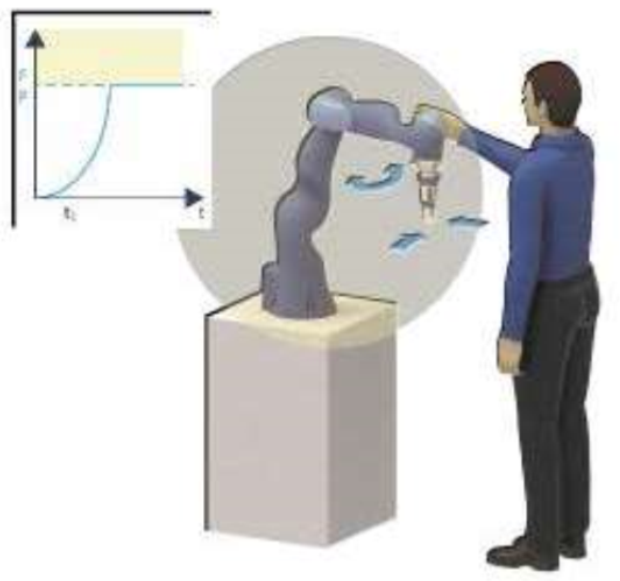
\includegraphics[width=\linewidth]{./bilder/SchutzMRKm4}
    \end{minipage}
\end{minipage}

\subsection{MRK-Arten}
\begin{minipage}[t]{\linewidth}
\begin{minipage}[t]{0.33\linewidth}
\textbf{Koexistenz}\hfill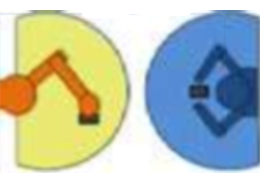
\includegraphics[height=1cm]{./bilder/MRKarten1}
    \begin{itemize}
         \item Getrennter Abreitsbereich
         \item trennende Schutzeinrichtung
    \end{itemize}
\end{minipage}
\begin{minipage}[t]{0.33\linewidth}
    \textbf{Kooperation}\hfill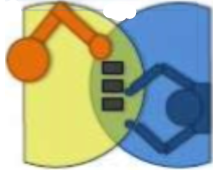
\includegraphics[height=1cm]{./bilder/MRKarten2}
    \begin{itemize}
        \item Externe Sensorik und Sicherheitssteuerung
        \item keine Trenneinrichtung
    \end{itemize}
\end{minipage}
\begin{minipage}[t]{0.33\linewidth}
    \textbf{Kollaboration}\hfill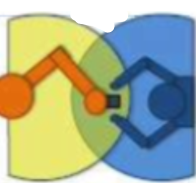
\includegraphics[height=1cm]{./bilder/MRKarten3}
    \begin{itemize}
        \item Integration Sensortechnik zur Leistungs und Kraftbegrenzung
        \item Begrenzung von Kraf bei Kollision
    \end{itemize}
\end{minipage}
\end{minipage}
\begin{tabular}{lll}
    \multirow{2}{3cm}{\textbf{MRK}}&\textbf{Unterschidliche}&\textbf{Gleiche}\\
                &\textbf{Arbeitsräume}&\textbf{Arbeitsräume}\\ \hline
    Sequentielle Bearbeitung& Keine Interaktion& Kooperation\\
    Gleichzeitige Bearbeitung & Koexistenz& Kollaboration\\
\end{tabular}

\subsection{Arten der Kooperation}
\begin{minipage}{0.5\linewidth}
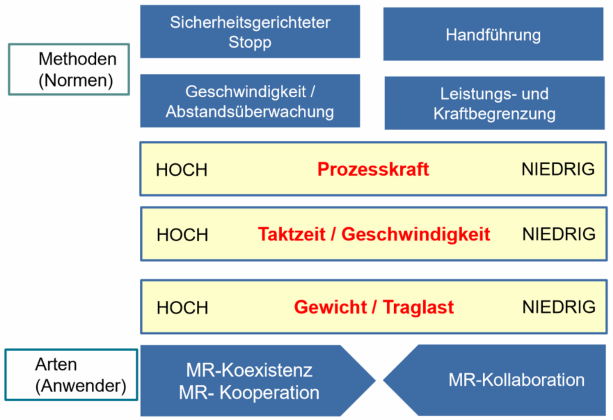
\includegraphics[width=0.8\linewidth]{./bilder/ArtenKooperation}
\end{minipage}
\begin{minipage}{0.5\linewidth}
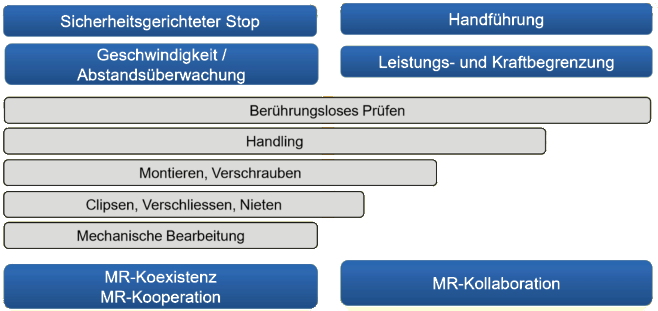
\includegraphics[width=\linewidth]{./bilder/ArtenAnwendungen}
\end{minipage}
\subsection{Kritische Rahmen- / Randbedingungen}
\begin{minipage}{0.5\linewidth}
    \subsubsection{Zykluszeit}
    \begin{itemize}
        \item Sicherheitsbewertete reduzierte Geschwindigkeit 250mm/s
        \item zusätzliche Sicherheitseinrichtung
        \item (In-)Direkte Abhängige Kraft via Geschwindigkeit
        \begin{itemize}
            \item Risikoanalyse, Distanz, Nutzlast, bewegte Robotermasse, Geschwindigkeit
        \end{itemize}
        \item Produktionssteigerung durch Erhöhung der Verfahrensgeschwindigkeit nachträglich möglich
    \end{itemize}
\end{minipage}
\begin{minipage}{0.5\linewidth}
    \subsubsection{Nutzlast/Werkstück}
    \begin{itemize}
        \item hat direkten Einfluss auf bewegte Robotermasse
        \item Direkte Abhängigkeit mit Kraft
        \begin{itemize}
            \item Risikoanalyse, Distanz, Nutzlast, bewegte Robotermasse, Geschwindigkeit
        \end{itemize}
        \item Die grösse kann einfluss auf die Distanz: Handflansch - Schwerpunkt haben
        \item Werkstück-Beschaffenheit wichtig $\rightarrow$ keine scharfen Kanten
    \end{itemize}
\end{minipage}
\begin{minipage}{0.5\linewidth}
    \subsubsection{Arbeistraum/ Interaktion}
    \begin{itemize}
        \item MRK Applikation kann jederzeit durch Kontakt/Eindringen in AR unterbrochen werden
        \item Prozess muss damit umgehen können $\rightarrow$ Reaktion programmieren
        \item Interaktion mit Menschen so eindeutig wie möglich
    \end{itemize}
\end{minipage}
\begin{minipage}{0.5\linewidth}
    \subsubsection{Mehrfacheinsatz}
    \begin{itemize}
        \item Fehlen fester Schutzeinrichtung und "`leichte"' Roboter machen Mehrfacheinsätze interessant
        \item Risikobeurteilung und -management bei (Wieder-)Inbetriebnahme, speziell der Sicherheitseinrichtung, sehr wichtig
    \end{itemize}
\end{minipage}
\subsubsection{Sicherheitsanforderungen}
\begin{itemize}
    \item Es kann zu Kontakt zwischen Roboter und Menschen kommen $\rightarrow$ Sicherheit muss gewährleistet sein
    \item Je nach Methode unterschiedliche Normen
    \item Auf die Sicherheitsanforderung kann einfluss genommen werden durch:
    \begin{itemize}
        \item Applikatio ohne Quetsch- und Druckpunkte
        \item Reduktion der Masse der bewegten Roboterteile
        \item Reduktion der Geschwindigkeit
        \item Veränderung der Roobotergestaltung $\rightarrow$ Vergrösserung der Kontaktfläche
        \item Vermeidung von Kontakt mit sensiblen Körperregionen
    \end{itemize}
\end{itemize}



\clearpage
\section{Robotermanipulation}
\subsection{Definition}
\begin{minipage}[t]{0.5\linewidth}
    \textbf{Effektor}\newline
    ist Teil des Handhabungsgeräts. Er wird am Handgelenk befestigt und an Energie und Steuerleitungen angeschlossen.
\end{minipage}
\begin{minipage}[t]{0.5\linewidth}
    \textbf{Greifer}\newline
    Ein Greifer ist das jenige Subsystem eines Industrieroboters, das eine 
    begrenzte Anzahl von geometrisch bestimmten Werkstücken für einen 
    bestimmten Zeitraum hält, d.h. die Position und Orientierung dieser 
    Werkstücke relativ zum Werkzeug-Koordinatensystem sichert.
\end{minipage}
\subsection{Hauptfunktion Greifer}
\begin{minipage}{0.5\linewidth}
\begin{itemize}
    \item Vorbereiten eines Kontakts
    \begin{itemize}
        \item bekannte Objektpositon und Orientirung erreichen
    \end{itemize}
    \item Herstellung des Kontakts zwischen Objekt und Greiffinger
    \item Manipulation des Objekts mit dem Greifer
        \begin{itemize}
        \item Ortsveränderung, Drehung, Montieren
    \end{itemize}
    \item Ablegen des Greifobjekts durch lösen des Kontakts
\end{itemize}
\end{minipage}
\begin{minipage}{0.5\linewidth}
    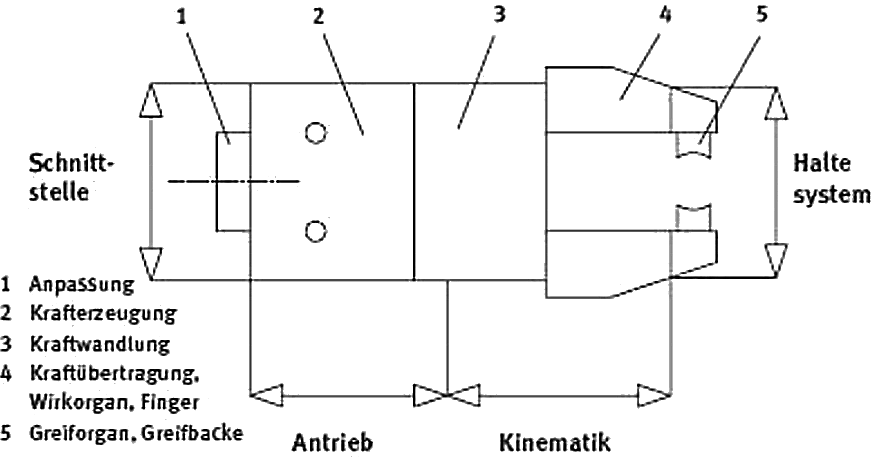
\includegraphics[width=\linewidth]{./bilder/Greifer}
\end{minipage}
\begin{minipage}{\linewidth}
    \subsection{Lösungsfindung für den Greifer}
    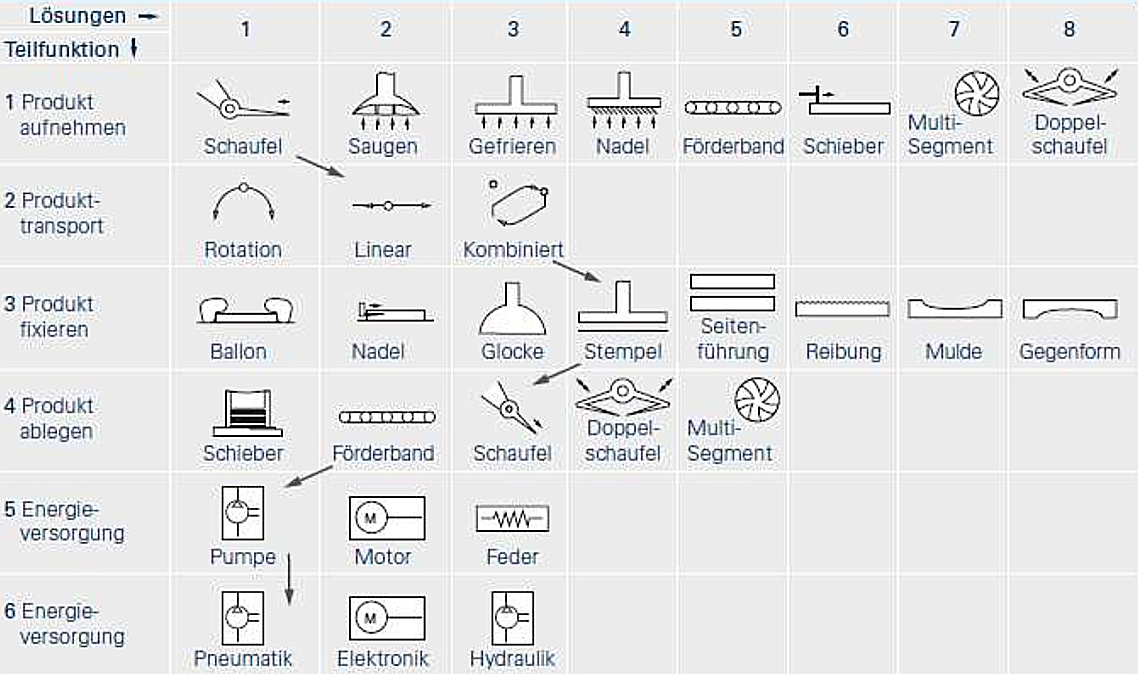
\includegraphics[width=0.9\linewidth]{./bilder/GreiferLosung}
\end{minipage}
\begin{minipage}{0.5\linewidth}
    \subsection{Last}
    \begin{itemize}
        \item Effektrolast
        \begin{itemize}
            \item Last die \textbf{als} Werkzeug oder Greifer angebracht ist
        \end{itemize}
        \item Nutzlast
        \begin{itemize}
            \item Last, welche zusätzlich zur Effektorlast bewegt werden kann ohne das daraus Einschränkungen in Geschwindigkeit, Beschleunigung oder Genauigkeit entstehen
        \end{itemize}
    \end{itemize}
\end{minipage}
\begin{minipage}{0.5\linewidth}
    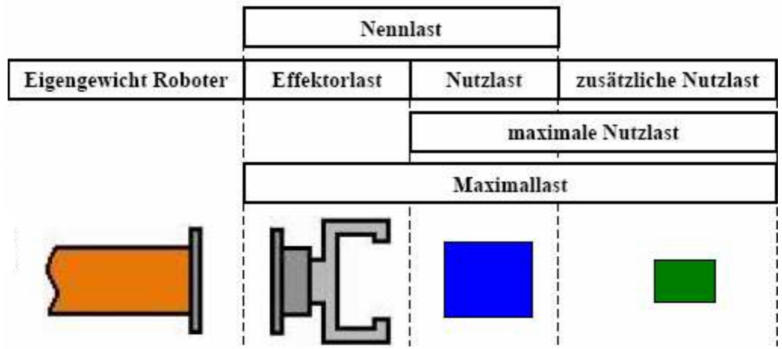
\includegraphics[width=\linewidth]{./bilder/RobLast}
\end{minipage}
\clearpage
\subsubsection{Nutzlast bei verschiedenen Roboterkinematiken}
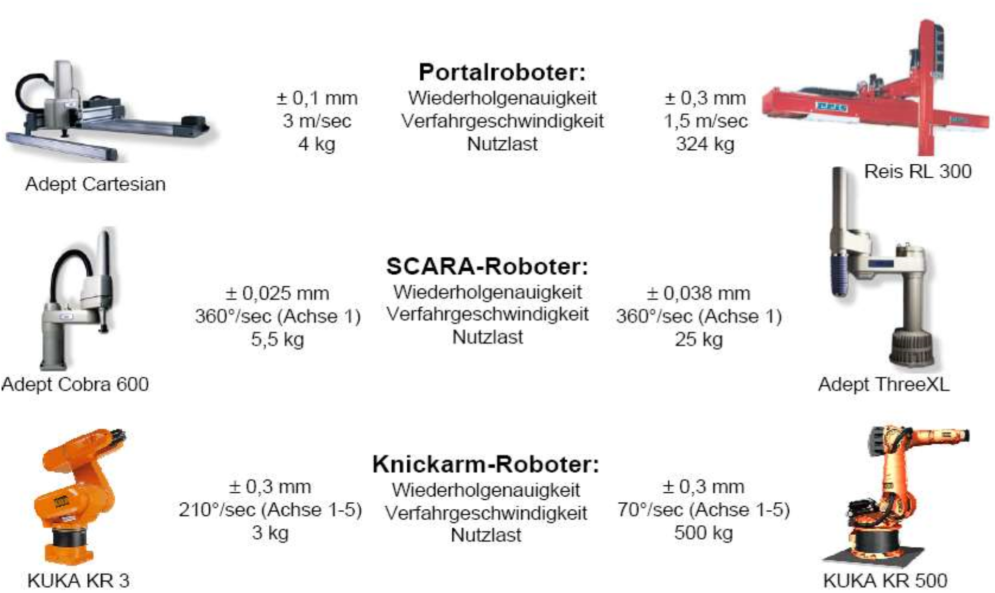
\includegraphics[width=1\linewidth]{./bilder/RobLastdiffKin}
\enlargethispage{3\baselineskip}
\subsection{Greifer}
\raisebox{-1\height}{
\begin{minipage}{0.5\linewidth}  
    \subsubsection{Halteprinzipien}
    \includegraphics[width=\linewidth]{./bilder/HalteprinzGreif}
\end{minipage}}\hspace{0.09\linewidth}
\begin{minipage}[t]{0.4\linewidth}
    \subsubsection{Gliederung nach Wirkprinzip}
        \textbf{Mechanischer Greifer}
        \begin{itemize}
            \item Zangengreifer
            \item Klemmgreifer
            \item Gelenkgreifer
            \item Verhakende Greifer
            \begin{itemize}
                \item Klettgreifer
                \item Nadelgreifer
            \end{itemize}
        \end{itemize}

        \textbf{Pneumatische Greifer}
        \begin{itemize}
            \item Überdruckgreifer
            \begin{itemize}
                \item Lochgreifer
                \item Zypfengreifer
                \item Schrumpfringgreifer
                \item Luftstrahlgreider
                \item Membrangreider
            \end{itemize}
        \end{itemize}

        \textbf{Pneumostatische Pneumodynamische}
        \begin{itemize}
            \item Unterdruckgreifer
            \begin{itemize}
                \item Vakuumsauger
                \item Haftsauger
                \item Luftstromgreifer
            \end{itemize}
        \end{itemize}

        \textbf{Elektrische Greifer}
        \begin{itemize}
            \item Magnetgreifer
            \item Elektrostatische Greifer
        \end{itemize}
           
        \textbf{Adhäsove Greifer}
        \begin{itemize}
            \item Kapilargreifer
            \item Gefriefgreifer
            \item Klebstoffgreifer
        \end{itemize}
\end{minipage}
\clearpage

\begin{multicols}{2}
    \subsubsection{Anforderungen}
    \begin{itemize}
        \item Greifkraft
        \item Baugrösse
        \begin{itemize}
            \item Unnötoge Störkonturen vermeiden
            \item möglichst klein/kompakt
        \end{itemize}
        \item Anschlussmöglichkeiten
        \begin{itemize}
            \item Fixiermöglichkeit für wiederholgenauen Austausch
        \end{itemize}
        \item Schnittstelle Greifer
        \begin{itemize}
            \item Exakte, spielfreie, verdrehsichere Aufnahme
            \item Schlupffreie Übertragung der Kräfte und Momente
            \item Verlustfreie Übertragung (pneu.,el.,hyd. Energie) auf Antrieb
        \end{itemize}
        \item Greifergewicht
        \begin{itemize}
            \item EInfluss auf Traglast
        \end{itemize}
        \item Greifkraftsicherung
        \begin{itemize}
            \item Bei Energieausfall muss die Spannkraft des Greifers erhalten bleiben und Handhabungsobjekt sichern
        \end{itemize}
        \item Greiferlebensdauer
        \begin{itemize}
            \item Einflussfaktoren: Lebensdrauer der Fertigungstoleranz, Fingerlänge, Kühlschmiermittel, Taktzahlen, Wartung, äussere Kräfte, Temperatur, kinemat. Wirkprinzip
        \end{itemize}
        \item Öffnungs- und Schliesszeiten
        \item Wartungsarm
        \item Schmutzunempfindlich    
    \end{itemize}
\end{multicols}
\begin{minipage}{0.5\linewidth}
    \subsection{Sauggreifer}
    \begin{itemize}
        \item Kraftschluss wird durch unterschiedliche Druckverhältnisse erzeugt
        \item Arten/Prinzip
        \begin{itemize}
            \item Vakuumsauger $\rightarrow$ Vakuumpumpe
            \item Luftstromsauger $\rightarrow$ Venturidüse
            \item Haftsauger $\rightarrow$ Saugnapf anpressen
        \end{itemize}
        \item Einsatzgebiete
        \begin{itemize}
            \item Haftsauger $\rightarrow$ glatte, luftundurchlässige Werkstückoberflächen
            \item Vakuum- Luftstromsauger $\rightarrow$ weniger glatte bis raue und poröse Oberflächen
        \end{itemize}
        \item Haltekraft
        \begin{itemize}
            \item[] $ F_h=A\cdot p_u$
            \item[] $ p_u= \frac{m\cdot g}{A \cdot \eta}$
            \item[] $F_h$= Haltekraft [N],$A$= Fläche [$cm^2$]
            \item[] $p_u$=Unterdruck [$N/cm^2$], $\eta$=dyn. Viscosität [$kg/(m\cdot s)$]
            \item[] Haltrekraft mal Sicherheitsfaktor 2
        \end{itemize}
    \end{itemize}

\includegraphics[width=\linewidth]{./bilder/GreiferAuswahl}
\end{minipage}
\begin{minipage}{0.5\linewidth}
    \vspace{-2cm}
    \subsection{Mechanische Greifer}
        \begin{itemize}
            \item Einfinger-, Zweifinger- oder Mehrfinger Ausführung
            \item Starr-, Starr-gelenkiger- oder elastischer Ausführung
            \item Antrieb erfolgt mechanisch, pneumatisch oder elektrisch
        \end{itemize}
    \begin{center}
     \textbf{Greifkraft beim Abheben}\hfill\null
    \[ \qquad F_G=\frac{m \cdot (g + a) \cdot S}{\mu \cdot n} \]
    \textbf{Greifkraft beim Querhub}\hfill\null
    \[ \qquad F_G=\frac{m \cdot g \cdot S}{\mu \cdot n} + m \cdot a \]
    \end{center}

        Max. Greifkraft bei NOT-AUS nötig.
        
    \begin{minipage}{0.3\linewidth}
    \includegraphics[width=\linewidth]{./bilder/GreiferAusfurung}
    \end{minipage}
    \begin{minipage}{0.7\linewidth}
    $n$: Anz. Greifbacken\newline
    $\mu$: Reibkoeff. Greifer zu WS\newline
    $m$: Masse des WS [kg]\newline
    $a$: Beschleunigung der dyn. Bewegung [$m/s^2$]\newline
    $S$: Sicherheitsfaktor\newline
    $g$: Erdbeschleunigung 9.81[$m/s^2$]
    \end{minipage}
\end{minipage}

\begin{minipage}{0.5\linewidth}
    Kräftesituation bei bewegtem Greifer:
    \begin{enumerate}[label=\alph*)]
        \item Ruhezustand
        \item Aufwärtsbewegung
        \item Abwärtsbewegung
        \item Querbewegung
        \item Schrägfahrt aufwärts
    \end{enumerate}
\end{minipage}
\begin{minipage}{0.5\linewidth}
    \vspace{-2cm}
    \includegraphics[width=\linewidth]{./bilder/GreiferKraft}
\end{minipage}


\subsection{Sensorik}
\begin{minipage}{0.5\linewidth}
    \subsubsection{Ziele}
   \begin{itemize}
       \item Abstandserkennung zwischen Obj. und Greifer
       \item Objektkontakt am Greifer
       \item Objekt im Greifer?
       \item Objekt korrekt gegriffen?
       \item rutscht das Objet vom Greifer?
   \end{itemize}
\end{minipage}
\begin{minipage}{0.5\linewidth}
    \subsubsection{Typische Sensoren}
    \begin{itemize}
        \item Videokameras (oft s/w)
        \item Ultraschallsensor (Rechtwinklig)
        \item Laser oder IR- Distanzsensoren
        \item Induktive Sensoren (kleine Distanzen)
        \item Lichtschranke oder Induktive Senosoren
        \item Kraft-/Momentsensoren am Greifer
    \end{itemize}
\end{minipage}
 \includegraphics[width=\linewidth]{./bilder/GreiferZyklus}
 
 \subsubsection{Kamerasysteme}
 \begin{tabular}{p{5cm}p{6cm}p{6cm}}
    \textbf{Stationäre Kamera}\newline
    Transformation vom Kamera-KS ins Basis-KS&
    \begin{itemize}
        \item[+] Ist keine Last für den Roboter
    \end{itemize}
    &
    \begin{itemize}
        \item[-] Messgenauigkeit begrenzt, da die Kamera relativ weit weg vom Objekt ist.
        \item[-] Roboter evt. im Blickfeld
        \item[-] Vermessung des Kamerasichtfeldes
    \end{itemize}\\
    \textbf{Bewegte Kamera}\newline
    Transformation vom Kamera-KS ins Werkzeug-KS&
    \begin{itemize}
        \item[+] Gute Messgenauigkeit, da nah am Objekt
        \item[+] Kein grosses Sichtfeld nötig
        \item[+] Keine Tragkonstrukiton für die Kamerafixierung notwendig.
    \end{itemize}&
    \begin{itemize}
        \item[-] Werkzeug evt. im Bild
        \item[-] Kamera kann durch Kollision beschödigt werden.
        \item[-] Kameragewicht am Werkzeug reduziert Traglast.
    \end{itemize}\\
 \end{tabular}

        \textbf{Kalibrierung:}\newline
        Das Bildverarbeitungssystem liefert die Werkstückdaten bezgl. des Kamerakoordsys. Für die Umrechnung muss eine Vermessung des Kamerasichtsfelds im Arbeitsraum erfolgen. 
        Dies kann bsp. mit zwei kreisförmigen Scheiben erfolgen deren Position im Basis-Koordsys. bekannt sind und danacha im Kamera-Koordsys. ermittelt werden. So kann die TF ermittelt werden.
        Ist die Kammera am Werkzeug montiert soll die TF zwischen Kamera-Koordsys. und Werkzeugkoordsys. erfolgen.
        \clearpage
        
 \includegraphics[width=\linewidth]{./bilder/GreiferProject}
\clearpage
%\section{Wichtige Formeln}
	$\sin^2(b)+\cos^2(b)=1 \qquad \tan(b)=\frac{\sin(b)}{\cos(b)}$

\subsection{Funktionswerte für Winkelargumente}
	\renewcommand{\arraystretch}{1.5}
	\begin{minipage}{5cm}
		\begin{tabular}[c]{ |c|c||c|c|c| }
	    	\hline
			deg & rad & sin & cos & tan\\
			\hline
			0\symbol{23} & 0 & 0 & 1 & 0\\
			\hline
			30\symbol{23} & $\frac{\pi}{6}$ & $\frac{1}{2}$ & $\frac{\sqrt{3}}{2}$ &
			$\frac{\sqrt{3}}{3}$\\
			\hline
			45\symbol{23} & $\frac{\pi}{4}$ & $\frac{\sqrt{2}}{2}$ & $\frac{\sqrt{2}}{2}$
			& 1\\
			\hline
			60\symbol{23} & $\frac{\pi}{3}$ & $\frac{\sqrt{3}}{2}$ & $\frac{1}{2}$ &
			$\sqrt{3}$\\
			\hline			
		\end{tabular}			
	\end{minipage}
	\begin{minipage}{4.3cm}
		\begin{tabular}[c]{ |c|c||c|c|}
	    	\hline
			deg & rad & sin & cos\\
			\hline
			90\symbol{23} & $\frac{\pi}{2}$ & 1 & 0\\
			\hline	
			120\symbol{23} & $\frac{2\pi}{3}$ & $\frac{\sqrt{3}}{2}$ & $-\frac{1}{2}$ \\
			\hline
			135\symbol{23} & $\frac{3\pi}{4}$ & $\frac{\sqrt{2}}{2}$ & $-\frac{\sqrt{2}}{2}$\\
			\hline
			150\symbol{23} & $\frac{5\pi}{6}$ & $\frac{1}{2}$ & $-\frac{\sqrt{3}}{2}$\\
			\hline
		\end{tabular}			
	\end{minipage}
	\begin{minipage}{4.5cm}
		\begin{tabular}[c]{ |c|c||c|c| }
	    	\hline
			deg & rad & sin & cos\\
			\hline
			180\symbol{23} & $\pi$ & 0 & -1\\
			\hline	
			210\symbol{23} & $\frac{7\pi}{6}$ & $-\frac{1}{2}$ & $-\frac{\sqrt{3}}{2}$\\
			\hline
			225\symbol{23} & $\frac{5\pi}{4}$ & $-\frac{\sqrt{2}}{2}$ & $-\frac{\sqrt{2}}{2}$\\
			\hline
			240\symbol{23} & $\frac{4\pi}{3}$ & $-\frac{\sqrt{3}}{2}$ & $-\frac{1}{2}$\\
			\hline
		\end{tabular}			
	\end{minipage}
	\begin{minipage}{4.5cm}
		\begin{tabular}[c]{ |c|c||c|c| }
	    	\hline
			deg & rad & sin & cos\\
			\hline
			270\symbol{23} & $\frac{3\pi}{2}$ & -1 & 0\\
			\hline	
			300\symbol{23} & $\frac{5\pi}{3}$ & $-\frac{\sqrt{3}}{2}$ & $\frac{1}{2}$\\
			\hline
			315\symbol{23} & $\frac{7\pi}{4}$ & $-\frac{\sqrt{2}}{2}$ & $\frac{\sqrt{2}}{2}$\\
			\hline
			330\symbol{23} & $\frac{11\pi}{6}$ & $-\frac{1}{2}$ & $\frac{\sqrt{3}}{2}$\\
			\hline
		\end{tabular}			
	\end{minipage}
	\renewcommand{\arraystretch}{1}
	
	\subsection{Periodizität}
	$\cos(a+k\cdot2\pi)=\cos(a) \qquad \sin(a+k\cdot2\pi)=\sin(a) \qquad
	(k \in \mathbb{Z})$
	
\subsection{Quadrantenbeziehungen}
	\begin{tabbing}
     	xxxxxxxxxxxxxxxxxxxxxxxxxxxxxxxxxx \= \kill
	  	$\sin(-a)=-\sin(a)$ \> $\cos(-a)=\cos(a)$\\
		$\sin(\pi - a)=\sin(a)$ \> $\cos(\pi - a)=-\cos(a)$\\
		$\sin(\pi + a)=-\sin(a)$ \> $\cos(\pi +a)=-\cos(a)$\\
		$\sin\left(\frac{\pi}{2}-a \right)=\sin\left(\frac{\pi}{2}+a \right)=\cos(a)$ \>
		$\cos\left(\frac{\pi}{2}-a \right)=-\cos\left(\frac{\pi}{2}+a \right)=\sin(a)$  
    \end{tabbing}


\begin{minipage}{12.5cm}
	\subsection{Additionstheoreme}
		$\sin(a \pm b)=\sin(a) \cdot \cos(b) \pm \cos(a) \cdot \sin(b)$\\
		$\cos(a \pm b)=\cos(a) \cdot \cos(b) \mp \sin(a) \cdot \sin(b)$\\	
		$\tan(a \pm b)=\frac{\tan(a) \pm \tan(b)}{1 \mp \tan(a) \cdot \tan(b)}$
		
	\subsection{Doppel- und Halbwinkel}	
		$\sin(2a)=2\sin(a)\cos(a)$\\
		$\cos(2a)=\cos^2(a)-\sin^2(a)=2\cos^2(a)-1=1-2\sin^2(a)$\\
		$\cos^2 \left(\frac{a}{2}\right)=\frac{1+\cos(a)}{2} \qquad
		\sin^2 \left(\frac{a}{2}\right)=\frac{1-\cos(a)}{2}$ \\ 
	\subsection{Summe, Differenz und Produkte}
	\begin{minipage}{7.5cm}	
		$\sin(a)+\sin(b)=2 \cdot \sin \left(\frac{a+b}{2}\right) \cdot
		\cos\left(\frac{a-b}{2}\right)$\\
		$\sin(a)-\sin(b)=2 \cdot \sin \left(\frac{a-b}{2}\right) \cdot
		\cos\left(\frac{a+b}{2}\right)$\\
		$\cos(a)+\cos(b)=2 \cdot \cos \left(\frac{a+b}{2}\right) \cdot
		\cos\left(\frac{a-b}{2}\right)$\\
		$\cos(a)-\cos(b)=-2 \cdot \sin \left(\frac{a+b}{2}\right) \cdot
		\cos\left(\frac{a-b}{2}\right)$\\
		$\tan(a) \pm \tan(b)=\frac{\sin(a \pm b)}{\cos(a)\cos(b)}$	\\
	\end{minipage}
	\begin{minipage}{6cm}
		$\sin(a)\sin(b)=\frac{1}{2}(\cos(a-b)-cos(a+b))$\\
		$\cos(a)\cos(b)=\frac{1}{2}(\cos(a-b)+cos(a+b))$\\
		$\sin(a)\cos(b)=\frac{1}{2}(\sin(a-b)+\sin(a+b))$\\
	\end{minipage}	
	
	\subsection{Differentialrechnung}
	\begin{minipage}{5cm}
    $ a \Longrightarrow 0$ \space $[a=const.]\\
    x \Longrightarrow 1 \\
    sin(x)\Longrightarrow cos(x) \\
    cos(x)\Longrightarrow -sin(x) \\
    tan(x)\Longrightarrow \frac{1}{cos^{2}(x)} \\
    $
    \end{minipage}
	\begin{minipage}{6cm}
    $ (u+v-w)' = u'+v'-u' \\
    (au)'= au'$ \space $ [a=const.]\\
    (uv)'=u'v + uv' \\
    (\frac{u}{v})' = \frac{vu'-uv'}{v^{2}} \\
    (u(v(y(x))))' = u'(v)v'(y)y'(x) \\
    $
    \end{minipage}
    	
\end{minipage}

%\clearpage
\section{Symbole und Theorie}



	\subsection{Übersicht von Skript und Übungen}
	\includegraphics[width=10cm]{./bilder/uebersicht.png}
\clearpage
\addtocontents{toc}{\setcounter{tocdepth}{1}} %ToC ohnly shows section
\section{Idiotenseite}
%\subsection{Diverses}
\begin{tabbing}
	xxxxxxxxxxxxxxxxxxxxxxxxxxxx \= xxxxxxxxxxxxxxxxxxxxxxxxxxxxxx \= \kill
 	$f'(z) = \lim \limits_{\Delta z \rightarrow 0} \frac{f(z + \Delta z) -
	f(z)}{\Delta z}$ \> $(a + b)^n = \sum_{k=0}^{n} \binom n k a^{n-k} \cdot b^k$ \>
	$(a \pm b)^3 =a^3 \pm  3 a^{2} b + 3 a b^2 \pm b^3 $\\ \\
	$x_{1,2} = \dfrac{-b \pm \sqrt{b^2 - 4ac}}{2a}$ \> $\binom n k = \dfrac{n!}{k!
	\cdot (n-k)!}$ \> $(a \pm b)^4 =a^4 \pm  4 a^{3} b + 6a^2b^2 \pm 4 a b^3 +
	b^4$\\
\end{tabbing}
%\subsection{Reihenentwicklungen}
\begin{tabular}{llll}
\textbf{Geometrische Reihe}
	& $\sum\limits_{n=0}^{\infty} x^n$ 
	& $= \dfrac{1}{1-x}$
	& $|x| < 1$ \\
	
	& $\sum\limits_{k=0}^{\infty} k \, x^k$ & $= x \sum\limits_{k=1}^{\infty} k \,
	x^{k-1} = \dfrac{x}{(1-x)^2} $ 
	& $x \neq 1$ \\
    & $\sum\limits_{k=0}^{n} a_0\cdot q^k$ & $= a_0 \dfrac{1-q^{n+1}}{1-q}$
    & $q \neq 1$\\
\textbf{Binominalreihe} 
	& $\sum\limits_{n=0}^\infty \binom{\alpha}{n} x^n $ &$= (1+x)^\alpha$
	& $x \in (-1,1)$ \\
\textbf{E-Funktion}
	& $\sum\limits_{k = 0}^{\infty} \dfrac{x^k}{k!}$ &$ = e^x$
	& 
\end{tabular}

%\subsection{Kurven}
\begin{multicols}{4}
\subsubsection{e-Funktion}
\includegraphics[width=4.5cm]{idiotenseite/images/Exp.png}
\subsubsection{Sinus-Funktion}
\includegraphics[width=4.5cm]{idiotenseite/images/sin.png}
\subsubsection{Cosinus-Funktion}
\includegraphics[width=4.5cm]{idiotenseite/images/cos.png}
\subsubsection{Tangens-Funktion}
\includegraphics[width=4.5cm]{idiotenseite/images/tan.png}
\end{multicols}
\subsection{SI-Vorsätze}
\renewcommand{\arraystretch}{1.2}
\begin{tabularx}{\textwidth}{|X|X|X|X|X|X|l|}
	\hline
\textbf{Symbol}	&\textbf{Name}  &\textbf{Wert}  &\textbf{Binär}  &\textbf{Symbol}  &\textbf{Name}  &\textbf{Wert}
 \\ \hline 
da	& Deka    &$ 10^1 $   &    			     & d          & Dezi   &$ 10^{-1} $ 
\\ \hline
h	&Hekto    &$ 10^2 $   &                  & c          & Centi  &$ 10^{-2} $ 
\\ \hline
k	&Kilo     &$ 10^3 $   &$ 2^{10}=1024  $  & m          & Mili   &$ 10^{-3} $ 
\\ \hline
M	& Mega    &$ 10^6 $   &$ 2^{20} $        &$ y, \mu $  & Mikro  &$ 10^{-6} $
\\ \hline
G   &Giga     &$ 10^9 $   &$ 2^{30} $        & n          & Nano   &$ 10^{-9} $ 
\\ \hline
T	& Tera    &$ 10^{12} $&$ 2^{40} $        & p          & Piko   &$ 10^{-12} $
\\ \hline
P	&Peta	  &$ 10^{15} $&$ 2^{50} $	     & f          &	Femto  &$ 10^{-15} $
\\ \hline
\end{tabularx} 

%\subsection{GrichischesAlphabet}
\begin{multicols}{2}
	\subsubsection{klein}
	\begin{tabular}{ |l|l|l|l|l|l|l|l|}
		\hline
		$\alpha$&Alpha&$\theta$&Theta&o&o&$\tau$&Tau\\
		\hline
		$\beta$&Beta&$\vartheta$&Theta&$\pi$&Pi&$\upsilon$&Ypsilon\\
		\hline
		$\gamma$&Gamma&$\gamma$&Gamma&$\varpi$&Pi&$\phi$&Phi\\
		\hline
		$\delta$&Delta&$\kappa$&Kappa&$\rho$&Roh&$\varphi$&Phi\\
		\hline
		$\epsilon$&Epsilon&$\lambda$&Lambda&$\varrho$&Roh&$\chi$&Chi\\
		\hline
		$\varepsilon$&Epsilon&$\mu$&Mu&$\sigma$&Sigma&$\psi$&Psi\\
		\hline
		$\zeta$&Zeta&$\nu$&Nu&$\varsigma$&Sigma&$\omega$&Omega\\
		\hline
		$\eta$&Eta&$\xi$&Xi&&&&\\
		\hline
	\end{tabular}
	\columnbreak
	
	\subsubsection{gross}
	\begin{tabular}{|l|l|l|l|l|l|l|l|}
		\hline
		$\Gamma$&Gamma&$\Lambda$&Lambda&$\Sigma$&Sigma&$\Psi$&Psi\\
		\hline
		$\Delta$&Delta&$\Xi$&Xi&$\Upsilon$&Ypsilon&$\Omega$&Omega\\
		\hline
		$\Theta$&Theta&$\Pi$&Pi&$\Phi$&Phi&&\\
		\hline
	\end{tabular}
\end{multicols}
\begin{sidewaystable}
\subsection{Einige unbestimmte Integrale\formelbuch{1074}}
\label{unbestimmte_integrale}
\begin{tabular}{|p{12cm}|p{12cm}|}
  \hline
  
    $ \int dx=x+C $ &
     $ \int{x^\alpha}dx=\frac{x^{\alpha+1}}{\alpha+1}+C,\ x \epsilon \mathbb
    R ^+,\ \alpha \epsilon \mathbb R \backslash \{ -1 \} $ \\\hline
     $ \int{\frac{1}{x}}dx=\ln \left| x \right| + C,\ x\neq0 $ &
     $ \int{e^x}dx=e^x+C $ \\\hline
     $ \int{a^x}dx=\frac{a^x}{\ln{a}}+C,\ a \epsilon \mathbb 
    R^+\backslash\{1\} $ &
     $ \int{ \sin{x}} dx = -\cos{x} + C $ \\\hline
     $ \int{\cos{x}} dx = \sin{x} + C $ &
     $ \int{\frac{dx}{\sin^2x}}=-\cot{x}+C,\ x\neq k\pi\ \mathrm{mit}\ k
    \epsilon \mathbb Z $ \\\hline
     $ \int{\frac{dx}{\cos^2x}}=\tan{x}+C,\ x\neq\frac{\pi}{2}+k\pi\
    \mathrm{mit} k \epsilon \mathbb Z $ & 
    
    %10. :
     $ \int{\sinh{x}}dx = \cosh{x}+C $ \\ \hline
     $ \int{\cosh{x}}dx = \sinh{x}+C $ &
     $ \int{\frac{dx}{\sinh^2x}}=-\coth{x}+C,\ x\neq0 $ \\\hline
     $ \int{\frac{dx}{\cosh^2x}}=\tanh{x}+C $ &
     $ \int{\frac{dx}{ax+b}} = \frac{1}{a}\ln \left|ax + b\right| + C,\
    a\neq 0,x\neq-\frac{b}{a} $ \\\hline
     $ \int{\frac{dx}{a^2x^2+b^2}}=\frac{1}{ab}\arctan{\frac{a}{b}x}+C,\
    a\neq0,\ b\neq0 $ &
     $
    \int{\frac{dx}{a^2x^2-b^2}}=\frac{1}{2ab}\ln{\left|\frac{ax-b}{ax+b}\right|}+C,\
    a\neq0,\ b\neq0,\ x\neq\frac{b}{a},\ x\neq-\frac{b}{a} $ \\\hline
     $
    \int{\sqrt{a^2x^2+b^2}}dx=\frac{x}{2}\sqrt{a^2x^2+b^2}+\frac{b^2}{2a}\ln{(ax+\sqrt{a^2x^2+b^2})}+C,\
    a\neq0,\ b\neq0 $ &
     $
    \int{\sqrt{a^2x^2-b^2}}dx=\frac{x}{2}\sqrt{a^2x^2-b^2}-\frac{b^2}{2a}\ln\left|ax+\sqrt{a^2x^2-b^2}\right|+C,\
    a\neq0,\ b\neq0,a^2x^2\geqq b^2$ \\\hline
     $
    \int\sqrt{b^2-a^2x^2}dx=\frac{x}{2}\sqrt{b^2-a^2x^2}+\frac{b^2}{2a}\arcsin\frac{a}{b}x+C,\
    a\neq0,\ b\neq0,\ a^2x^2\leqq b^2 $ &
    %20.:
     $
    \int\frac{dx}{\sqrt{a^2x^2-b^2}}=\frac{1}{a}\ln(ax+\sqrt{a^2x^2+b^2})+C,\
    a\neq0,\ b\neq0 $ \\\hline
     $
    \int\frac{dx}{\sqrt{a^2x^2-b^2}}=\frac{1}{a}\ln\left|ax+\sqrt{a^2x^2-b^2}\right|+C,\
    a\neq0,\ b\neq0,\ a^2x^2>b^2 $ &
     $ \int\frac{dx}{\sqrt{b^2-a^2x^2}}=\frac{1}{a}\arcsin\frac{a}{b}x+C,\
    a\neq0,\ b\neq0,\ a^2x^2<b^2 $ \\\hline
     Die Integrale $\int\frac{dx}{X}, \int\sqrt{X}dx,
    \int\frac{dx}{\sqrt{X}}$ mit $X=ax^2+2bx+c,\ a\neq0 $ werden durch 
    die Umformung $X=a(x+\frac{b}{a})^2+(c-\frac{b^2}{a}) $ und die
    Substitution $ t=x+\frac{b}{a} $ in die oberen 4 Zeilen
    transformiert. & $ \int\frac{xdx}{X}=\frac{1}{2a}\ln\left|X\right|-\frac{b}{a}\int\frac{dx}{X},\
    a\neq0,\ X=ax^2+2bx+c $ \\\hline
     $ \int\sin^2axdx=\frac{x}{2}-\frac{1}{4a}\cdot\sin2ax+C,\ a\neq0 $ &
     $ \int\cos^2axdx=\frac{x}{2}+\frac{1}{4a}\cdot\sin2ax+C,\ a\neq0 $ \\\hline
     $ \int\sin^naxdx=-\frac{sin^{n-1}ax\cdot\cos
    ax}{na}+\frac{n-1}{n}\int\sin^{n-2}axdx,\ n \epsilon \mathbb N,\ a\neq0 $ &
     $ \int\cos^naxdx=\frac{\cos^{n-1}ax\cdot\sin
    ax}{na}+\frac{n-1}{n}\int\cos^{n-2}axdx,\ n\epsilon \mathbb N,\ a\neq0 $
    \\\hline
     $ \int\frac{dx}{\sin ax} =
    \frac{1}{a}\ln\left|\tan\frac{ax}{2}\right|+C,\ a\neq0,\ x\neq
    k\frac{\pi}{a}\ \mathrm{mit}\ k\epsilon\mathbb Z$ &
    %30.:
     $ \int\frac{dx}{\cos
    ax}=\frac{1}{a}\ln\left|\tan(\frac{ax}{2}+\frac{\pi}{4})\right|+C,\ a\neq0,\
    x\neq\frac{\pi}{2a}+k\frac{\pi}{a}\ \mathrm{mit}\ k\epsilon\mathbb Z $
    \\\hline
     $\int\tan axdx=-\frac{1}{a}\ln\left|\cos ax\right|+C,\ a\neq0,\
    x\neq\frac{\pi}{2a}+k\frac{\pi}{a} \mathrm{mit}\ k\epsilon\mathbb Z$ &
     $\int\cot axdx=\frac{1}{a}\ln\left|\sin ax\right|+C,\ a\neq0,\ x\neq
    k\frac{\pi}{a} \mathrm{mit} k\epsilon\mathbb Z $ \\ \hline
     $ \int x^n\sin axdx=-\frac{x^n}{a}\cos ax+\frac{n}{a}\int x^{n-1}\cos
    axdx,\ n\epsilon\mathbb N,\ a\neq0 $ &
    $ \int x^n\cos axdx=\frac{x^n}{a}\sin ax-\frac{n}{a}\int x^{n-1}\sin
    axdx,\ n\epsilon\mathbb N,\ a\neq0 $ \\ \hline
     $ \int x^ne^{ax}dx=\frac{1}{a}x^ne^{ax}-\frac{n}{a}\int
    x^{n-1}e^{ax}dx,\ n\epsilon\mathbb N,\ a\neq0 $ &
     $ \int e^{ax}\sin bxdx=\frac{e^{ax}}{a^2+b^2}(a\sin bx-b\cos bx)+C,\
    a\neq0,\ b\neq0 $  \\ \hline
     $ \int e^{ax}\cos bxdx=\frac{e^{ax}}{a^2+b^2}(a\cos bx + b\sin bx)+C,\
    a\neq0,\ b\neq0 $ &
     $ \int\ln x dx = x(\ln x-1)+C,\ x\epsilon\mathbb R^+ $ \\ \hline
     $ \int x^\alpha \cdot \ln xdx =
    \frac{x^{\alpha+1}}{(\alpha+1)^2}\lbrack(\alpha+1)\ln x-1\rbrack + C,\
    x\epsilon\mathbb R^+,\ \alpha\epsilon\mathbb R\backslash\{-1\} $ & \\ \hline
    %FF1 Seite 496
    
\end{tabular}
\end{sidewaystable}
%\begin{sidewaystable}
\subsection{Ableitungen elementarer Funktionen\formelbuch{436}}
\label{unbestimmte_integrale}
\renewcommand{\arraystretchOriginal}{2.5}
\begin{tabular}{|l|l||l|l|}
  \hline
  \textbf{Funktion} & \textbf{Ableitung} & \textbf{Funktion} &
  \textbf{Ableitung}\\\hline
  $C$ (Konstante) & 0 & $\sec x$ & $\dfrac{\sin x}{\cos^2 x}$ \\
  $x$ & 1 & $\sec^{-1} x$ & $\dfrac{-\cos x}{\sin^2 x}$\\
  $x^n$ ($n\in\mathbb{R}$) & $nx^{n-1}$ & $\arcsin x \quad (|x| < 1)$ &
  $\dfrac{1}{\sqrt{1-x^2}}$\\
  $\dfrac{1}{x}$ & $-\dfrac{1}{x^2}$ & $\arccos x \quad (|x| < 1)$ &
  $-\dfrac{1}{\sqrt{1-x^2}}$\\
  $\dfrac{1}{x^n}$ & $-\dfrac{n}{x^{n+1}}$ & $\arctan x$ & $\dfrac{1}{1+x^2}$\\
  $\sqrt{x}$ & $\dfrac{1}{2\sqrt{x}}$ & arccot $x$ & $-\dfrac{1}{1+x^2}$\\
  $\sqrt[n]{x}\quad (n\in\mathbb{R}, n \neq 0, x > 0)$ &
  $\dfrac{1}{n\sqrt[n]{x^{n-1}}}$ & arcsec $x$ & $\dfrac{1}{x\sqrt{x^2-1}}$\\
  $\mathrm{e}^x$ & $\mathrm{e}^x$ & arcossec $x$ & $-\dfrac{1}{x\sqrt{x^2-1}}$\\
  $\mathrm{e}^{bx}\quad (b\in\mathbb{R})$ & $b\mathrm{e}^{bx}$ & $\sinh x$ &
  $\cosh x$\\
  $a^x\quad (a > 0)$ & $a^x\ln a$ & $\cosh x$ & $\sinh x$\\
  $a^{bx}\quad (b\in\mathbb{R}, a > 0)$ & $ba^{bx}\ln a$ & $\tanh x$ &
  $\dfrac{1}{\cosh^2 x}$\\
  $\ln x$ & $\dfrac{1}{x}$ & $\coth x \quad(x \neq 0)$ & $-\dfrac{1}{\sinh^2 x}$\\
  $\log_a{x} \quad (a > 0, a \neq 1, x > 0)$ &
  $\dfrac{1}{x}\log_a{\mathrm{e}}=\dfrac{1}{x\ln a}$ & Arsinh $x$ &
  $\dfrac{1}{\sqrt{1+x^2}}$\\
  $\lg x \quad (x > 0)$ & $\dfrac{1}{x}\lg \mathrm{e}\approx \dfrac{0.4343}{x}$
  & Arcosh $x \quad (x > 1)$ & $\dfrac{1}{\sqrt{x^2-1}}$\\
  $\sin x$ & $\cos x$ & Artanh $x \quad (|x| < 1)$ & $\dfrac{1}{1-x^2}$\\
  $\cos x$ & $-\sin x$ & Arcoth $x \quad (|x| > 1)$ & $-\dfrac{1}{x^2-1}$\\
  $\tan x \quad (x\neq(2k+1)\dfrac{\pi}{2}, k\in\mathbb{Z})$ & $\dfrac{1}{\cos^2
  x}=\sec^2 x$ & $[f(x)]^n \quad (n\in\mathbb{R})$ & $n[f(x)]^{n-1}f'(x)$\\
  $\cot x \quad (x\neq k\pi, k\in\mathbb{Z})$ & $\dfrac{-1}{\sin^2 x}=-cosec^2x$ & $\ln f(x) \quad (f(x)> 0)$ & $\dfrac{f'(x)}{f(x)}$\\
  \hline
\end{tabular}
\renewcommand{\arraystretchOriginal}{1.5}
%\end{sidewaystable}

\subsection{Dreiecksformeln}
\begin{tabular}{lll}
	& \parbox{9.5cm}{
		\textbf{Cosinussatz} \\
		$$c^2 = a^2 + b^2 - 2 \cdot a \cdot b \cdot \cos \gamma$$\\
		\textbf{Sinussatz} \\
		$$\frac{a}{\sin \alpha} = \frac{b}{\sin \beta} = \frac{c}{\sin \gamma} = 2r =
		\frac{u}{\pi}$$
		\textbf{Pythagoras beim Sinus}\\
		$$\sin^2(b)+\cos^2(b)=1 \qquad \tan(b)=\frac{\sin(b)}{\cos(b)}$$}
		
	& \parbox{8cm}{
		\includegraphics[width=6cm]{./idiotenseite/images/cosinussatz.png}}
\end{tabular}
\begin{center}
	\begin{multicols}{2}
		$\sin \beta = \frac ba =\frac{\text{Gegenkathete}}{\text{Hypotenuse}}$\\
		$\cos \beta = \frac ca =\frac{\text{Ankathete}}{\text{Hypotenuse}}$\\
		$\tan \beta = \frac cb =\frac{\text{Gegenkathete}}{\text{Ankathete}}$\\
		$\cot \beta = \frac cb =\frac{\text{Ankathete}}{\text{Gegenkathete}}$\\
	\end{multicols}
\end{center}

	
\subsection{Funktionswerte für Winkelargumente}
	\begin{multicols}{4}	
	\begin{tabular}[c]{|p{0.5cm}|p{0.4cm}||p{0.5cm}|p{0.5cm}|p{0.5cm}|}
	    	\hline
			deg & rad & sin & cos & tan\\
			\hline
			0\symbol{23} & 0 & 0 & 1 & 0\\
			\hline
			30\symbol{23} & $\frac{\pi}{6}$ & $\frac{1}{2}$ & $\frac{\sqrt{3}}{2}$ &
			$\frac{\sqrt{3}}{3}$\\
			\hline
			45\symbol{23} & $\frac{\pi}{4}$ & $\frac{\sqrt{2}}{2}$ & $\frac{\sqrt{2}}{2}$
			& 1\\
			\hline
			60\symbol{23} & $\frac{\pi}{3}$ & $\frac{\sqrt{3}}{2}$ & $\frac{1}{2}$ &
			$\sqrt{3}$\\
			\hline			
	\end{tabular} \\
	
	\begin{tabular}[c]{|p{0.7cm}|p{0.7cm}||p{0.7cm}|p{0.7cm}|}
	    	\hline
			deg & rad & sin & cos\\
			\hline
			90\symbol{23} & $\frac{\pi}{2}$ & 1 & 0\\
			\hline	
			120\symbol{23} & $\frac{2\pi}{3}$ & $\frac{\sqrt{3}}{2}$ & $-\frac{1}{2}$ \\
			\hline
			135\symbol{23} & $\frac{3\pi}{4}$ & $\frac{\sqrt{2}}{2}$ & $-\frac{\sqrt{2}}{2}$\\
			\hline
			150\symbol{23} & $\frac{5\pi}{6}$ & $\frac{1}{2}$ & $-\frac{\sqrt{3}}{2}$\\
			\hline
	\end{tabular} \\
	
	\begin{tabular}[c]{|p{0.7cm}|p{0.7cm}||p{0.7cm}|p{0.7cm}|}
	  	\hline
		deg & rad & sin & cos\\
		\hline
		180\symbol{23} & $\pi$ & 0 & -1\\
		\hline	
		210\symbol{23} & $\frac{7\pi}{6}$ & $-\frac{1}{2}$ & $-\frac{\sqrt{3}}{2}$\\
		\hline
		225\symbol{23} & $\frac{5\pi}{4}$ & $-\frac{\sqrt{2}}{2}$ & $-\frac{\sqrt{2}}{2}$\\
		\hline
		240\symbol{23} & $\frac{4\pi}{3}$ & $-\frac{\sqrt{3}}{2}$ & $-\frac{1}{2}$\\
		\hline
	\end{tabular} \\
	
	\begin{tabular}[c]{|p{0.7cm}|p{0.7cm}||p{0.7cm}|p{0.7cm}|}
    	\hline
		deg & rad & sin & cos\\
		\hline
		270\symbol{23} & $\frac{3\pi}{2}$ & -1 & 0\\
		\hline	
		300\symbol{23} & $\frac{5\pi}{3}$ & $-\frac{\sqrt{3}}{2}$ & $\frac{1}{2}$\\
		\hline
		315\symbol{23} & $\frac{7\pi}{4}$ & $-\frac{\sqrt{2}}{2}$ & $\frac{\sqrt{2}}{2}$\\
		\hline
		330\symbol{23} & $\frac{11\pi}{6}$ & $-\frac{1}{2}$ & $\frac{\sqrt{3}}{2}$\\
		\hline
	\end{tabular}					
\end{multicols}

\begin{minipage}{13cm}
	\subsection{Periodizität}
	$\cos(a+k\cdot2\pi)=\cos(a) \qquad \sin(a+k\cdot2\pi)=\sin(a) \qquad
	(k \in \mathbb{Z})$
	\subsection{Quadrantenbeziehungen}
	\begin{tabbing}
    	xxxxxxxxxxxxxxxxxxxxxxxxxxxxxxxxxx \= \kill
	  	$\sin(-a)=-\sin(a)$ \> $\cos(-a)=\cos(a)$\\
		$\sin(\pi - a)=\sin(a)$ \> $\cos(\pi - a)=-\cos(a)$\\
		$\sin(\pi + a)=-\sin(a)$ \> $\cos(\pi +a)=-\cos(a)$\\
		$\sin\left(\frac{\pi}{2}-a \right)=\sin\left(\frac{\pi}{2}+a \right)=\cos(a)$ \>
		$\cos\left(\frac{\pi}{2}-a \right)=-\cos\left(\frac{\pi}{2}+a \right)=\sin(a)$  
    \end{tabbing}
\end{minipage}
\begin{minipage}{5cm}
	

\subsection{Ableitungen}

\begin{tikzpicture}
	[	inner sep = 2mm,
		sin/.style={rectangle,minimum width=1.2cm,minimum height=1cm,rounded corners=5pt,draw=black,top color=green!20!black!50},
		abl/.style={rectangle}
	]
	\node at (1.2,0) (sin1) [sin] {$\sin$};
	\node at (0,-1.2) (cos2) [sin] {$-\cos$};
	\node at (1.2,-2.4) (sin2) [sin] {$-\sin$};
	\node at (2.4,-1.2) (cos1) [sin] {$\cos$};
	
	\draw[thick,black,->] (sin1.east) .. controls +(right:0.6cm) and +(up:0.6cm) ..  (cos1.north)
	node [pos=0.5,above](abl) {$\frac{d}{dx}$};
	\draw[thick,black,->] (cos1.south) .. controls +(down:0.6cm) and +(right:0.6cm) .. (sin2.east)
	node [pos=0.5,below](abl) {$\frac{d}{dx}$};
	\draw[thick,black,->] (sin2.west) .. controls +(left:0.6cm) and +(down:0.6cm) .. (cos2.south)
	node [pos=0.5,below](abl) {$\frac{d}{dx}$};
	\draw[thick,black,->] (cos2.north) .. controls +(up:0.6cm) and +(left:0.6cm) .. (sin1.west)
	node [pos=0.5,above](abl) {$\frac{d}{dx}$};
\end{tikzpicture}
\end{minipage}
\begin{multicols}{2}
	\subsection{Additionstheoreme}
	$\sin(a \pm b)=\sin(a) \cdot \cos(b) \pm \cos(a) \cdot \sin(b)$\\
	$\cos(a \pm b)=\cos(a) \cdot \cos(b) \mp \sin(a) \cdot \sin(b)$\\	
	$\tan(a \pm b)=\dfrac{\tan(a) \pm \tan(b)}{1 \mp \tan(a) \cdot \tan(b)}$
	\columnbreak
	
	\subsection{Doppel- und Halbwinkel}	
	$\sin(2a)=2\sin(a)\cos(a)$\\
	$\cos(2a)=\cos^2(a)-\sin^2(a)=2\cos^2(a)-1=1-2\sin^2(a)$\\
	$\cos^2 \left(\frac{a}{2}\right)=\frac{1+\cos(a)}{2} \qquad
	\sin^2 \left(\dfrac{a}{2}\right)=\frac{1-\cos(a)}{2}$
\end{multicols}
\begin{multicols}{2}
	%\subsection{Produkte}
		$\sin(a)\sin(b)=\frac{1}{2}(\cos(a-b)-\cos(a+b))$\\
		$\cos(a)\cos(b)=\frac{1}{2}(\cos(a-b)+\cos(a+b))$\\
		$\sin(a)\cos(b)=\frac{1}{2}(\sin(a-b)+\sin(a+b))$\\
	\subsection{Euler-Formeln} 

	$\sin(x) = \frac{1}{2j} \left(e^{jx} - e^{-jx}\right) \qquad
	\cos(x) = \frac{1}{2} \left(e^{jx} + e^{-jx}\right)$ \\
	$e^{x+jy} = e^x \cdot e^{jy} = e^x \cdot \left(\cos(y) + j\sin(y)\right)$ \\
	$e^{j\pi} = e^{-j\pi} = -1$ \\
	\columnbreak
	
	\subsection{Summe und Differenz}
		$\sin(a)+\sin(b)=2 \cdot \sin \left(\frac{a+b}{2}\right) \cdot
		\cos\left(\frac{a-b}{2}\right)$\\
		$\sin(a)-\sin(b)=2 \cdot \sin \left(\frac{a-b}{2}\right) \cdot
		\cos\left(\frac{a+b}{2}\right)$\\
		$\cos(a)+\cos(b)=2 \cdot \cos \left(\frac{a+b}{2}\right) \cdot
		\cos\left(\frac{a-b}{2}\right)$\\
		$\cos(a)-\cos(b)=-2 \cdot \sin \left(\frac{a+b}{2}\right) \cdot
		\sin\left(\frac{a-b}{2}\right)$\\
		$\tan(a) \pm \tan(b)=\dfrac{\sin(a \pm b)}{\cos(a)\cos(b)}$\\
\end{multicols}

\begin{minipage}{0.5\linewidth}
    \subsection{Geradengleichung Interpolieren}
    \begin{tabular}{m{4.5cm} m{3.5cm}}
       $ y(x)=y_1 + \dfrac{y_2 - y_1}{x_2 - x_1}(x-x_1) $ & 
       \includegraphics[width=3.5cm]{idiotenseite/images/interpolieren}\\      
    \end{tabular}         
\end{minipage}
\begin{minipage}{0.4\linewidth}
    \subsection{Grad <-> Rad}
    \[ \alpha_{rad}=\alpha_{grad}\cdot\dfrac{\pi}{180} \]
    \[ \alpha_{grad}=\alpha_{rad}\cdot\dfrac{180}{\pi} \]
\end{minipage}
%%\subsection{Quellenumwandlung}
\begin{tabular}{cccp{6cm}}
Lineare Stromquelle		& $\Longleftrightarrow$ & Lineare Spannungsquelle & Formeln \\
\raisebox{-.8\totalheight}{\includegraphics[width=2.8cm]{idiotenseite/images/ersatz_strom.jpg}}&
&
\raisebox{-.8\totalheight}{\includegraphics[width=2.8cm]{idiotenseite/images/ersatz_spannung.jpg}}
&
$I_q = \frac{U_q}{R_i} = U_q \cdot G_{i Spannungsquelle}$ \newline
$U_q = \frac{I_q}{G_i} = I_q \cdot R_{i Stromquelle}$ \newline
Der Wiederstand/Leitwert bleibt gleich \newline \\
\end{tabular}
%\subsection{Superposition}
\textbf{Vorgehen:}
\begin{multicols}{2}
\begin{enumerate}
  \item Alle Quellen bis auf eine entfernen
  \item Restliche Quellen ersetzen: Stromquelle $\rightarrow$ Unterbruch,
  Spannungsquelle $\rightarrow$ Kurzschluss
  \item Teilströme mit der verbleibenden Quelle berechnen
  \item Für alle anderen Quellen das vorgehen wiederholen
  \item Alle Teilströme/-spannungen zusammenzählen
\end{enumerate}
\end{multicols}
\subsection{Einschaltvorgänge}
\subsubsection{Kondensator}
\input{idiotenseite/elektrotechnik/subsections/einschalt_kondensator}
\subsubsection{Spule}
\input{idiotenseite/elektrotechnik/subsections/einschalt_spule}


%\subsection{ohmsche Leistung}
\begin{multicols}{3}
	$P=U \cdot I = I^2 \cdot R = \frac{U^2}{R}$ \\
	$P= I^2 \cdot \omega L = \frac{U^2}{\omega L}$\\
	$P= I^2 \cdot \omega C = \frac{U^2}{\omega C}$
\end{multicols}
%\subsection{Strom- Spannungsquellen-Verschiebung}
\input{idiotenseite/tikz/elektrotechnik/UQuellenverschiebung1.tex}
\input{idiotenseite/tikz/elektrotechnik/UQuellenverschiebung2.tex}
\input{idiotenseite/tikz/elektrotechnik/IQuellenverschiebung1.tex}
\input{idiotenseite/tikz/elektrotechnik/IQuellenverschiebung2.tex}      
%\subsection{Allgemein zeitabhängige Grössen}
	\begin{tabular}{|ll|ll|}
    \hline
	\multicolumn{2}{|l}{Arithmetischer Mittelwert, Gleichwert, Linearer MW} 
	    	& \multicolumn{2}{l|}{$X_0 = \overline{X} = X_m = \frac {1} {T} \int\limits_{t_0}^{t_0+T}
	    	x(t)dt$} \\
	\hline
	Quadratischer MW, Leistung 
		& $X^2 = \frac {1} {T} \int\limits_{t_0}^{t_0+T} x^2(t)dt$ 
		& MW $n$. Ordnung
		& $X^n = \frac {1} {T} \int\limits_{t_0}^{t_0+T} x^n(t)dt$ \\
	\hline
	Effektivwert (RMS) 
		& $X = \sqrt{X^2} = \sqrt{\frac{1}{T} \int\limits ^{t_0+T}_{t_0}{x^2(t)dt}}$
		& Gleichrichtwert 
		& $X_{|m|} = \bar{|X|} = \frac{1}{T} \int\limits_{t_0}^{t_0+T}{|x(t)| dt}$ \\
	\hline
\end{tabular}
\begin{sidewaystable}
\subsection{Eigenschaften unterschiedlicher Schwingungsformen}
\begin{center}
\begin{tabular}{|l|c|c|c|c|c|c|c|c|}
\hline
	Schwingungsform & Funktion & Gleichrichtwert & Formfaktor &
	Effektivwert & Scheitelfaktor & \textbf{$X_0$} & \textbf{$X^2$} & \textbf{var(X)} \\
\hline
	Formel &
	&
	$\overline{\left|x\right|} = \frac1T\int_{0}^{T}\left| x(t)\right|dt$&
	$\frac{X}{\overline{\left|x\right|}}$&
	$X = \sqrt{X^2} = \sqrt{\frac{1}{T} \int\limits ^{t_0+T}_{t_0}{x^2(t)dt}}$&
	$k_{s}=\frac{X_{\mathrm{max}}}{X_{\mathrm{eff}}}$&
	&
	&
	\\
\hline
	\includegraphics[width=2cm]{idiotenseite/images/table_sine_wave.png} &
	$A\cdot\sin(t)$ &
	$\frac{2}{\pi} \approx 0.637$ &
	$\frac{\pi}{2\sqrt{2}} \approx 1.11$ &
	$\frac{1}{\sqrt{2}}\approx 0.707$ &
	$\sqrt{2}\approx 1.414$ &
	$0$ &
	$\frac{A^2}{2}$ &
	$\frac{A^2}{2}$ \\
\hline	
	\includegraphics[width=2cm]{idiotenseite/images/table_full-wave_rectified_sine.png} &
	$A\cdot|\sin(t)|$ &
	$\frac{2}{\pi} \approx 0.637$ &
	$\frac{\pi}{2\sqrt{2}} \approx 1.11$ &
	$\frac{1}{\sqrt{2}} \approx 0.707$ &
	$\sqrt{2} \approx 1.414$  &
	$\frac{2A}{\pi}$ & $\frac{A^2}{2}$ & $\frac{A^2}{2}-\frac{4A^2}{\pi^2}$
	\\
\hline
	\includegraphics[width=2cm]{idiotenseite/images/table_half-wave_rectified_sine.png} &
	$\begin{cases} A\cdot\sin (t) & 0<t<\pi  \\ 0 & \text{True}\end{cases}$ &
	$\frac{1}{\pi}\approx 0.318$ &
	$\frac{\pi}{2}\approx 1.571$ &
	$\frac{1}{2} = 0.5$	&
	2  &
	$\frac{A}{\pi}$ &
	$\frac{A^2}{4}$ & $\frac{A^2}{4}-\frac{A^2}{\pi^2}$
	\\
\hline
	\includegraphics[width=2cm]{idiotenseite/images/table_triangle_wave.png} &
	$A\cdot\Lambda(t)$ &
	$\frac{1}{2}= 0.5$ &
	$\frac{2}{\sqrt{3}}\approx 1.155$ &
	$\frac{1}{\sqrt{3}}
	\approx 0.557$ &
	$\sqrt{3} \approx 1.732$ &
	$0$ &
	$\frac{A^2}{3}$ &
	$\frac{A^2}{3}$ \\
\hline	
	\includegraphics[width=2cm]{idiotenseite/images/table_square_wave.png} &
	$\begin{cases} A & 0<x<t \\ 0 & \text{True}\end{cases}$ &
	$1$ &
	$1$ &
	$1$ &
	$1$ &
	$0$ &
	$A^2$ &
	$A^2$ \\
\hline	
	DC&
	1&
	$1$ &
	$1$ &
	$1$ &
	$1$  &
	-&
	-&
	-\\
\hline	
	\includegraphics[width=2cm]{idiotenseite/images/table_pulse_wide_wave.png} &
	&
	$\frac{t_1}{T}$ & $\sqrt{\frac{T}{t_1}}$ & $\sqrt{\frac{t_1}{T}}$ & $\sqrt{\frac{T}{t_1}}$ &
	$A\frac{t}{T}$ &
	$A^2\frac{t}{T}$ &
	$\frac{A^2t}{T}-\frac{A^2t^2}{T^2}$\\
\hline
\end{tabular}
\end{center}
\end{sidewaystable}


\renewcommand{\arraystretch}{1.5}
\subsection{Grundelemente}
\begin{tabular}{p{1.5cm} p{4.3cm} |p{1.5cm} p{4.3cm}| p{1.5cm} p{4.3cm}}
	\multicolumn{2}{l}{\textbf{Ohmscher Widerstand R}}
	& \multicolumn{2}{l}{\textbf{Kapazitität C}}
	& \multicolumn{2}{l}{\textbf{Induktivität L}} \\
	\multicolumn{2}{l}{\textbf{u und i können sprunghaft ändern}}
	& \multicolumn{2}{l}{$\mathbf{u}$ \textbf{kann nicht sprunghaft ändern}}
	& \multicolumn{2}{l}{$\mathbf{i}$ \textbf{kann nicht sprunghaft ändern}} \\
	
	\multirow{2}{1.5cm}{
		\includegraphics[width=1.5cm]{./images/zeigerdiag-r.png}}
	& $u(t) = R \cdot i(t)$ 
	& \multirow{2}{1.5cm}{\includegraphics[width=1.5cm]{./images/zeigerdiag-c.png}}
	& $u(t) = \frac{1}{C} \int\limits_0^t i(\tau) d\tau + u(0)$
	& 
	\multirow{2}{1.5cm}{\includegraphics[width=1.5cm]{./images/zeigerdiag-l.png}}
	&$u(t) = L \frac{di(t)}{dt}$\\
	
	&$i(t) = \frac{u(t)}{R}$
	& & $i(t) = C \frac{d u(t)}{dt}$
	& & $i(t) = \frac{1}{L} \int\limits_0^t u(\tau) d\tau + i(0)$\\
	
	& $\underline{Z}_R = R$
	& & $\underline{Z}_C = \frac{1}{j \omega C} = - \frac{j}{\omega C}$
	& & $\underline{Z_L} = j \omega L$\\
	
	& 
	& & $X_C = -\frac{1}{\omega C} \quad B_C = \omega C$
	& & $X_L = \omega L
	\quad B_L = -\frac{1}{\omega L}$ \\
	
	& $P=I^2 \cdot R = \frac{U^2}{R}$
	& & $Q_C= - U^2 \cdot \omega C = - \frac{I^2}{\omega C}$
	& & $Q_L= I^2 \cdot \omega L = \frac{U^2}{\omega L}$\\
	
	& & & $W_C=\frac12 C U_C^2$
	& &$W_L=\frac12 L I_L^2$
\end{tabular}

%\subsection{Begriffe der Impedanz und Admittanz}
%\begin{tabular}{lllll}
%	Scheinwiderstand & & $Z = \frac{U_{eff}}{I_{eff}} $ & $ =
%	\sqrt{R^2+X^2}$ & Ohm\\ Komplexer Widerstand & Impedanz & $\underline Z = R + jX = Z \cdot e^{j \varphi}$ 
%	& $  = \dfrac{\underline{U}}{\underline{I}} = \dfrac{\underline{U}\cdot\underline{U}^{\ast}}{\underline{S}^*} =  \dfrac{U^2}{\underline{S}^*} = 
%	\dfrac{\underline{S}}{I^2}$ & Ohm\\
%	Komplexer Leitwert & Admittanz & $\underline Y = G + jB =
%	\frac{1}{\underline Z} = \frac{1}{Z}e^{-j\varphi}$ & $= \frac{\underline{I}}{\underline{U}}$ &  Siemens\\
%	Wirkwiderstand & Resistanz & $R = \Real(\underline Z) $ & $ = Z
%	\cdot cos(\varphi)$ & Ohm\\
%	Wirkleitwert & Konduktanz & $G = \Real(\underline Y) $ & $ \neq \frac{1}{R}$ &
%	Siemens\\
%	Blindwiderstand & Reaktanz & $X = \Imag(\underline Z) $ & $ = Z
%	\cdot sin(\varphi)$ & Ohm\\
%	Blindleitwert & Suszeptanz & $B = \Imag( \underline Y) $ & $ \neq \frac{1}{X}$
%	& Siemens\\
%	Phasenverschiebung & & $\varphi = \varphi_u - \varphi_i =
%	\arctan\left(\frac{\Imag(\underline{Z})}{\Real(\underline{Z})}\right)$ & &
%	Radiant\\	
%\end{tabular}
\clearpage

\clearpage
\end{document}
	

